\PassOptionsToPackage{unicode=true}{hyperref} % options for packages loaded elsewhere
\PassOptionsToPackage{hyphens}{url}
%
\documentclass[]{book}
\usepackage{lmodern}
\usepackage{amssymb,amsmath}
\usepackage{ifxetex,ifluatex}
\usepackage{fixltx2e} % provides \textsubscript
\ifnum 0\ifxetex 1\fi\ifluatex 1\fi=0 % if pdftex
  \usepackage[T1]{fontenc}
  \usepackage[utf8]{inputenc}
  \usepackage{textcomp} % provides euro and other symbols
\else % if luatex or xelatex
  \usepackage{unicode-math}
  \defaultfontfeatures{Ligatures=TeX,Scale=MatchLowercase}
\fi
% use upquote if available, for straight quotes in verbatim environments
\IfFileExists{upquote.sty}{\usepackage{upquote}}{}
% use microtype if available
\IfFileExists{microtype.sty}{%
\usepackage[]{microtype}
\UseMicrotypeSet[protrusion]{basicmath} % disable protrusion for tt fonts
}{}
\IfFileExists{parskip.sty}{%
\usepackage{parskip}
}{% else
\setlength{\parindent}{0pt}
\setlength{\parskip}{6pt plus 2pt minus 1pt}
}
\usepackage{hyperref}
\hypersetup{
            pdftitle={The Scientific and Patent Landscape for Marine Genetic Resources in Southeast Asia},
            pdfborder={0 0 0},
            breaklinks=true}
\urlstyle{same}  % don't use monospace font for urls
\usepackage{longtable,booktabs}
% Fix footnotes in tables (requires footnote package)
\IfFileExists{footnote.sty}{\usepackage{footnote}\makesavenoteenv{longtable}}{}
\usepackage{graphicx,grffile}
\makeatletter
\def\maxwidth{\ifdim\Gin@nat@width>\linewidth\linewidth\else\Gin@nat@width\fi}
\def\maxheight{\ifdim\Gin@nat@height>\textheight\textheight\else\Gin@nat@height\fi}
\makeatother
% Scale images if necessary, so that they will not overflow the page
% margins by default, and it is still possible to overwrite the defaults
% using explicit options in \includegraphics[width, height, ...]{}
\setkeys{Gin}{width=\maxwidth,height=\maxheight,keepaspectratio}
\setlength{\emergencystretch}{3em}  % prevent overfull lines
\providecommand{\tightlist}{%
  \setlength{\itemsep}{0pt}\setlength{\parskip}{0pt}}
\setcounter{secnumdepth}{5}
% Redefines (sub)paragraphs to behave more like sections
\ifx\paragraph\undefined\else
\let\oldparagraph\paragraph
\renewcommand{\paragraph}[1]{\oldparagraph{#1}\mbox{}}
\fi
\ifx\subparagraph\undefined\else
\let\oldsubparagraph\subparagraph
\renewcommand{\subparagraph}[1]{\oldsubparagraph{#1}\mbox{}}
\fi

% set default figure placement to htbp
\makeatletter
\def\fps@figure{htbp}
\makeatother

\usepackage{booktabs}
\usepackage{amsthm}
\makeatletter
\def\thm@space@setup{%
  \thm@preskip=8pt plus 2pt minus 4pt
  \thm@postskip=\thm@preskip
}
\makeatother
\usepackage[]{natbib}
\bibliographystyle{apalike}

\title{The Scientific and Patent Landscape for Marine Genetic Resources in
Southeast Asia}
\date{2018-10-11}

\usepackage{amsthm}
\newtheorem{theorem}{Theorem}[chapter]
\newtheorem{lemma}{Lemma}[chapter]
\theoremstyle{definition}
\newtheorem{definition}{Definition}[chapter]
\newtheorem{corollary}{Corollary}[chapter]
\newtheorem{proposition}{Proposition}[chapter]
\theoremstyle{definition}
\newtheorem{example}{Example}[chapter]
\theoremstyle{definition}
\newtheorem{exercise}{Exercise}[chapter]
\theoremstyle{remark}
\newtheorem*{remark}{Remark}
\newtheorem*{solution}{Solution}
\begin{document}
\maketitle

{
\setcounter{tocdepth}{1}
\tableofcontents
}
\hypertarget{section}{%
\chapter*{}\label{section}}
\addcontentsline{toc}{chapter}{}

This report is subject to further proof reading and editorial changes.

\hypertarget{acknowledgements}{%
\chapter*{Acknowledgements}\label{acknowledgements}}
\addcontentsline{toc}{chapter}{Acknowledgements}

The WIPO Report on the Scientific and Patent Landscape for Marine
Genetic Resources in Southeast Asia, was written with the generous
financial support of the Patent Office of Japan (JPO).

The report is based on data from a combination of Clarivate Analytics
Web of Science Core Collection, Clarivate Analytics Derwent Innovation
patent collections and the EPO World Patent Statistical Database
(PATSTAT, October 2016 edition). The report is made possible by the
increasing availability of digital information on biodiversity and the
development of tools to access this data. We thank the
\href{http://www.marinespecies.org/}{World Register of Marine Species}
which made available the list of marine species used in this research,
and the \href{http://gni.globalnames.org/}{Global Names Index} for data
on variations in species names. Environmental information on marine
species for the WoRMS database was available thanks to the API made
available by
\href{http://www.lifewatch.be/data-services/?cache=1521050271}{Lifewatch
Belgium}. Additional taxonomic information and species occurrence data
was obtained from the \href{https://www.gbif.org/}{Global Biodiversity
Information Facility (GBIF)}. The GBIF API was accessed using the
\href{https://ropensci.org/}{ROpenSci} R package \texttt{rgbif} and the
resolution of taxonomic names was performed using the ROpenSci
\texttt{taxize} package \citep{R-rgbif, R-taxize}. Name cleaning and
text mining was performed using VantagePoint from Search Technology Inc
and additional text mining was performed in R using the tidytext package
\citep{R-tidytext}. General data analysis was performed in the R
programming language in RStudio using tidyverse packages
\citep{R-base, R-tidyverse}. The report was written in R markdown with
Bookdown \citep{R-rmarkdown, R-bookdown}.

\hypertarget{authorship}{%
\chapter*{Authorship}\label{authorship}}
\addcontentsline{toc}{chapter}{Authorship}

The report was written by Dr.~Paul Oldham (Senior Adjunct Fellow at the
United Nations University Institute for the Advanced Study of
Sustainability and Industrial Fellow at the Manchester Institute of
Innovation Research, Alliance Manchester Business School, University of
Manchester). Ms.~Nicola Shale served as the ecologist for the project
and Ms.~Jasmine Kindness as Research Assistant. The report was prepared
under the coordination of and with contributions by Ms.~Irene Kitsara
(WIPO).

\hypertarget{intro}{%
\chapter{Introduction}\label{intro}}

This landscape report examines the scientific and patent landscapes for
marine genetic resources in South East Asia (ASEAN region).\footnote{ASEAN
  stands for the Association of Southeast Asian Nations} The aim of the
report is to advance knowledge and understanding of the importance of
research and innovation involving the marine environment in the ASEAN
region.

It has recently been estimated that South East Asia is home to around a
third of the world's population and that 70 percent of its residents
live in coastal areas \citep[Olewiler in][]{Marine_2016}. While
encompassing approximately 10\% of the world's land mass, the ASEAN
region includes an estimated 30\% of the world's coral reefs and 33\% of
its mangrove forests \citep{Marine_2016}. Fisheries are also central to
the livelihoods of many people within the ASEAN region with recent
estimates suggesting that the region accounts for 21 million tonnes of
fish production, or a quarter of global production \citep[Ferrer
in][]{Marine_2016}. As this suggests the marine environment and the
ecosystem services that it provides are central to the economies,
livelihoods and welfare of people throughout the ASEAN region. Recent
years have witnessed growing research and awareness of the threats to
the marine environment in the form of pollution, over-exploitation of
marine resources and climate change \citep{Marine_2016}.

Growing awareness of human impacts on the marine environment has also
been accompanied by increased recognition of the opportunities that the
marine environment presents for advancing human welfare through the
development of new products such as pharmaceuticals, cosmetics, novel
foods and tools for use in biotechnology. Awareness of the actual and
potential contribution of the marine environment to economic well being
is increasingly taking shape through the adoption of policies directed
towards the `Blue economy' within ASEAN and the wider East Asia region
\citep{Gamage_2016}. Thus, in 2012 countries from across the region
issued the \emph{Changwon Declaration: Towards an Ocean-based Blue
Economy} which stated that:

\begin{quote}
``We understand the Blue Economy to be a practical ocean-based economic
model using green infrastructure and technologies, innovative financing
mechanisms and proacticve institutional arrangements for meeting the
twin goals of protecting our oceans and coasts and enhancing its
potential contribution to sustainable development, including improving
human well-being and reducing environmental risks and ecological
scarcities.''\footnote{\url{http://www.pemsea.org/sites/default/files/changwon-declaration.pdf}}
\end{quote}

On a wider level, growing awareness of the threats to the marine
environment and its role in human welfare and global ecosystem services
is reflected in ongoing work under the marine programme of work of the
United Nations Convention on Biological Diversity and negotiations under
the United Nations General Assembly on a new treaty on biodiversity in
Areas Beyond National Jurisdiction.

This landscape report seeks to contribute to understanding scientific
research and patent activity involving marine genetic resources in South
East Asia. The landscape is based on a review of data from 391,181
scientific publications from the South East Asian region and 461,380
patent documents. The research involved text mining these documents for
over 398,000 marine species recorded in the World Register of Marine
Species\footnote{\href{http://www.marinespecies.org/}{World Register of
  Marine Species}} and access to millions of species occurrence records
from the Global Biodiversity Information Facility (GBIF).\footnote{\href{https://www.gbif.org/}{Global
  Biodiversity Information Facility (GBIF)}}

The research reveals that marine genetic resources are a growing focus
of attention among research communities within the ASEAN region.
Research on marine genetic resources within the region is primarily
oriented towards the aquaculture sector but extends to the exploration
of the potential of marine organisms as sources of new pharmaceuticals,
cosmetics and other products. In addition, a significant body of
research is dedicated to understanding the basic biology of marine
organisms and the environmental impacts of human activity. The report
reveals that marine genetic research in the ASEAN region is increasingly
international in nature. We identify collaborations between researchers
from over 130 countries and an emerging network of funding agencies from
within and across the region. While marine organisms have attracted an
increasing amount of commercial interest as sources of potential new
products in recent years, as in many regions of the world, patent
activity is presently emergent for marine genetic resources in the ASEAN
region and concentrates on the aquaculture and, to a lesser degree, the
pharmaceutical sectors.

The report begins with a general overview of biodiversity data for the
ASEAN region to orient the reader on available knowledge about the
region. We then move into analysis of the scientific and patent
landscapes for marine genetic research within the ASEAN region.

The report is organised into four sections.

\begin{enumerate}
\def\labelenumi{\arabic{enumi}.}
\tightlist
\item
  Biodiversity Data in the ASEAN region
\item
  The Scientific Landscape
\item
  The Patent Landscape
\item
  Conclusions
\end{enumerate}

Annex 1 presents a summary of activity for some of the major species
identified in the report and links to additional resources. Annex 2
presents details of the methodology used to prepare the report. The
bibliography provides details and links to the research reviewed for
this report.

\hypertarget{biodiversity}{%
\chapter{Biodiversity in the ASEAN Region}\label{biodiversity}}

ASEAN countries are the home to an extraordinary range of biodiversity
with Indonesia, Malaysia and the Philippines classified as megadiverse
countries in terms of the number of endemic species. We obtained the
available records on biodiversity for each ASEAN country using the
\href{https://www.gbif.org/}{Global Biodiversity Information Facility
(GBIF)} data portal. As of March 2018 GBIF contained 6,350,017
occurrence records for ASEAN countries covering a total of 147,036
species. Occurrence records are recorded observations of a species and
are commonly accompanied by georeference data notably latitude and
longitude. Figure \ref{fig:biodiv} displays a summary view of the
available biodiversity data for the ASEAN region focusing on species
counts and counts of occurrences.

\begin{figure}

{\centering 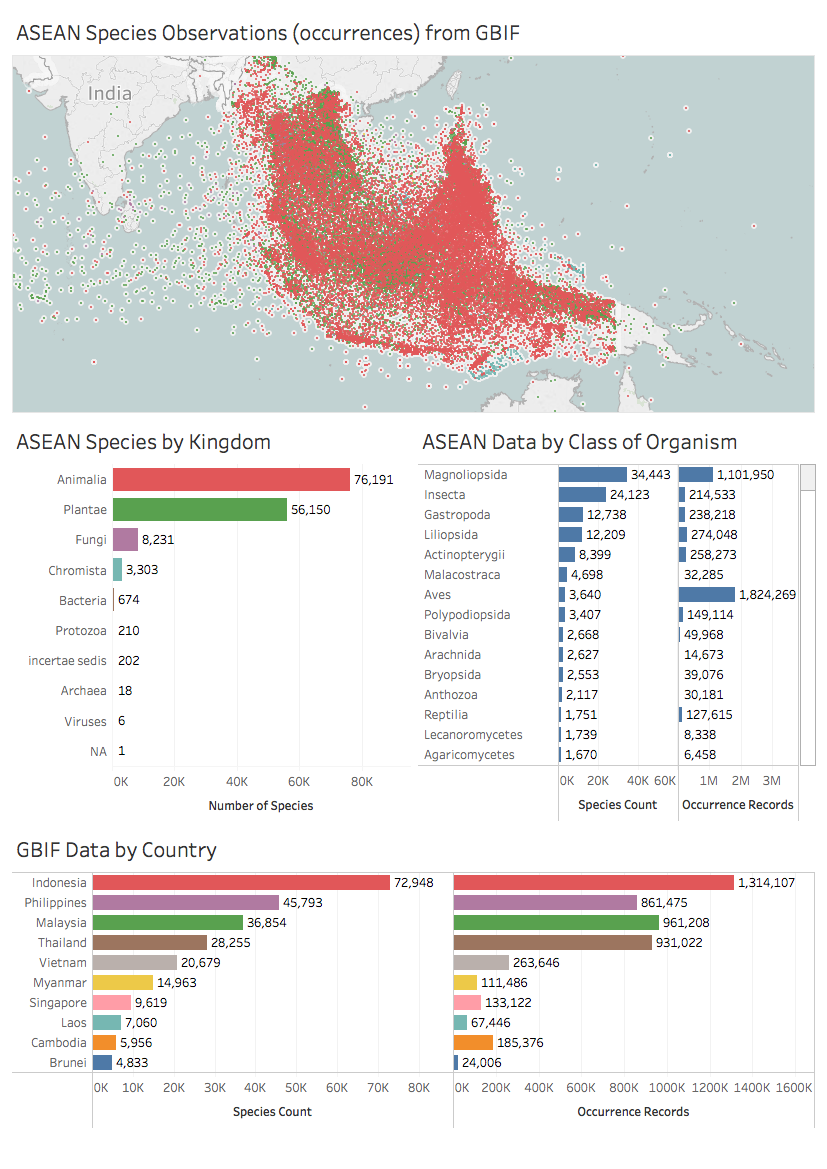
\includegraphics[width=1\linewidth]{images/asean_biodiversity} 

}

\caption{Species Occurrence Records in ASEAN Countries}\label{fig:biodiv}
\end{figure}

Figure \ref{fig:biodiv} reveals that the available species data for
ASEAN countries is dominated by information on animal (Animalia) species
followed by plants (Plantae) and fungi. GBIF does not consistently
include data on viruses and this will therefore be under-represented in
this data. Turning to the class of organisms, the data is dominated by a
class of plant species (Magnoliopsida) which also account for a large
number of observation records, followed by insects (Insecta), snails
(Gastropoda), Liliopsida (a class containing the Lily Family) and
Malacostraca such as crabs, lobsters, and shrimps. In reviewing this
data note that a common feature across GBIF data is that observational
data (occurrences) are dominated by birds (Aves) because humans display
a marked tendency to record and submit bird observations

Figure \ref{fig:biodiv} also reveals that the availability of data on
biodiversity within the ASEAN region varies considerably between
countries with Indonesia coming top in terms of both the number of
recorded species and observations in GBIF with Brunei recording the
smallest numbers. This will reflect the size of countries and also the
extent to which the scientific community and taxonomic collections have
made their basic taxonomic data available to GBIF.

Recent years have witnessed dramatic improvements in the availability of
species information in digital form. However, it is important to bear in
mind that this data will almost always represent a limited set of the
overall data and of actual biodiversity within a country or region. This
is particularly true for marine species with the marine environment
representing one of the least explored and documented environments on
earth.

\hypertarget{marine-species-in-the-biodiversity-data}{%
\subsection{Marine Species in the Biodiversity
Data}\label{marine-species-in-the-biodiversity-data}}

Marine species are a subset of the biodiversity data for the region.
However, it is important to recognise that the description of a species
as marine is not straightforward in practice because they may exist in
multiple habitats. Specifically, using the classification adopted by the
World Register of Marine Species (see below) a species may occupy one or
more of the following environments:

\begin{itemize}
\tightlist
\item
  terrestrial
\item
  freshwater (aquatic)
\item
  brackish (freshwater/saltwater boundary)
\item
  marine
\end{itemize}

A species may therefore be found in multiple environments, or it may
occupy a particular habitat at one stage of its life cycle and another
habitat at a later stage. This makes the strict isolation of marine
species difficult. As we will see below the common plant pathogen
\emph{Fusarium oxysporum} is widespread in soils but is also a marine
organism according to the World Register of Marine Species
(\href{http://www.marinespecies.org/aphia.php?p=taxdetails\&id=100523}{WoRMS}).
This presents the difficult challenge of distinguishing between
terrestrial fungi and marine fungi. A second example is provided by
mosquitoes (genus Anopheles) that have been a major focus of attention
in the scientific and the patent literature. These insects are aquatic
in the early stage of their life cycle and lay eggs in water during the
adult stage. Similarly, in the case of animal organisms some fish may
breed in freshwater but spend the majority of their life cycle in a salt
water marine environment. In the case of plants these may be found in
salt marshes, lagoons, beaches and other coastal environments and extend
into underwater habitats.

As this makes clear, drawing a distinction between marine and non-marine
organisms can be a challenge and requires close attention to detail. In
this report following exploration of the species data we adopt the
approach of excluding terrestrial species wherever possible. Based on
investigation of some plant species and fungi we limit plant species to
those with a coastal distribution (such as mangroves) and generally
exclude fungi except where they are demonstrably of marine origin.

To identify Marine species in the GBIF data we used a reference list of
marine species binomial names from the World Register of Marine Species
that we reduced to 398,000 binomial names for text mining purposes. We
identified 28,000 marine species names in GBIF data that appear in the
reference list from WoRMS. We then retrieved the available environmental
data about those species using the Lifewatch Belgium web service. GBIF
data on marine species appearing in WoRMS is summarised in Figure
\ref{fig:marine}.

\begin{figure}

{\centering 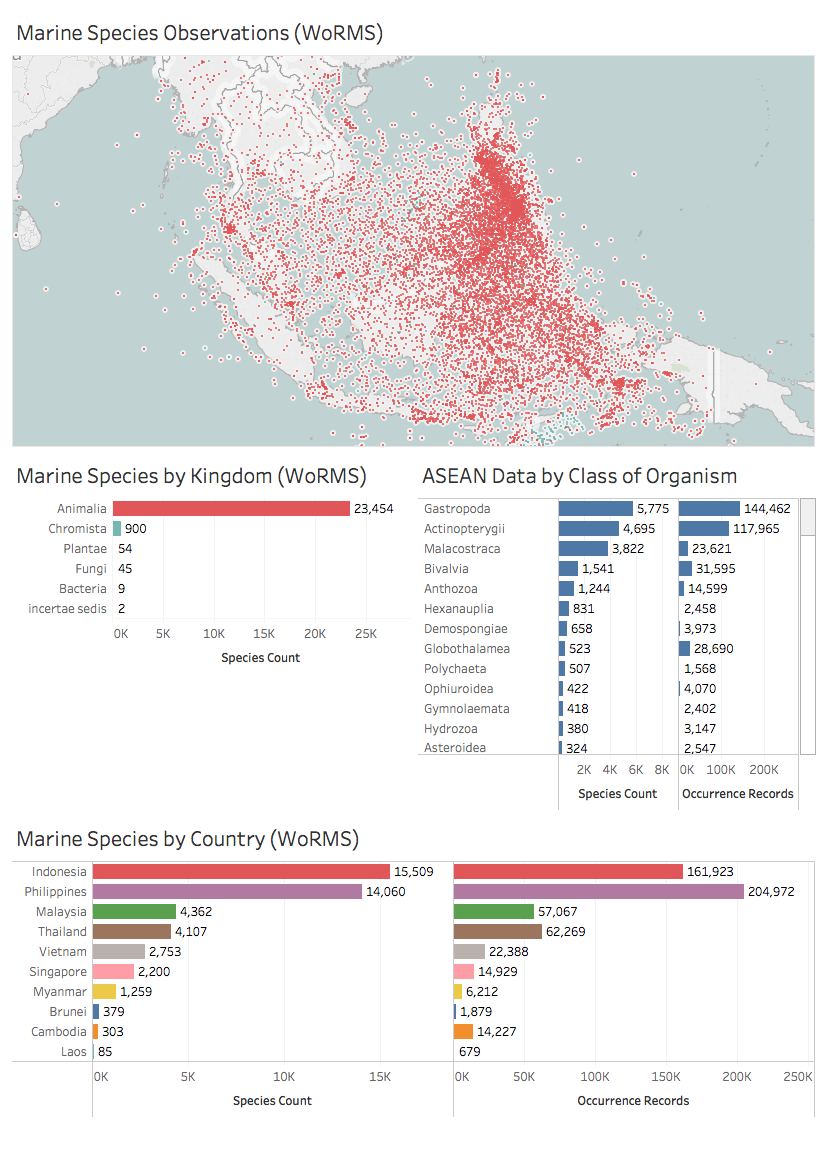
\includegraphics[width=1\linewidth]{images/asean_marine_biodiversity} 

}

\caption{Occurrence Records for Marine Species in ASEAN Countries}\label{fig:marine}
\end{figure}

Figure \ref{fig:marine} reveals, as we might expect, that the number of
species is dominated by Animalia, notably gastropods, followed by
Actinopterygii, ray-finned bony fish, Malacostraca (crabs, shrimp,
lobster), molluscs (Bivalvia), Anthozoa (marine invertebrates including
corals and gorgonians) and Hexanauplia or crustaceans such as copepods.
Interestingly, while the rankings for country level data only undergo
minor change with Singapore moving up one ranking, the Philippines moves
to the top ranking in terms of the number of recorded occurrences for
marine species. However, as we will see in the next section, in recent
years marine research in the Philippines has displayed a declining
trend.

\hypertarget{conclusion}{%
\subsection{Conclusion}\label{conclusion}}

In this section we have provided a brief overview of the available data
on biodiversity and marine biodiversity in the ASEAN region. As we have
emphasised our ability to interrogate the scientific and patent
landscapes for marine biodiversity in the ASEAN region is fundamentally
constrained by access to data about biodiversity in the region. In many
countries this is improving as countries recognise the value of
digitising their biodiversity data and make it available through the
Global Biodiversity Information Facility (GBIF).

As we will see in the following sections, the availability of taxonomic
information or biodiversity informatics is also important for our
ability to map and understand research and research and development
involving marine species within and beyond the ASEAN region.

\hypertarget{references}{%
\subsection{References}\label{references}}

GBIF occurrence datasets as used in this report are publicly available
for download as follows and should be cited using the supplied DOIs.

\begin{enumerate}
\def\labelenumi{\arabic{enumi}.}
\tightlist
\item
  \href{https://www.gbif.org/occurrence/download/0020859-180131172636756}{Brunei
  darussalam, DOI 10.15468/dl.ny8aam}
\item
  \href{https://www.gbif.org/occurrence/download/0020860-180131172636756}{Cambodia,
  DOI: 10.15468/dl.22e1ct}
\item
  \href{https://www.gbif.org/occurrence/download/0020862-180131172636756}{Indonesia,
  DOI: 10.15468/dl.cwwjsn}
\item
  \href{https://www.gbif.org/occurrence/download/0020864-180131172636756}{Lao
  people's democratic republic, DOI: 10.15468/dl.x7kr9j}
\item
  \href{https://www.gbif.org/occurrence/download/0020868-180131172636756}{Malaysia,
  DOI: 10.15468/dl.3b9yw3}
\item
  \href{https://www.gbif.org/occurrence/download/0020878-180131172636756}{Myanmar,
  DOI: 10.15468/dl.2czwzg}
\item
  \href{https://www.gbif.org/occurrence/download/0020868-180131172636756}{Philippines,
  DOI: 10.15468/dl.fi2kit}
\item
  \href{https://www.gbif.org/occurrence/download/0020880-180131172636756}{Singapore,
  DOI: 10.15468/dl.ribxsw}
\item
  \href{https://www.gbif.org/occurrence/download/0020885-180131172636756}{Thailand,
  DOI: 10.15468/dl.vzhaey}
\item
  \href{https://www.gbif.org/occurrence/download/0020888-180131172636756}{Viet
  Nam, DOI: 10.15468/dl.8qivwd}
\item
  \href{https://www.gbif.org/occurrence/download/0000637-171219132708484}{South
  East Asia and Pacific bounding box, DOI: 10.15468/dl.e7bm2i}. Polygon:
  ((89.296875 -11.591978551846823, 89.296875 30.388035892267144,
  161.71874999999997 30.388035892267144, 161.71874999999997
  -11.591978551846823, 89.296875 -11.591978551846823))
\end{enumerate}

\hypertarget{scientific}{%
\chapter{The Scientific Landscape for Marine Genetic Resources in the
ASEAN Region}\label{scientific}}

In this section we examine the scientific landscape for research
involving marine species. In total we identified 6,659 scientific
publications in Clarivate Analytics Web of Science Core Collection that
contained a marine species listed in the World Register of Marine
Species (WoRMS) database. ASEAN researchers were co-authors on 77\%
(5,109) of the publications. The 6,659 records contained 3,685 marine
species after the exclusion of common model organisms.

Figure \ref{fig:marineres} displays a snapshot overview of activity for
marine species in the region. \footnote{This data can be explored
  interactively in an online \href{link}{Tableau Public workbook}}

\begin{figure}

{\centering 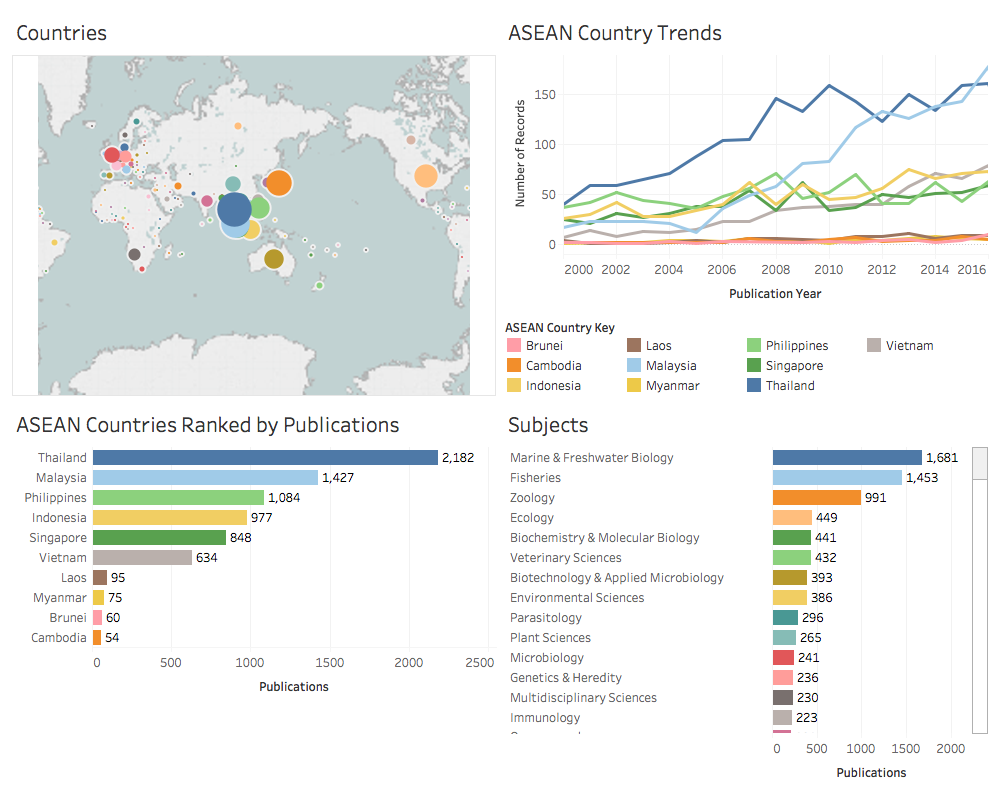
\includegraphics[width=1\linewidth]{images/aseanmarinlit_overview} 

}

\caption{Overview of Research Activity for Marine Species in ASEAN countries}\label{fig:marineres}
\end{figure}

In Figure \ref{fig:marineres} we can immediately see that marine
research in the ASEAN region encompasses countries within and outside
the region. This reflects the increasingly international nature of
modern scientific research and marine research. We can also observe
significant variation in levels of marine publications between ASEAN
countries with respect to trends that reflect the underlying emphasis
and strength of each country with respect to marine research. Finally,
information on the subject area of research reveals the prominence of
Marine \& Freshwater Biology (as we would expect) along with more
applied fields such as Biotechnology \& Applied Microbiology and
Parasitology or Immunology that provide an indication of potentially
more commercially oriented research areas.\footnote{Subject Areas refer
  to Web of Science Subject Categories which seek to describe the
  subject area of journals where articles are published. A single
  journal may fall into more than one category and are used here as a
  proxy for summarising research subjects}

\hypertarget{trends-by-country}{%
\subsection{Trends by Country}\label{trends-by-country}}

The presentation of trends by country in Figure \ref{fig:marineres} has
the effect of pressing countries with lower level marine research
outputs to the bottom of the graph. We gain a clearer view of country
level trends in Figure \ref{fig:marinetrends} where the data for each
country is presented in separate panels. In Figure
\ref{fig:marinetrends} we present the data as a scatterplot and then add
a smoothed trend line (using Loess or locally weighted smoothing)
between the data points.

\begin{figure}

{\centering 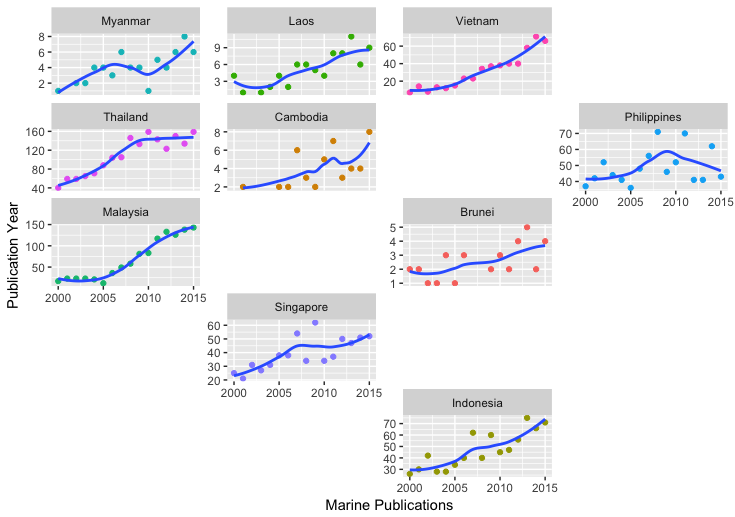
\includegraphics[width=1\linewidth]{images/country_trends} 

}

\caption{Country Trends for Research on Marine Genetic Resources in the South East Asia Region}\label{fig:marinetrends}
\end{figure}

This reveals, that in general all countries within the region have
displayed an increase in publications on marine research over time with
Myanmar, Laos, Cambodia and Brunei exhibiting less than 10 publications
per year across all years. For countries with higher levels of activity,
Thailand emerges as the leading country for research involving marine
species. However, research outputs plateaued from 2010 onwards before
staging a more recent increase in 2016. In the meantime, as can more
clearly be seen in Figure \ref{fig:marinetrends}, Malaysia has displayed
a steeply rising trend in research outputs that has overtaken Thailand.
In contrast with countries throughout the region that display a rising
trend, the Philippines displays a declining trend from approximately
2008 onwards that may reflect either a change in the orientation or
research outputs (for example with a more applied focus that place less
emphasis on publications) or a decline in research investment in marine
research.

Research outputs, in the form of peer reviewed research articles and
scientific publications, reflect underlying investments and incentives
for scientific research in the marine and terrestrial aquatic
environments. As we have seen, while varying in intensity, in the
majority of ASEAN countries marine organisms are an increasing or
emerging focus of scientific publications. We now take a closer look at
the nature of research activity.

\hypertarget{marine-species-research}{%
\subsection{Marine Species Research}\label{marine-species-research}}

Figure \ref{fig:taxonomysubjectarea} presents an overview of marine
research in the ASEAN region from the perspective of the species that
are a focus of research.\footnote{This dashboard can be explored
  interactively \href{link}{Tableau Public workbook}} For the top ten
species we provide a set of short fact sheets in Chapter \ref{species}
of the report. Here we present a short summary for the top species.

\begin{figure}

{\centering 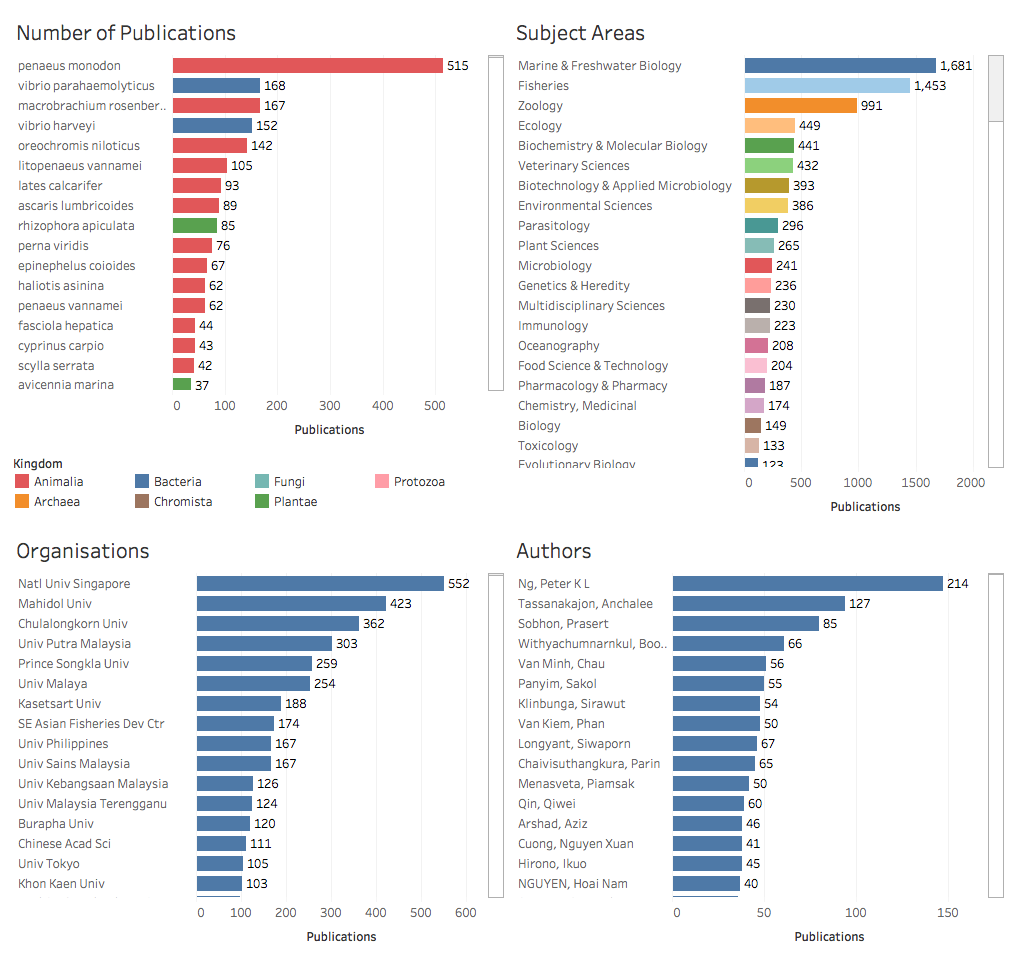
\includegraphics[width=1\linewidth]{images/aseanmarinlit_species_overview} 

}

\caption{Top Marine Species Overview}\label{fig:taxonomysubjectarea}
\end{figure}

In considering Figure \ref{fig:taxonomysubjectarea} a number of the top
species are shrimps associated with the rapid growth of aquaculture in
the region from the late 1990s onwards \citep{Hishamunda_2009}.

Figure \ref{fig:taxonomysubjectarea} reveals that the species that the
Giant Tiger Shrimp (\emph{Peneaus Mondon}) is a major focus of research
activity that reflects the economic importance of the species in the
aquaculture sector within the ASEAN region. Research with respect to
\emph{Peneaus Mondon} is directed towards maximizing yields. A
significant proportion of the literature focuses on understanding
\emph{P. mondon} immune responses to viral and bacterial pathogens that
are responsible for large scale mortality in tiger shrimps, notably
White Spot Syndrome Virus, Yellow Head Virus and \emph{Vibrio harveyi}
\citep{Wongteerasupaya_1995, Ponprateep_2011, Jaree_2012}.

The second ranking animal species in the data also relates to
aquaculture. \emph{Macrobachium rosenbergii} (the Giant River Prawn and
the Giant Freshwater Prawn) is widely fished and is the main freshwater
shrimp cultivated within the commercial aquaculture industry
\citep{Macrobrachium_2012}.\footnote{IUCN Red List at
  \url{http://www.iucnredlist.org/details/197873/0}} While this is a
freshwater species, females move into brackish estuarine waters to lay
their eggs. As with \emph{P. mondon} research is directed towards
maximizing yields and reducing mortality from pathogens such as White
Tail Disease virus \citep{Bonami_2011}. Improvements to broodstock
genetics \citep{Karaket_2012, Nguyen_Thanh_2015, Thanh_2010} as well as
improvements to prawn feed \citep{Kangpanich_2016} have been a
significant focus of research activity.

\emph{Oreochromis niloticus} is a species of Tilapia, a cichlid fish
native to the Nile basin in Africa and coastal rivers of
Israel.\footnote{Encyclopaedia of Life at
  \url{http://eol.org/pages/356343/data?toc_id=4\#1448}} It is an
economically important species introduced into the ASEAN region and
elsewhere because it is fast growing. The literature focuses on issues
such as genetic improvement \citep{Bentsen_1998}, options for rice paddy
field polyculture in conjunction with other species \citep{Vromant_2002}
, and salt tolerant hybrids for aquaculture in coastal ponds for this
freshwater species \citep{Kamal_2005}.

\emph{Litopenaeus vannamei} is the world's dominant cultivated shrimp.
It grows as a juvenile in estuarine environments and lives in marine
salt water as an adult. South East Asia has witnessed dramatic growth in
aquaculture for this species, notably in Thailand and China. Improving
breeding stocks \citep{Nimrat_2006}, protection against infectious
myonecrosis \citep{Silva_2010}, and alternatives to the use of
antibiotics such as the use of probiotics \citep{Nimrat_2011} feature
prominently in the literature for this major species.

\emph{Lates calcarifer} is the Barramundi or Asian seabass and is a
widely distributed demersal fish ranging from the Persian Gulf through
South East Asia and Papua New Guinea.\footnote{Demersal fish are bottom
  feeders in what is known as the demersal zone} It is typically found
in estuaries, coastal waters, lagoons and rivers. Research has focused
on aquaculture for this species including understanding the natural
history of the species \citep{Shadrin_2015} and fish feed
\citep{Shansudin_1997, Mohd_Yusof_2010} including the use of local
seaweed species \citep{Shapawi_2015}.

\emph{Ascaris lumbricoides} is the large roundworm and is responsible
for causing ascariasis in humans. While \emph{A. lumbricoides} is
aquatic and recorded by WoRMS as a marine species it is excluded from
further analysis because the focus of the scientific literature in the
ASEAN region is on soil transmitted helminth infections in humans,
including in coastal areas, rather than the marine environment as such
\citep{Montresor_2007}.

\emph{Perna viridis} is commonly known as the Indian Green Mussel.
Research in relation to this species in ASEAN countries focuses on
issues such as the impacts of metal concentrations, notably heavy metals
on speciation, the implications of contamination for human health and
the potential use of the species for wider biomonitoring of heavy metal
contamination \citep{Yap_2002, Yap_2004, Yap_2003}. Other research
addresses concentrations of shellfish toxins and \emph{Vibrio
parahaemolyticus} in \emph{P. viridis} \citep{Marasigan_2001} along with
issues such as suspension feeding behaviour
\citep{Hawkins_1998, Tan_2016} and genetic diversity \citep{Ye_2015}. As
this suggests, land based run offs of contaminants into the marine
environment in the ASEAN region has become a significant focus of
research for this economically important species.

\emph{Epinephelus coioides} is the Orange Spotted Grouper or Estuary
Cod. This is an IUCN Red List near threatened species that in its
juvenile stage is found in estuaries and mangroves and as adults in
brackish water and coastal reefs. \footnote{\url{http://www.fishbase.org/summary/6465}}
It is a commercially important species including in aquaculture.
Research in the ASEAN region has included work on cell lines
\citep{Qin_2006}, feeding performance \citep{Doi_1997, Eusebio_2004} and
the immune system of this important commercial species
\citep{Zhou_2011, Guo_2012}.

Two bacteria feature prominently in marine research in the ASEAN region.
The first of these is \emph{Vibrio parahaemolyticus}, a gram negative
bacteria that is found in estuarine, coastal and marine waters.
\emph{Vibrio parahaemolyticus} is now a globally distributed species
associated with vibriosis through the consumption of raw shellfish or
exposure to contaminated water \citep{Nair_2007}. Within the literature
for ASEAN countries the main focus is on the impact of contamination in
aquaculture, including detecting strains associated with
infection\citep{RAHMAN_2006} and vaccines \citep{Hu_2011}. The risks of
mortality in shellfish stocks and consequent mortality rates are
combined with increasing awareness of the problem of antibiotic
resistance and the quest for alternatives such as botanical extracts
sourced from ASEAN countries
\citep{Sivasothy_2013, Nguyen_2016, Tinh_2016}.

The second major bacterial species is \emph{Vibrio harveyi}, a
Gram-negative, bioluminescent and common marine bacterium in the same
genus as \emph{V. parahaemolyticus}. It is common in the gut of many
tropical marine organisms with a small number of strains being
pathogenic. While the bacteria is normally benign, pathogenic
sub-strains are particularly associated with impacts on shrimps such as
\emph{P. mondon}, with the ASEAN literature focusing on detection and
the use of natural compounds, including from marine cyanobacteria
\citep{Ponprateep_2009, Maneechote_2016, Maneechote_2016}

\emph{Rhizophora apiculata} is a widespread intertidal mangrove species
in the ASEAN region. The species is used for firewood and is also a
focus of commercial mangrove silviculture in the region
\citep{Rhizophora_2015}. A second important mangrove species is
\emph{Avicennia marina}, known as the grey or white mangrove that is
widely distributed throughout the ASEAN region and beyond. It takes form
as a shrub or tree and has a range of uses as a food source, in
construction and medicine \citep{Avicennia_2008}. Research on this
species in the ASEAN region has focused on issues such as genetic
structure and variation \citep{ARNAUD_HAOND_2006, Giang_2003}, the
impacts of aquaculture water on mangroves \citep{Vaiphasa_2007},
biodiversity \citep{Zhila_2013}, mangrove restoration \citep{Aung_2011}
and new plant extract for alopecia treatment
\citep{Jain_2015, Jain_2014}.

As this brief summary of the major species suggests, the marine data is
dominated by species that are commercially important in aquaculture
within the region. This comes into clearer focus if we examine the
relationship between research on species grouped on the genus level and
the subject areas of publications.

Figure \ref{fig:sankeygenussubject} presents a Sankey diagram of the
flow between research on the species and Subject Areas presented in
\ref{fig:taxonomysubjectarea}. A Sankey diagram is typically used to
display the flow of energy, in this case investments in research on
species grouped on the genus level, and the intended audiences
represented by the subject areas.

We can clearly see in Figure \ref{fig:sankeygenussubject} that research
on Penaeus (e.g.~Tiger Prawn) genus primarily flows into fisheries
followed by Marine and Freshwater Biology. The link between research on
Penaeus and Vibrio is represented by Immunology and Veterinary Science.
In contrast work on mangroves (represented by Avicennia and Rhizophora)
is more concentrated in Environmental Sciences (for Avicennia) and
additionally Marine and Freshwater Biology, Ecology and Plant Sciences
for Rhizophora. This suggests a more basic research orientation for our
mangrove species as discussed above.

\begin{figure}

{\centering 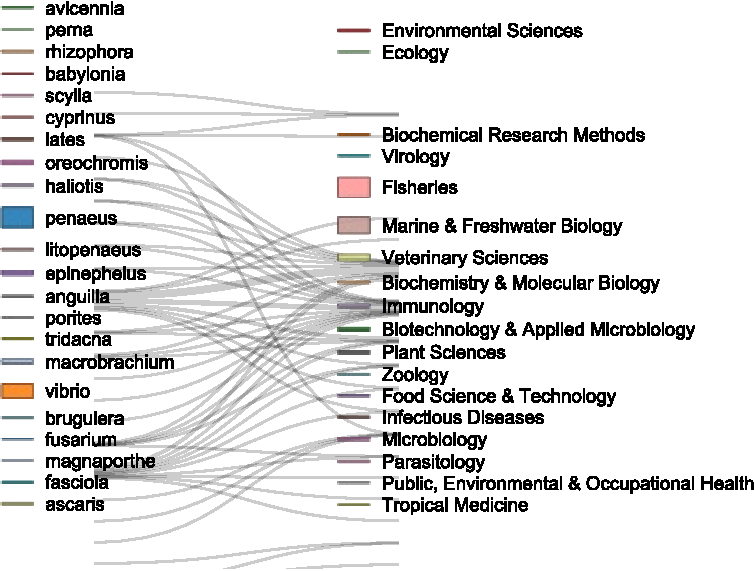
\includegraphics[width=1\linewidth]{asean_marine_files/figure-latex/sankeygenussubject-1} 

}

\caption{Flows of Publications on Species into Subject Areas}\label{fig:sankeygenussubject}
\end{figure}

Figure \ref{fig:sankeygenussubject} provides the first indication that
marine research may be directed in multiple directions, from basic
taxonomic and ecological research, to commercially oriented research
that focuses on enhancing productivity and addressing problems such as
pathogens for commercially valuable species.

In practice, research on species takes place in networks that can be
explored on multiple levels.

First, researchers are typically performing research on more than one
species. For example, work on pathogens of \emph{P. mondon} and other
shellfish will include reference both to the source species (\emph{P.
mondon}) and the target species.

Second, there has been a growing trend towards the internationalisation
of research collaborations represented by collaborations between
researchers outside their home countries and regions. This is typically
supported by national research institutions, such as research councils,
and home institutions administering funds on behalf of national
organisations. These investments form a network of collaboration between
countries that are underpinned by financial investments in research,
typically by national research councils or their equivalent.

Third, collaboration networks between researchers involve
inter-institutional relationships including flows of research funding,
equipment, students and post-doctoral researchers.

Finally, there are the networks of relationships between researchers who
build the wider inter-institutional network and communities of
researchers working on particular marine species and particular
problems.

To gain a fuller understanding of the characteristics of research on
marine genetic resources in the ASEAN region we will explore each of
these networks in turn.

\hypertarget{the-species-network}{%
\subsection{The Species Network}\label{the-species-network}}

Figure \ref{fig:speciesnetwork} displays the network relationships
between publications involving marine species where there are more than
10 publications referencing the species. The dots represent nodes in the
network and are sized based on the number of records. The lines or edges
are based on the number of publications where the species appear in the
same publication with thickness representing the number of shared links.
The colours in this case refer to the kingdom for each organism as in
Figure \ref{fig:taxonomysubjectarea}.

\begin{figure}

{\centering 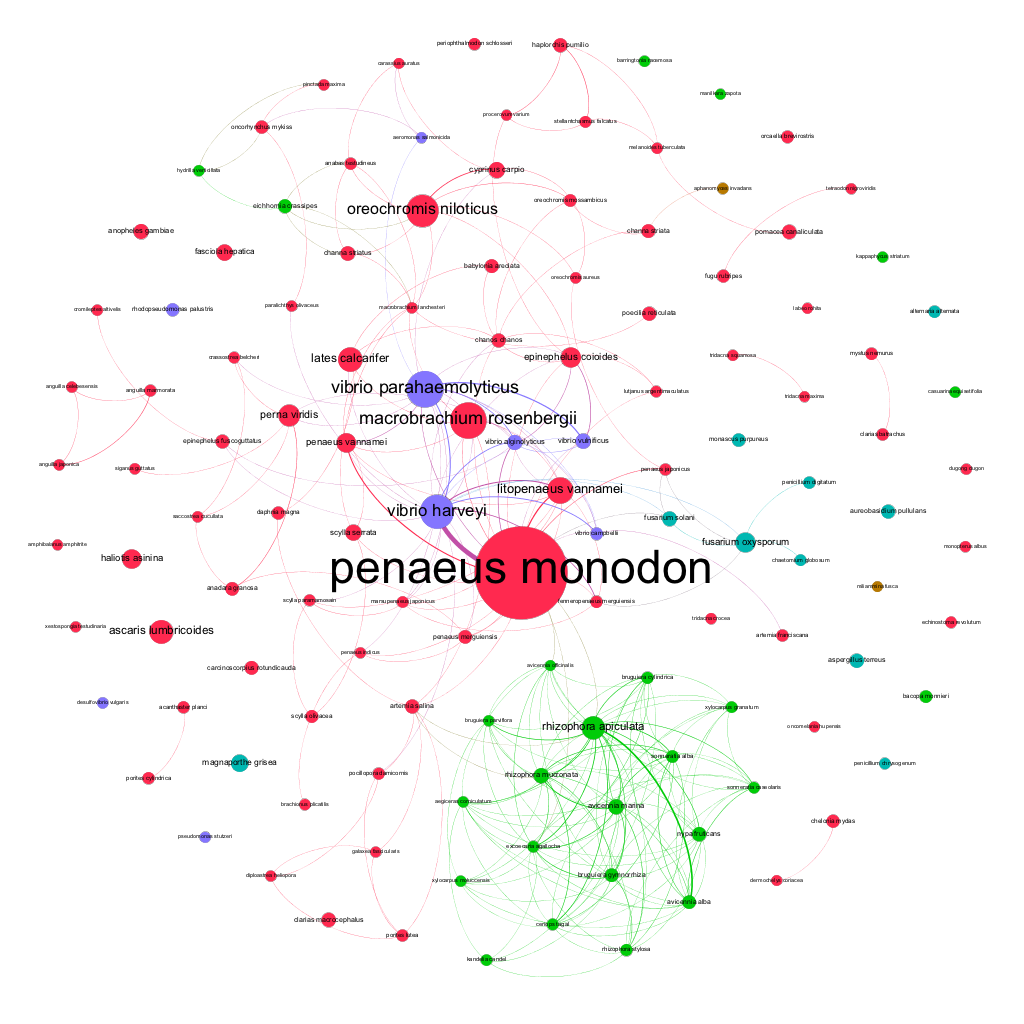
\includegraphics[width=1\linewidth]{images/aseanmarinlit_species_network_plus10} 

}

\caption{Network of Species that are the Focus of Research}\label{fig:speciesnetwork}
\end{figure}

What is powerful about this form of visualisation is that we can
immediately see that a strong relationship between the Vibrio pathogenic
viruses and important aquaculture species, notably prawns and shrimps
such as \emph{Penaeus mondon}, \emph{Macrobrachium rosenbergii} and
\emph{Litopenaeus vannamei} among others such as \emph{Penaeus
vannamei}. We can also see that research on plants, dominated by
mangroves (in green) forms a distinctive cluster of research but also
links through \emph{Avicennia marina} and \emph{Rhizophora apiculata} to
research on \emph{Peneaus mondon} and related species \citep{Hai_2005}.

We can apply this same approach to a broader overview of the scientific
landscape for marine research at the level of the analysis of
international and regional level research collaborations to which we now
turn.

\hypertarget{country-networks}{%
\subsection{Country Networks}\label{country-networks}}

In total 136 countries appeared in the ASEAN data for research involving
marine genetic resources (see Figure \ref{fig:marineres} above).
Collaborations between countries involved in marine research can be
visualized as a network. Figure \ref{fig:marineres} below displays the
country collaboration network where there are two or more publications
involving researchers from those countries. Once again the size of the
nodes reflects the number of publications.

\begin{figure}

{\centering 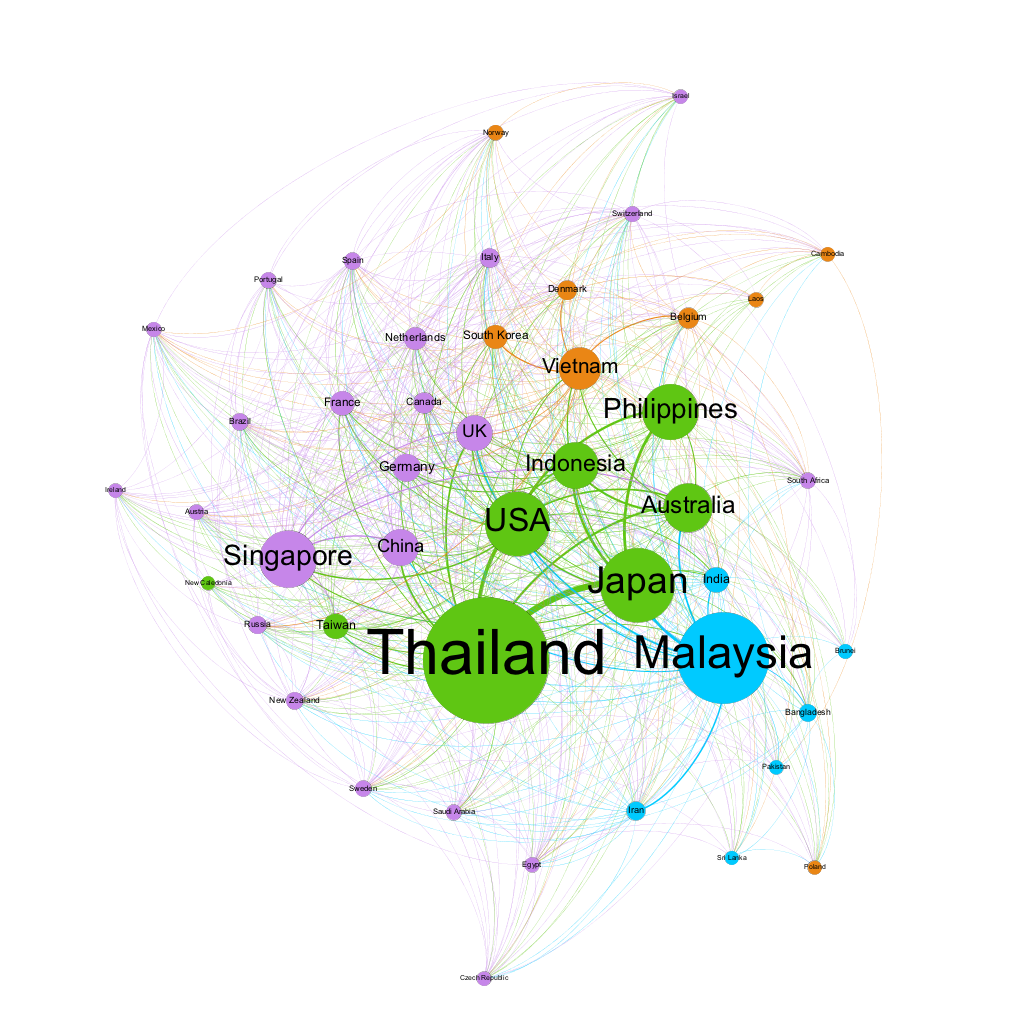
\includegraphics[width=1\linewidth]{images/aseanmarinlit_country_network} 

}

\caption{Country Collaboration Networks for Marine Genetic Research in the ASEAN region}\label{fig:countrynetwork}
\end{figure}

In Figure \ref{fig:countrynetwork} the country nodes are sized based on
the number of records that involve a publication with an author from the
country. The lines (edges) represent publications by authors from both
countries with the weight of the lines indicating the number of
publications. The colours denote communities of collaborating countries
based on the calculation of the strength of the links between them
compared with the strength of connections between all other nodes
(countries) \citep{Blondel_2008}. This allows us to see the distinctive
network connections between ASEAN countries and other countries.

Figure \ref{fig:countrynetwork} reveals 4 main country network clusters.
The largest network cluster is represented by Thailand with strong
connections with Japan, the United States, Australia, the UK and China
along with the Philippines. Malaysia displays weaker links with a number
of these countries but is distinctive for its links with India,
neighbouring Brunei, Bangladesh, Pakistan and Sri Lanka. Singapore
displays a weaker but wider set of connections with other countries,
while Vietnam forms part of a network with South Korea, Denmark, Norway,
Laos and Cambodia. The importance of mapping these collaboration
networks is that they reflect underlying financial investments in the
form of research funding, investments in student training, equipment and
materials.

\hypertarget{the-funding-network}{%
\subsection{The Funding Network}\label{the-funding-network}}

This network of relationships between countries reflects underlying
national investments in the driving force behind all research: research
funding. Data on research funding is difficult to access and has only
been available in \emph{Web of Science} from 2008 onwards and suffers
from a lack of uniformity in the data requiring extensive cleaning.
However, we can gain a partial insight into the major funding agencies
involved in marine genetic resources in the ASEAN region in the network
map in Figure \ref{fig:fundingnetwork}. This network displays funding
organisations that appear in the acknowledgements of more than 20
publications in the ASEAN Web of Science dataset.

\begin{figure}

{\centering 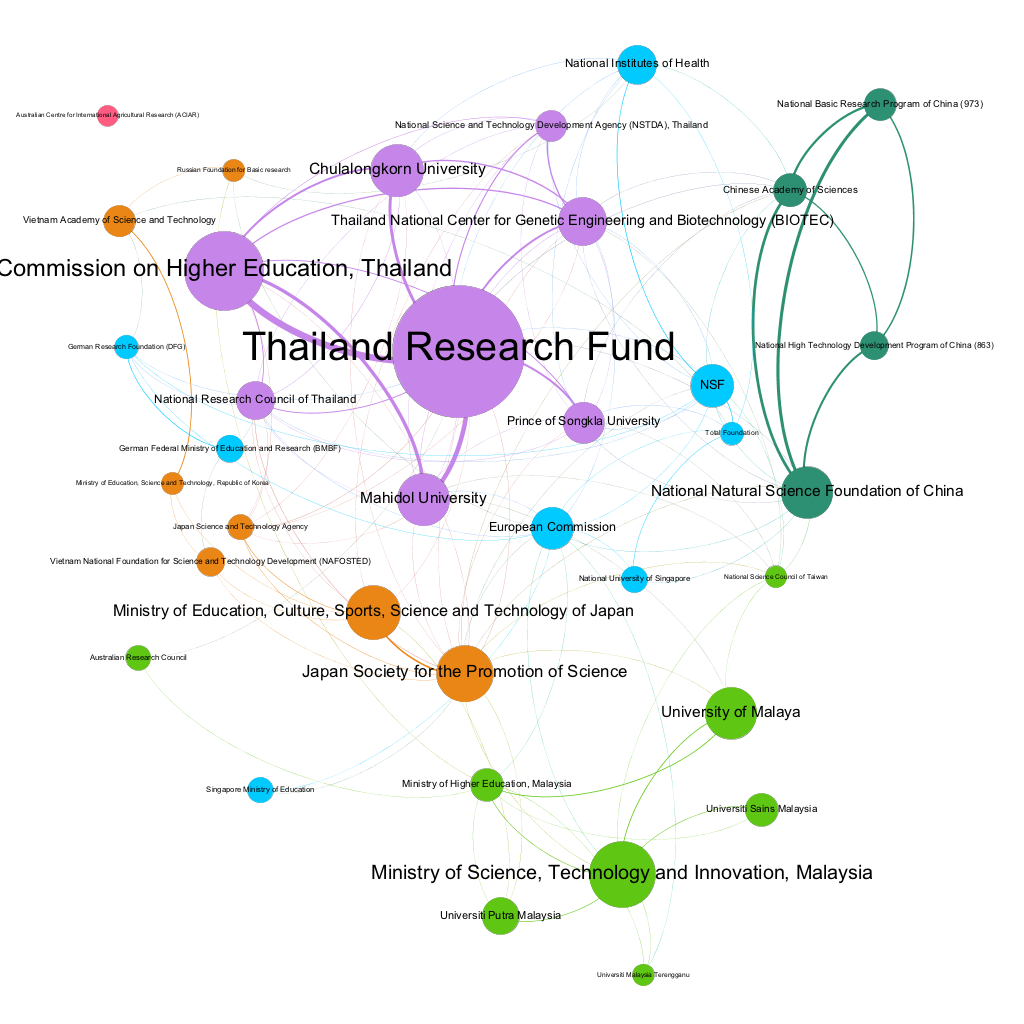
\includegraphics[width=1\linewidth]{images/aseanmarinlit_fundingnetwork} 

}

\caption{Major Funding Networks for Marine Genetic Research in the ASEAN region}\label{fig:fundingnetwork}
\end{figure}

In considering Figure \ref{fig:fundingnetwork} we immediately observe
the dominant position of the Thailand Research Fund and the Commission
on Higher Education in Thailand (officially the Office of the Higher
Education Commission or OHEC) along with universities in funding marine
research in Thailand. While this network displays rankings based on the
number of publications, rather than the size of investments, it suggests
that the strong trend in publications in marine research in Thailand
reflects dedicated funding investment. Looking outside Thailand, a
network of external funding bodies emerges in connection with
publications from Thailand in the form of the United States National
Science Foundation (through the Thailand National Research Fund and the
BIOTEC centre) as well as joint publications with research funding from
Germany. Funding Agencies from Japan appear particularly prominently in
the funding network notably through the Ministry of Education, Culture,
Sports, Science and Technology (MEXT) and the Japan Society for the
Promotion of Science. Funding organisations from China are also emerging
as a major funding source on marine research publications.

As noted above, our ability to view funding networks is presently
partial. However, we can also gain an insight into the subject areas
where research investments are being made. Figure
\ref{fig:sankeyfunding} aggregates the funding agencies by country and
displays the subject areas of research outputs focusing on the top
subject areas.

\begin{figure}

{\centering 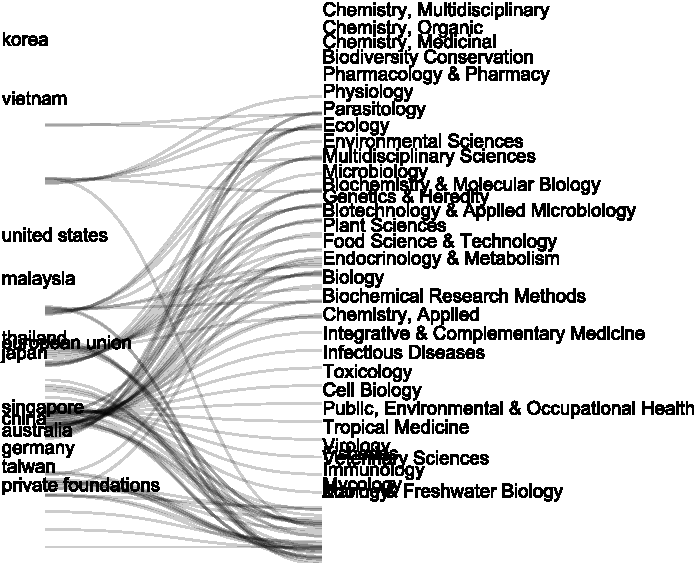
\includegraphics[width=1\linewidth]{asean_marine_files/figure-latex/sankeyfunding-1} 

}

\caption{Funding Flows through Publications on Marine Genetic Resources in the ASEAN region}\label{fig:sankeyfunding}
\end{figure}

Three points stand out in Figure \ref{fig:sankeyfunding}. The first of
these is a clear investment stream in fisheries research in the case of
Thailand that is also strong in the case of Marine \& Freshwater
Biology. The second point is the that Vietnam's research investment is
marked by an emphasis in Chemistry and Pharmacology (as are research
investments from Korea). Investment by Japan is more evenly balanced but
also includes Chemistry and Pharmacology while investments from the
European Union (through the European Commission programmes) are focused
on Fisheries, Marine \& Freshwater Biology and Zoology. While we must
emphasise that our ability to view the data is partial, and constrained
by data variability, we can nevertheless detect the main orientations of
research investments as we will see in more detail below.

\hypertarget{the-organisational-landscape}{%
\subsection{The Organisational
Landscape}\label{the-organisational-landscape}}

Collaborative research relationships between countries in marine
research reflect underlying collaborations between individual
researchers and research teams based in organisations. In total,
approximately \texttt{xxx} organisations were involved in marine
research linked to the ASEAN region. Advances in the availability of
geomapping tools, in this case the Google Maps API, made it possible to
geocode the nearly 4,000 organisations involved in marine genetic
research. Figure \ref{fig:organisationmap} displays the results along
with a selection of linked records from the National University of
Singapore. \footnote{The interactive version of this figure is
  accessible INSERT \href{}{here} and will display the results by
  institution}

\begin{figure}

{\centering 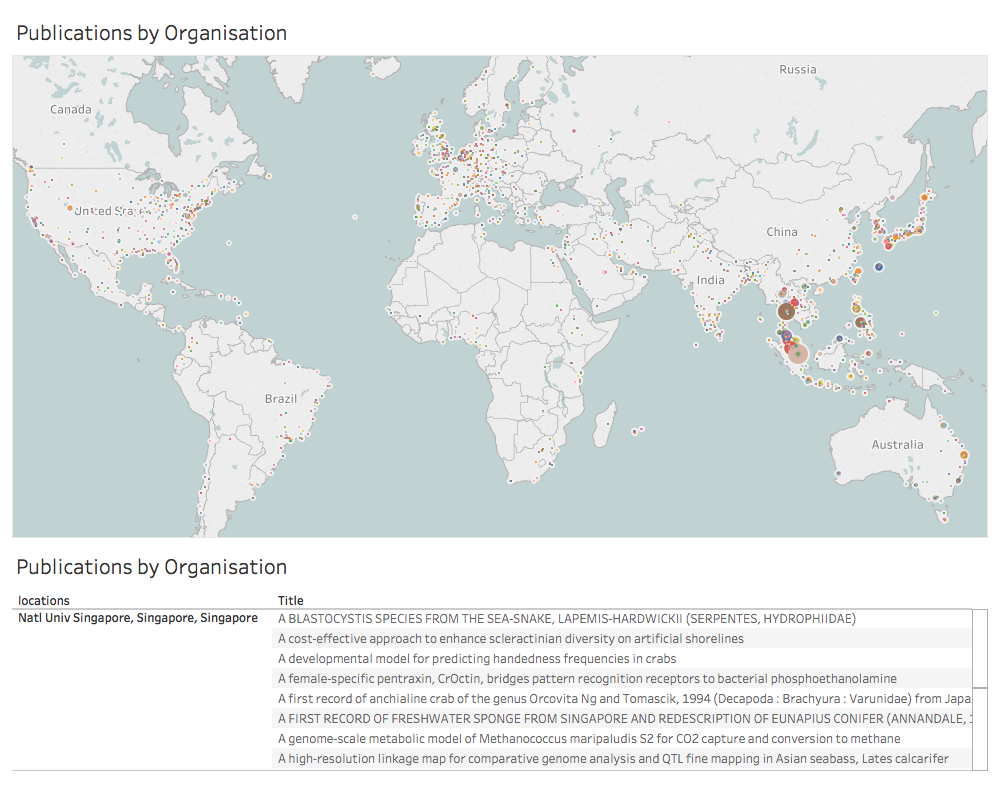
\includegraphics[width=1\linewidth]{images/aseanmarinlit_organisation} 

}

\caption{Geographic Distribution of Organisations Publishing on Marine Genetic Resources in the ASEAN Region}\label{fig:organisationmap}
\end{figure}

Figure \ref{fig:organisationmap} reveals, as we might expect, that the
major clusters of research activity is found within the ASEAN region
extending through to Japan, Australia and China. However, we can also
observe a wider set of connections including with India, Africa, Europe
and the United States that make clear the global nature of research on
the marine environment in the ASEAN region.

As with the country networks, this data can also be visualised as a
network. Figure \ref{fig:organisationnetwork} displays the network of
collaborating organisations for organisations with 20 or more
publications involving marine species. The nodes in the network are
sized on the number of publications associated with the organisation.
The lines represent the connections (in the form of co-authored
articles) between the organisations with heavier lines representing
stronger collaborative links. Finally colours seek to identify
communities based on the strength of the co-author linkages between the
actors in the network using the modularity class algorithm in Gephi for
community detection \citep{Blondel_2008}. This suggests that researchers
at the National University of Singapore lead a networked community of
researchers involving Nanyang Technology University in Singapore, the
Chinese Academy of Sciences and the University of Queensland (Australia)
among others. In contrast, Mahidol University, Chulalongkorn University
and Prince Songkla University in Thailand are all prominent in
conducting research involving marine genetic resources but have stronger
links with Tokyo University of Marine Science and Technology, Deakin
University (USA) and the University of California at Davis (USA). For
the Philippines, a strong connection emerges with the University of
Tokyo. For Vietnam, which appears on the outer edges of the network a
relationship emerges between the Vietnam Academy of Science and
Technology and the Russian Academy of Sciences with other links in the
Vietnam community to Seoul National University and Gyeongsang National
University in South Korea.

\begin{figure}

{\centering 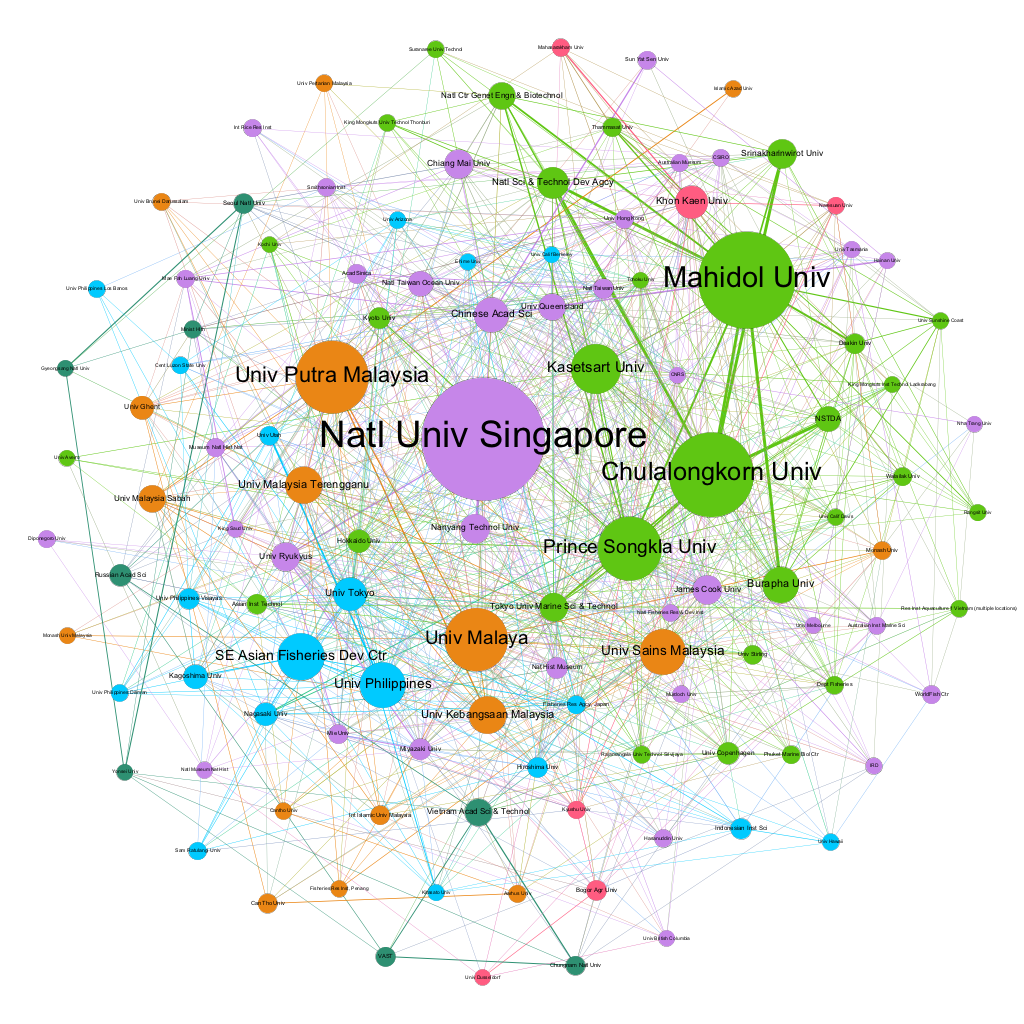
\includegraphics[width=1\linewidth]{images/aseanmarinlit_organisations_gephi} 

}

\caption{Collaboration Networks for Organisations publishing on Marine Genetic Resources in the ASEAN region based on shared publications}\label{fig:organisationnetwork}
\end{figure}

These networks are revealed through the analysis of the institutional
affiliation of authors, but they are generally hidden networks in so far
that only the parts of a network that a researcher is involved with will
be visible to them while institutional knowledge of these connections
may be limited. However, these networks are important in so far that
they represent exchanges and transfers of knowledge, the joint
generation of new knowledge and financial investments in personnel and
research in the form of research funding. One question, to which we will
return in the analysis of the patent data, is the extent to which
organisations involved in research networks on marine genetic resources
in the ASEAN region are also involved in patent activity.

We can perform a similar analysis for the researchers whose
collaborations establish these networks. Figure \ref{fig:authornetwork}
visualises the network of authors with 20 or more publications involving
marine organisms and uses a community detection algorithm to identify
clusters of collaborating authors. We will return to this analysis in
more detail in consideration of the patent data. However, for the moment
we observe the prominence of Anchalee Tassanakajon at Chulalongkorn
University in Thailand who has conducted extensive research on the tiger
shrimp (\emph{Penaeaus mondon}) and on the outer edge of the network
Nobel Prize winner Sydney Brenner who has collaborated with Byrappa
Venkatesh from the Institute for Molecular \& Cell Biology in Singapore
in ground breaking research on the puffer fish genome (\emph{Fugu
rubripes}) \citep{Brenner_1993}.

\begin{figure}

{\centering 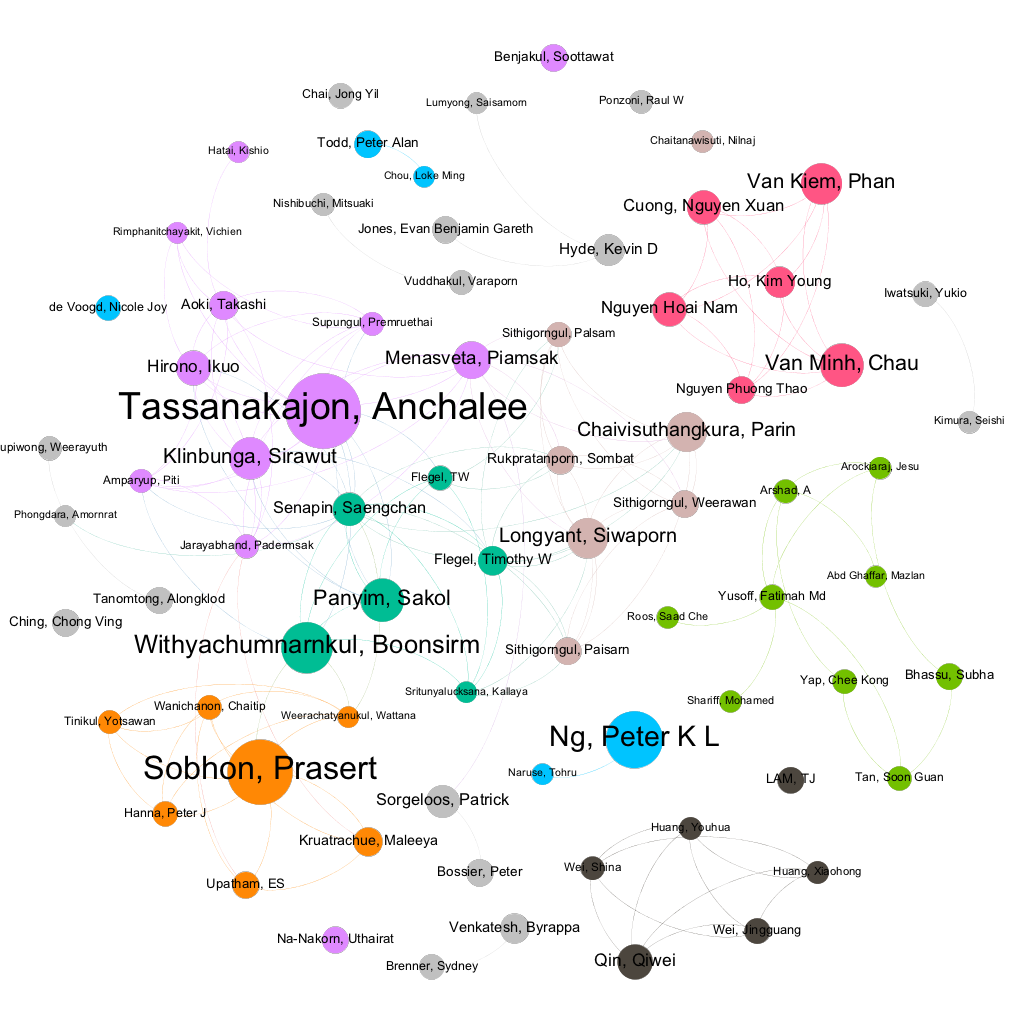
\includegraphics[width=1\linewidth]{images/aseanmarinlit_author20plus} 

}

\caption{Collaboration Networks for Researchers publishing on Marine Genetic Resources in the ASEAN region based on shared publications}\label{fig:authornetwork}
\end{figure}

We can gain a clearer picture of the relationship between the leading
researchers in these clusters and the species involved in their research
by placing the researchers and the species that are the target of their
research in the same network graph. Figure
\ref{fig:speciesresearchernetwork} displays the top species, based on
the number of records in green and the main researchers in pink.

\begin{figure}

{\centering 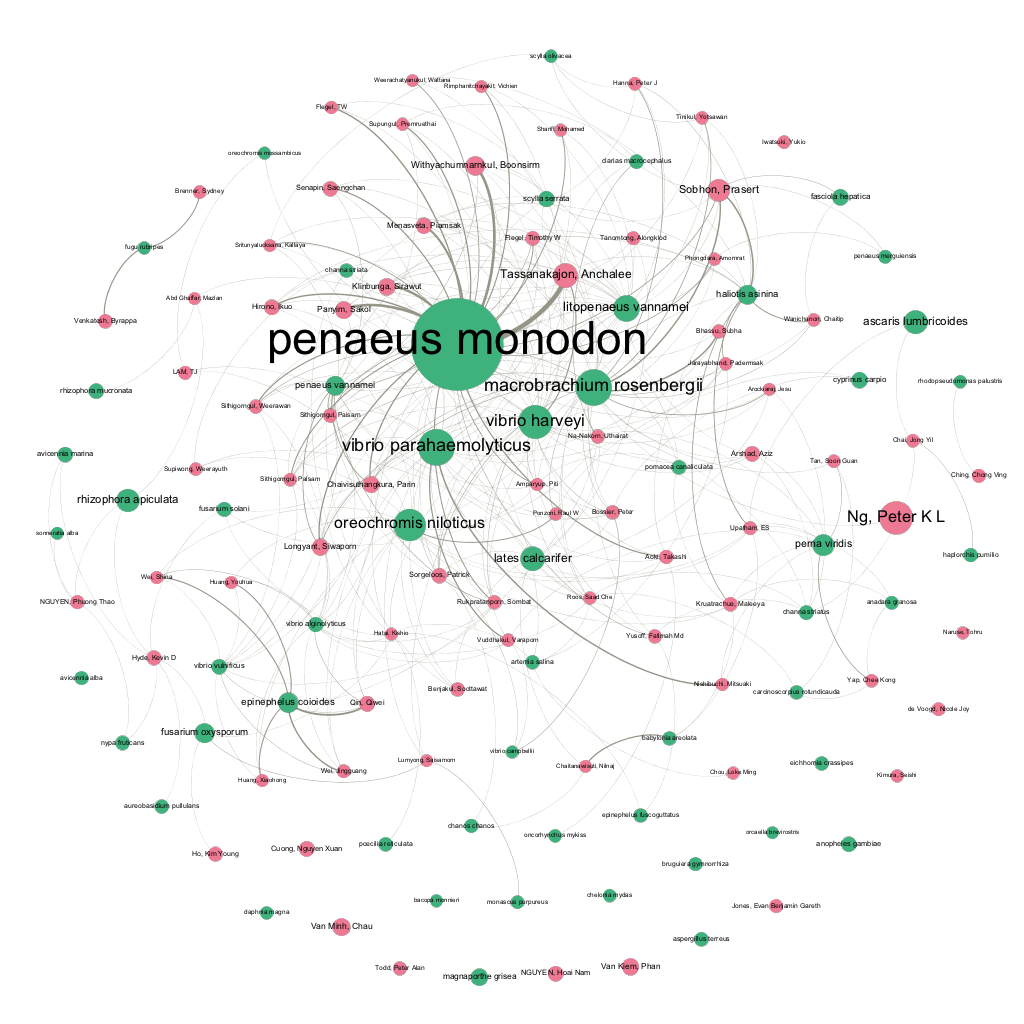
\includegraphics[width=1\linewidth]{images/asean_authors_species_directed} 

}

\caption{Researchers to Species Network in South East Asia}\label{fig:speciesresearchernetwork}
\end{figure}

In terms of the overall ranking based on publications Peter Ng Kee Lin
is the leading researcher on marine species within the ASEAN region
according to our data. However, in Figure
\ref{fig:speciesresearchernetwork} no prominent connections emerge to
species. This reflects the fact that
\href{https://lkcnhm.nus.edu.sg/dna/people/details/17}{Professor Ng Kee
Lin} is a biologist and taxonomist who has worked on a wide range of
species (notably freshwater and marine crabs)
\citep{Cai_2002, Shih_2007}. As such, viewed from a species perspective
his research is dispersed across a range of species and therefore not
immediately visible.

In contrast Figure \ref{fig:speciesresearchernetwork} reveals that
\href{http://www.bc.sc.chula.ac.th/11Anchalee.html}{Anchalee
Tassanakajon} at Chulalongkorn University in Thailand is a leading
researcher working on \emph{Peneaus mondon} with links to work on
\emph{Penaeus vannamei}, \emph{Litopenaeus vannamei}, \emph{Haliotis
asinina} (a large sea snail known as ass's ear abalone) and the main
\emph{Vibrio} pathogens
\citep{Wongteerasupaya_1995, Supungul_2004, Kaewkascholkul_2016}.
\href{http://www.sc.mahidol.ac.th/scan/old/Prasert.htm}{Professor
Prasert Sobhon in the Department of Anatomy at Mahidol University} shows
a similar pattern but with an additional focus on \emph{Macrobrachium
rosenbergii} (the giant freshwater prawn), \emph{Fasciola hepatica}
(parasitic trematodes or liver flukes) and crabs (\emph{Scylla
olivacea}, \emph{Scylla serrata})
\citep{Meeratana_2006, Duangprom_2017, Preyavichyapugdee_2008}.
\href{http://www.sc.mahidol.ac.th/scan/old/Boonsirm.htm}{Professor
Boonsirm Withyachumnarnkul at the Department of Anatomy at Mahidol
University} also specialises in \emph{Penaeus mondon} with a particular
focus on selective breeding and disease screening using DNA based
techniques \citep{Wongteerasupaya_1995} with recent work focusing on the
use of a protein extract from red seaweed to prevent hepatopancreatic
necrosis in shrimp \citep{Boonsri_2016}. In practice all three
researchers while leading distinct groups have collaborated on a number
of publications in the past
\citep{Wongteerasupaya_1995, Pongtippatee_2007, Wongteerasupaya_1997}.

This form of network analysis usefully displays the relationship between
researchers and the species they are researching. However, the
prominence of aquaculture focused research in the ASEAN research
landscape can also, as we saw in the case of Professor Ng Kee Lin,
disguise other areas of research.

Figure \ref{fig:authornetwork} revealed a research cluster focused
around Chau Van Minh at the Vietnam Academy of Science and Technology
(VAST) in Hanoi whose work, mainly conducted in collaboration with Phan
Van Kiem (now at Chungham National University in South Korea), has
included an explicit focus on pharmaceutical compounds from Marine
Natural Products
\citep{Van_Minh_2017, Quang_2011, Thao_2015, Thao_2015a}. As we saw in
Figure \ref{fig:sankeyfunding} this appears to reflect the underlying
research investments by funding organisations in Vietnam. We can gain a
clearer view of the genera involved in research directed towards
chemistry, pharmacology and biotechnology by removing dominant genera
such as Peneaus and restricting subject areas to those in chemistry,
pharmacology and biotechnology. This data is displayed in Figure
\ref{fig:pharmasankey}.

\begin{figure}

{\centering 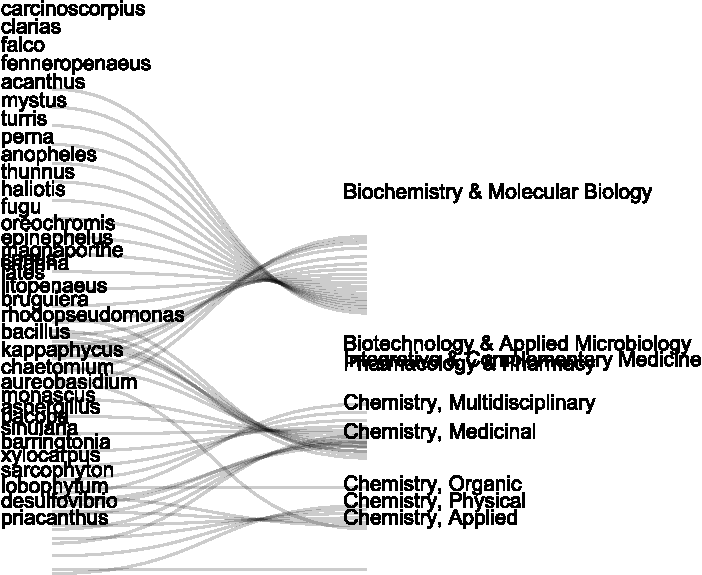
\includegraphics[width=1.2\linewidth]{asean_marine_files/figure-latex/pharmasankey-1} 

}

\caption{Pharmaceutical Focused Research for Marine Genetic Resources in the ASEAN region}\label{fig:pharmasankey}
\end{figure}

The top genus emerging in this area are sea snails (gastropods) in the
Conus genera with a total of 37 publications in the ASEAN data. Top
cited research on Conus includes collaborative research between the
University of the Philippines and the University of Utah in the 1990s to
identify a Novel Alpha Conotoxin and Omega Conotoxin from \emph{Conus
striatus} Venom, along with other research on a delta conotoxin from
\emph{Conus gloriamaris} \citep{Ramilo_1992, Shon_1994}. More recent
work at the University of the Philippines with the University of Utah
has involved characterisation of the complete mitochondrial genome of
\emph{Conus tribblei} and the structural features of conopeptide genes
focusing on gene encoded peptide toxins
\citep{Barghi_2015, Barghi_2015}. In Vietnam, members of the Conus genus
have also been a focus of research between the University of Nha Trang
and CNRS in France concentrating on the identification of novel venom
compounds including the use of novel proteomic approaches
\citep{Nguyen_2013, Nguyen_2014, Nguyen_2014a, Nguyen_2014b}

A second important genus in research directed towards pharmaceuticals
and similar products are members of the Channa genus or snakehead fish
which includes a range of species found in brackish or freshwater.
Research at the University Putra Malaysia has focused on comparative
analysis of the protein content of Channa species with a focus on levels
of DHA as an explanation for their use in traditional knowledge
practices for reducing pain, inflammation and wound healing in Malaysia
\citep{Zuraini_2006}. More recent research by the University Putra
Malaysia has focused on the antidepressant like effects of a lipid
extract from \emph{Channa striatus} and investigation of wound healing
\citep[Abdul\_Shukkoor\_2016;][]{Baie_2000, Mohamad_Isa_2016}.

As this brief summary of research in two genera suggests, while the
marine research data is dominated by fisheries and aquaculture related
research there is also an important strand of research in Chemistry and
Biochemistry focusing on the medical properties of organisms and linking
through to using traditional knowledge as a lead for research.

\hypertarget{conclusion-1}{%
\subsection{Conclusion}\label{conclusion-1}}

In this section we have mapped and explored the landscape of over 6000
publications on marine genetic resources for the ASEAN region involving
3,685 marine species. The global research network for research on ASEAN
marine species has involved approximately 17,625 researchers from nearly
4,000 organisations distributed in 136 countries. As we have seen in
this section research activity for marine species in the ASEAN region is
growing in the majority of countries. Research activity ranges from
basic taxonomic and ecological research to a major concentration of
research effort in the aquaculture sector and important concentrations
of research in marine natural products directed towards biotechnology
and pharmaceuticals. We have also seen that funding for marine research
in the ASEAN region is critically dependent on national research funding
agencies and an important network of international funding agencies from
Japan, China, the United States and Europe who support collaborative
research with researchers within and outside the region. In the next
section we turn to analysis of the available data on patent activity
involving marine species in the ASEAN region with a particular focus on
identifying patent activity by researchers from the region.

\hypertarget{patent}{%
\chapter{Patent Activity for Marine Genetic Resources in the ASEAN
Region}\label{patent}}

In this section we focus on patent activity involving researchers and
marine genetic resources in the ASEAN region. Our aim is to understand
the nature of patent activity exhibited by researchers from within the
region working on marine genetic resources and to situate their research
in the wider context of research and development for marine genetic
resources.

We begin the section with a brief overview of patent activity in the
region and consideration of the challenges involved in examining patent
activity in ASEAN countries. We then move into analysis of patent
activity that includes a marine species originating from or making
reference to an ASEAN country.

\hypertarget{patent-overview}{%
\subsection{Patent Overview}\label{patent-overview}}

There are two primary sources for global patent data for statistical
purposes. The first of these is the European Patent Office World Patent
Statistical Database (known as PATSTAT) and the second are commercial
databases, such as Derwent Innovation from Clarivate Analytics. For
statistical research PATSAT is preferred as the international baseline.
However, our research exposed significant problems with the use of
PATSTAT in the case of ASEAN countries.

We initiated research with PATSTAT (Autumn 2016 edition) by identifying:

\begin{enumerate}
\def\labelenumi{\alph{enumi})}
\tightlist
\item
  patent applications where an ASEAN country was the application
  authority (210,972 records). This data captures priority filings from
  the ASEAN region even where they are not published or published
  outside the region.
\item
  patent applications where an ASEAN country is the publication
  authority (173,461 records).
\item
  patent applications anywhere in the world where an applicant or
  inventor is listed from an ASEAN country (109,744 records).
\end{enumerate}

These documents may contain duplicates and were deduplicated to 299,830
applications. This data is presented in the left panel of Figure
\ref{fig:coverage}.

It is immediately clear from Figure \ref{fig:coverage} that the data is
irregular across countries. For Indonesia, PATSTAT data is limited to
information from the late 1990s and early 2000s. The Philippines
displays a pattern of an early peak in the 1990s followed by a long
trough until the late 2000s while information for Thailand and Vietnam
is very limited and is absent for Brunei, Cambodia and Laos. At first
sight the data for Malaysia and Singapore appears to be more consistent
however, the presence of major peaks or troughs is typically a sign of
missing or incomplete data.

\begin{figure}

{\centering 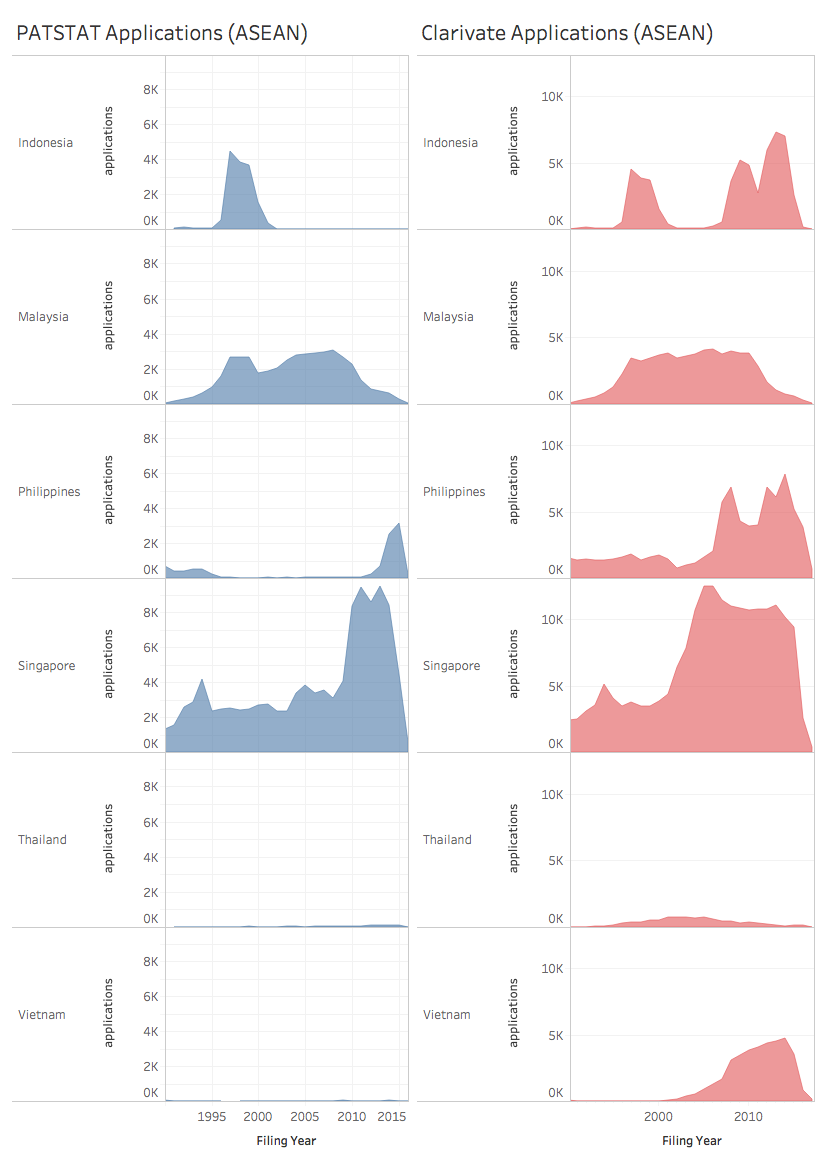
\includegraphics[width=1\linewidth]{images/patstat_and_clarivate} 

}

\caption{PATSTAT and Derwent Innovation coverage for ASEAN countries}\label{fig:coverage}
\end{figure}

To test levels of data completeness, the same query was performed using
Derwent Innovation from Clarivate Analytics (formerly Thomson
Innovation). Derwent Innovation includes the full text collections for
the majority of ASEAN countries (Malaysia, Singapore, Vietnam, Thailand
and the Philippines). Datasets were downloaded and deduplicated to
461,380 distinct patent applications. Trends based on Derwent Innovation
data are displayed in the right hand panel of Figure \ref{fig:coverage}.
This approach yielded an additional 162,000 applications and had a
dramatic impact on the availability of data from ASEAN countries. Data
for Singapore radically improves for recent years with improvements in
data for Thailand on a more modest level. Data for Vietnam, again for
recent years, also improves markedly.

Comparison of the data between PATSTAT and Derwent Innovation exposes
two problems. The first of these in the case of PATSTAT is the problem
of data availability. Put simply, the ASEAN collections are effectively
not present in PATSTAT data (Autumn 2016). The second is the problem of
data completeness. While Derwent Innovation radically improves coverage,
the presence of peaks and troughs also suggests a lack of data
completeness. Presumably, this reflects the lack of availability of
patent documents in electronic form for earlier years. It is also likely
that for later years there are lag times in the availability of
electronic records.

The practical consequence of these issues is that data for ASEAN
countries is presently incomplete. We are therefore obliged to work
within the constraints of the available data. However, we would note
that the availability and completeness of the patent collections for the
ASEAN region will also affect the ability of ASEAN countries to fully
understand and assess the economic significance of patent activity for
their country and region.

\hypertarget{search-strategy}{%
\subsection{Search Strategy}\label{search-strategy}}

The aim of our search strategy was to capture two areas of patent
activity:

\begin{enumerate}
\def\labelenumi{\arabic{enumi}.}
\tightlist
\item
  Patent activity for marine genetic resources originating from within
  the region
\item
  Patent activity for marine genetic resources that could involve marine
  genetic resources collected from the region.
\end{enumerate}

This aim required us to examine activity from within the region and
wider activity. To achieve this we used a three part methodology.

\begin{enumerate}
\def\labelenumi{\alph{enumi})}
\item
  Text mining the titles, abstracts and claims of Clarivate records from
  the ASEAN collection for binomial species names from the World
  Register of Marine Species (WoRMS) in VantagePoint. This identified an
  initial 730 first filings for 302 marine species.
\item
  Combining the data with existing data on marine patent activity within
  the ABSPAT index linked to ASEAN countries. The ABSPAT index consists
  of 6.5 million sentences from patent documents from the full texts of
  the EPO, USPTO and PCT collections until 2013 that contain a country
  name and a separate table containing 21.4 million sentences containing
  a species names. The ASEAN country names were identified in the
  country table and then cross referenced with the species table
  yielding 15,376 documents containing a species name and an ASEAN
  country name. This data was deduplicated to 6,521 first filings. Text
  mining of this set for marine species names revealed 2,033 first
  filings containing an ASEAN country name and a marine species.
\item
  A keyword based search strategy. We aimed to capture additional
  records outside the Clarivate search of ASEAN jurisdictions and the
  historic ABSPAT data for the US, EP and WO. As the WoRMS data consists
  of over 390,000 marine species names a search strategy was required
  that would capture those names. This strategy was advanced by
  developing a query that captured species names without directly using
  a species name. Experimentation with the texts of the 6,521 first
  filings for the ASEAN region mentioned above from ABSPAT revealed that
  the following search strategy captured 98\% of documents in the
  dataset.
\end{enumerate}

\begin{quote}
``species'' OR ``genus'' OR ``family'' OR ``order'' OR ``phylum'' OR
``class'' OR ``kingdom'' OR ``tribe'' OR ``DNA'' OR ``nucleic'' OR
``nucleotide'' OR ``amino'' OR ``polypeptide'' OR ``sequence'' OR ``SEQ
ID'' OR ``protein'' OR ``proteins'' OR ``peptides'' OR ``peptide'' OR
``enzyme'' OR ``enzymes'' OR ``plant'' OR ``plants'' OR ``animal'' OR
``animals'' OR ``mammal'' OR ``mammals'' OR ``mammalian'' OR
``bacteria'' OR ``protozoa'' OR ``virus'' OR ``viruses'' OR ``fungi'' OR
``animalia'' OR ``archaea'' OR ``chromista'' OR ``chromist'' OR
``chromists'' OR ``protista'' OR ``protist'' OR ``protists'' OR
``plantae'' OR ``eukaryotes'' OR ``eukaryotes'' OR ``eukaryote'' OR
``prokarya'' OR ``prokaryote'' OR ``prokaryotes'' OR ``microorganism''
OR ``microorganisms'' OR ``organism'' OR ``organisms'' OR ``cell'' OR
``cells'' OR ``gene'' OR ``genes'' OR ``genetic'' OR ``viral'' OR
``biological'' OR ``biology'' OR ``strain'' or ``strains'' or
``variety'' or ``varieties''
\end{quote}

Beyond these terms the addition of new terms produced diminishing
returns. If used across the full texts of the Derwent Innovation
collection, the above search query produced 30 million publications.
However, patent applicants typically include references to species and
related terms in the Title, Abstract or Claims of documents. As our aim
was to capture documents for marine species that may have originated
from the region we therefore adopted a strategy of:

\begin{enumerate}
\def\labelenumi{\alph{enumi})}
\tightlist
\item
  searching for ASEAN country names in the description section of the
  patent documents.
\item
  searching the title, abstracts and claims for the species related
  terms
\end{enumerate}

The search query was run in two sets (1990-2009 and 2010-2017) focusing
on the US, EP, JP and WO and the ASEAN jurisdictions.

\begin{quote}
(PY\textgreater{}=(1990) AND PY\textless{}=(2009)) AND DSC=(``brunei''
or ``cambodia'' or ``indonesia'' or ``laos'' or ``lao'' or ``malaysia''
or ``philippines'' or ``myanmar'' or ``burma'' or ``singapore'' or
``thailand'' or ``vietnam'') AND CTB=(``species'' OR ``genus'' OR
``family'' OR ``order'' OR ``phylum'' OR ``class'' OR ``kingdom'' OR
``tribe'' OR ``DNA'' OR ``nucleic'' OR ``nucleotide'' OR ``amino'' OR
``polypeptide'' OR ``sequence'' OR ``SEQ ID'' OR ``protein'' OR
``proteins'' OR ``peptides'' OR ``peptide'' OR ``enzyme'' OR ``enzymes''
OR ``plant'' OR ``plants'' OR ``animal'' OR ``animals'' OR ``mammal'' OR
``mammals'' OR ``mammalian'' OR ``bacteria'' OR ``protozoa'' OR
``virus'' OR ``viruses'' OR ``fungi'' OR ``animalia'' OR ``archaea'' OR
``chromista'' OR ``chromist'' OR ``chromists'' OR ``protista'' OR
``protist'' OR ``protists'' OR ``plantae'' OR ``eukaryotes'' OR
``eukaryotes'' OR ``eukaryote'' OR ``prokarya'' OR ``prokaryote'' OR
``prokaryotes'' OR ``microorganism'' OR ``microorganisms'' OR
``organism'' OR ``organisms'' OR ``cell'' OR ``cells'' OR ``gene'' OR
``genes'' OR ``genetic'' OR ``viral'' OR ``biological'' OR ``biology''
OR ``strain'' or ``strains'' or ``variety'' or ``varieties'' or ``common
name'');
\end{quote}

This dataset consisted of a raw 73,164 documents that were deduplicated
to the first application numbers to 38,120 first filings. The available
full texts for these documents were downloaded and text mined for marine
species names using a tidy text mining approach \citep{R-tidytext}.

In total, this approach yielded 5,742 applications based in 3,587 first
filings either originating from the ASEAN region or referencing an ASEAN
country within the text and containing a marine species. These documents
were text mined by document section (title, abstract, description and
claims) in R using a tidy text mining approach as the basis for the
analysis in this section.

An important constraint with this data is that while the documents
contain a reference both to a marine species and to an ASEAN country,
the reference to the ASEAN country may occur for reasons that are not
related to the origin of the marine species. For example, a country may
be referenced as the source of a commercial supplier of material. As
such, while it is a precondition of the data that it either originate
from an ASEAN country and contain a marine species or reference an ASEAN
species and a marine species, there is a fuzzy element to the outlines
of this data.

\hypertarget{an-overview-of-filing-trends}{%
\subsection{An Overview of Filing
Trends}\label{an-overview-of-filing-trends}}

Figure \ref{fig:firstfilings} presents an overview of the first filings
of patent applications involving marine genetic resources linked to the
ASEAN region. Trends in first filings refer to the original filing of an
application (anywhere in the world) and displays a characteristic
\emph{data cliff} the closer we move towards the present day. This
reflects the lag time between the first filing of a patent application
and its publication (typically 24 months after filing).

\begin{figure}

{\centering 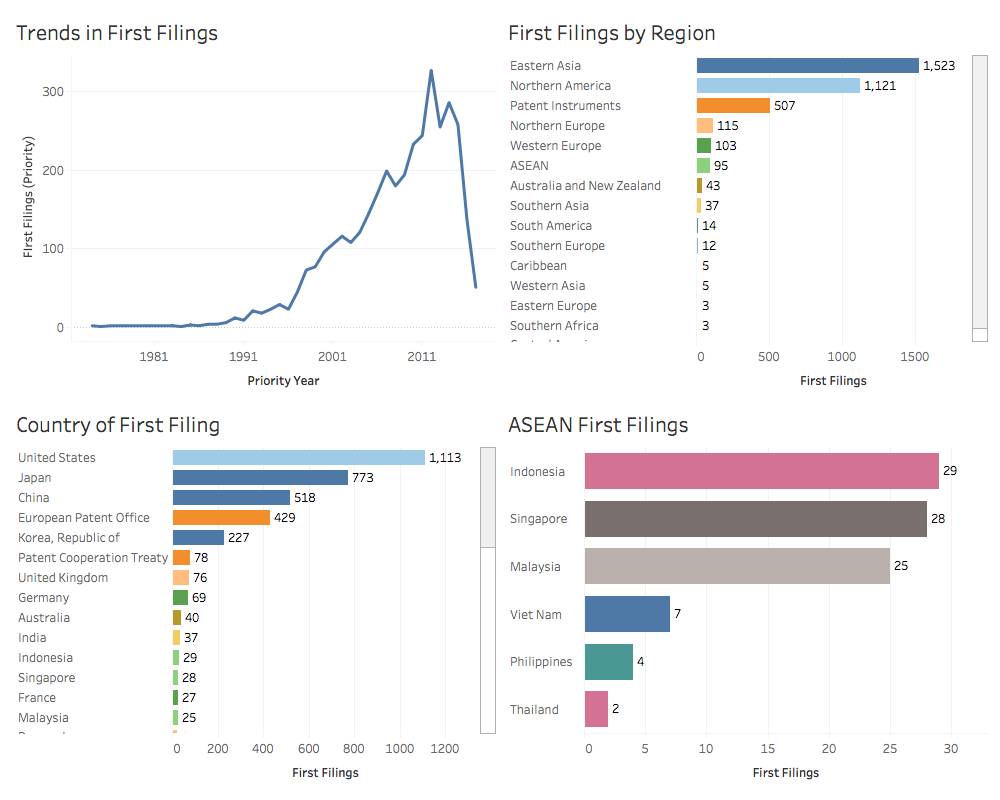
\includegraphics[width=1\linewidth]{images-patents/first_filings} 

}

\caption{Trends in First Filings for Marine Species linked to the ASEAN region}\label{fig:firstfilings}
\end{figure}

The panel on first filings by region aggregates the first filings
displayed by country using the United Nations regional division and
reveals that Eastern Asia (Japan, China and South Korea) account for the
majority of first filings followed by North America (dominated by
filings in the United States). Patent instruments (notably the European
Patent Convention through the European Patent Office) and the Patent
Cooperation Treaty rank third and will reflect an EP or PCT first filing
strategy on the part of applicants.\footnote{United Nations Statistical
  Division \href{https://unstats.un.org/unsd/methodology/m49/}{Standard
  country or area codes for statistical use (M49)}}

Within the ASEAN region filings are evenly spread between Indonesia,
Singapore and Malaysia, with a lower level of first filings from
Vietnam, the Philippines and Thailand. As we will see below, in practice
activity from researchers in ASEAN countries is higher than is suggested
by reduction to the earliest filings.

\hypertarget{patent-family-trends}{%
\subsection{Patent Family Trends}\label{patent-family-trends}}

The first filings of patent applications lead to follow on applications
and grants (family members) within the country of filing and, using
international instruments, in other countries. Patent Family analysis
allows us to identify the markets where applicants are seeking
protection. Figure \ref{fig:families} displays follow on filings around
the world by individual country and summarises the data by major United
Nations region. The data on family members has been adjusted to remove
search reports from the data for the European Patent Office and the
Patent Cooperation Treaty to avoid counting purely administrative
documents.

\begin{figure}

{\centering 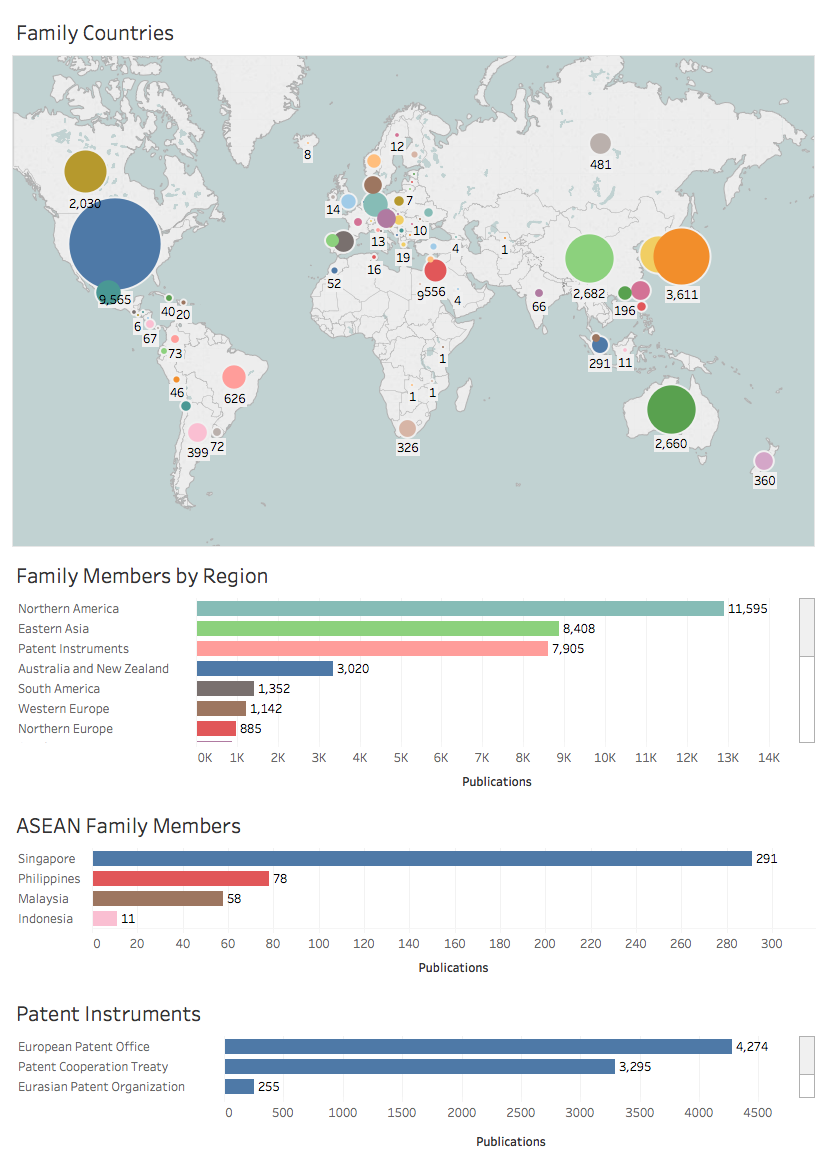
\includegraphics[width=1\linewidth]{images-patents/families} 

}

\caption{Overview of Patent Family Members world wide for Marine Species linked to the ASEAN region}\label{fig:families}
\end{figure}

Figure \ref{fig:families} demonstrates that demand for patent rights is
highest within North America followed by Eastern Asia (China, South
Korea and Japan) with regional and international patent instruments
playing an important role in enabling the pursuit of protection in
multiple markets. The ASEAN region itself is not a major focus of demand
for patent rights based on the available data.

Figure \ref{fig:familyregiontrends} displays the available data on
trends in demand for patent rights, broken down by the main regions for
ease of visibility. In \emph{Figure 4.5} a major spike is immediately
visible for North America that starts at the end of 2001 and peaks in
2003. This is an artefact from the transition in the United States from
the publication of patent grants prior to 2001 to the publication of
both applications and grants after 2001 leading to an apparent, rather
than real, surge in activity.

\begin{figure}

{\centering 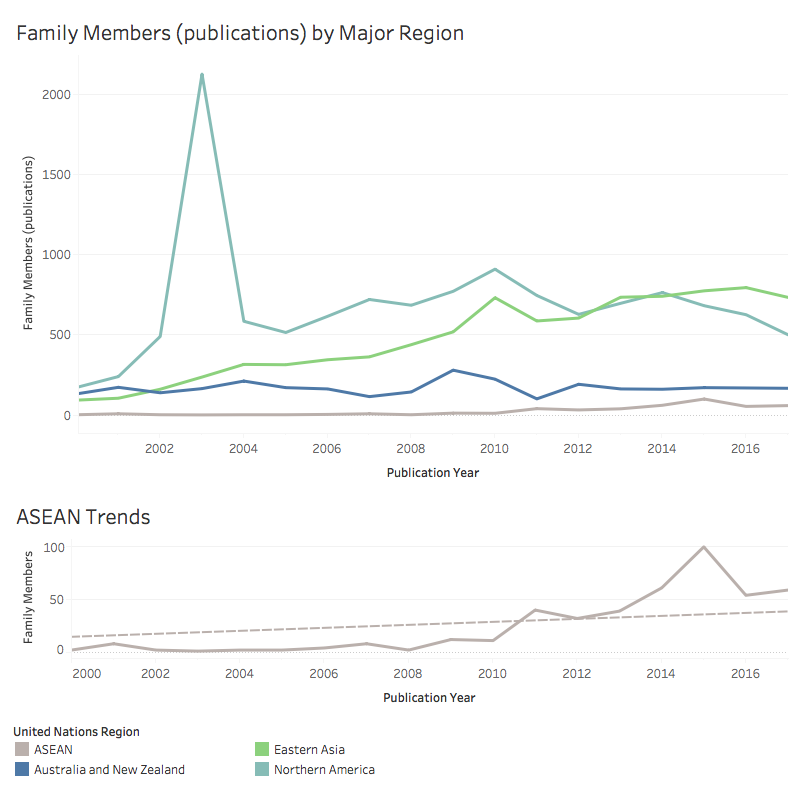
\includegraphics[width=1\linewidth]{images-patents/family_trends_region} 

}

\caption{Trends in Family Publications by Major Region for Marine Species linked to the ASEAN region}\label{fig:familyregiontrends}
\end{figure}

We can also observe that activity for the ASEAN region in the lower
panel of Figure \ref{fig:familyregiontrends} is at a significantly lower
level, across the period 2000-2017 and peaking with 100 records in 2015.
As this suggests, demand for patent rights involving marine genetic
resources that can be linked to the ASEAN region is best classified as
emergent.

\hypertarget{top-species}{%
\subsection{Top Species}\label{top-species}}

A single patent document may contain a range of species. Figure
\ref{fig:patentspecies} presents an overview of the top species by
counts of applications and species counts.

\begin{figure}

{\centering 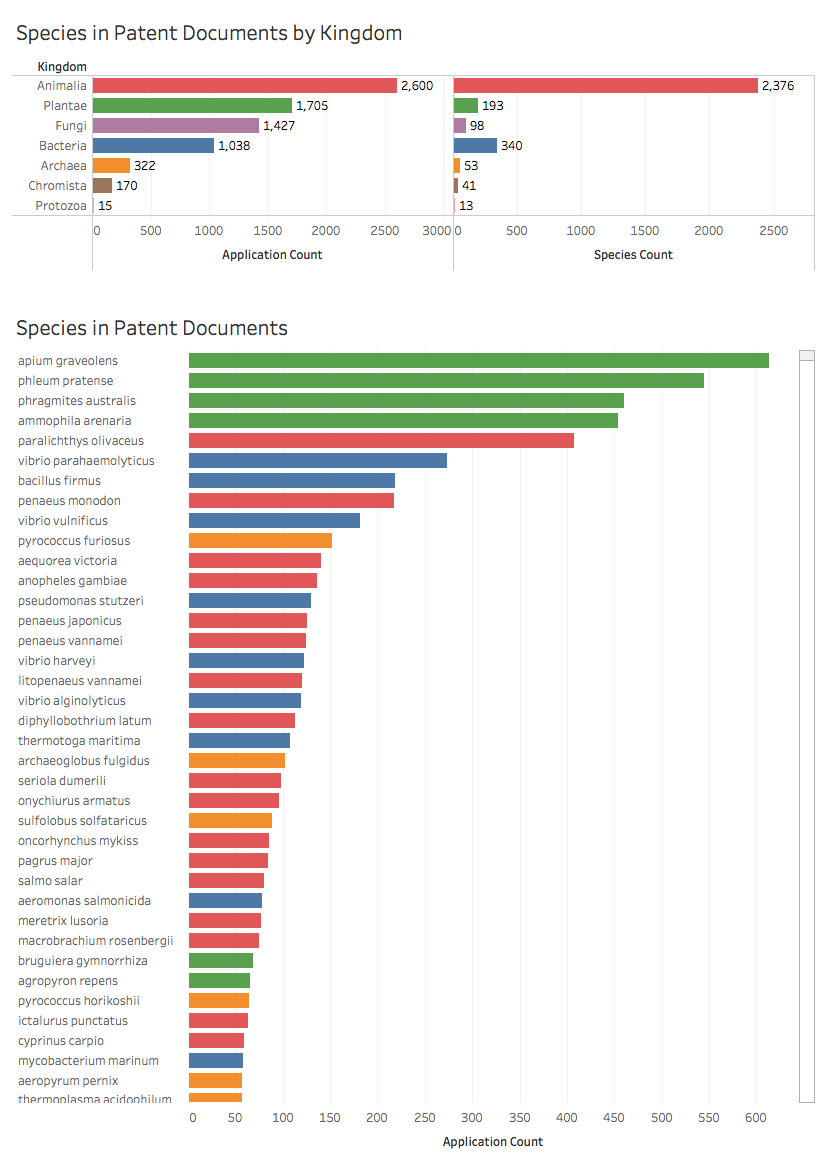
\includegraphics[width=1\linewidth]{images-patents/patent_species_dashboard} 

}

\caption{Summary Marine Species linked to ASEAN countries in Patent Data}\label{fig:patentspecies}
\end{figure}

In total 3,114 species from the World Register of Marine Species
appeared in the patent documents. We have excluded species where they
were classified as terrestrial, or where environment information was not
available. We have also excluded Fungi from the display of species as
they are not normally sourced from a marine environment (see below).

Figure \ref{fig:patentspecies} illustrates that a number of the top
species in the overall marine data are plants. This also illustrates
some of the challenges involved in identifying marine species that cross
environments. \emph{Apium graveolens} is better known as Celery and is
included within the marine data because it was originally a marsh plant
that can grow in salt water conditions and features in patent activity
for herbicide resistance (JP2013046624A). \emph{Phleum pratense} is a
widespread invasive grass that can be found in brackish conditions and
appears in patent activity for control of plant pathogens
(IN200800137P1). \emph{Phragmites australis} is a perennial wetland
grass with patent claims that focus on the use of the species, among
others, as feedstock in methods for producing cellulose pulp
(WO2017178849A1). \emph{Ammophila arenaria} is commonly known as beach
grass and typically appears as a passing reference in the description of
patent activity focusing on genetic engineering to increase yields in a
wide range of plants, rather than as the focus of an invention
(EP2316956A2).

As noted in the discussion of the scientific landscape, fungi such as
\emph{Fusarium oxysporum}, \emph{Aureobasidium pullans}, \emph{Fusarium
solani}, \emph{Aspergillus terreus} and \emph{Alternaria alternata}
among other fungi in the data are extremely widespread in soils and
other habitats and patent activity is not typically directly linked with
these organisms from a marine environment. We have therefore excluded
fungi from the display of species in Figure \ref{fig:patentspecies}
while noting that marine fungi are an increasing focus of interest in
the wider scientific literature \citep[see for example,][]{Kim_2012}. It
is therefore important not to second guess categories of organism that
are of interest in the marine environment.

Figure \ref{fig:patentspeciestechnology} presents the data above in
terms of the technology areas that are the focus of activity by the
number of species and the number of applications. The definition of
technology areas is based on the use of Subclasses from the
International Patent Classification. The International Patent
Classification is used by patent offices worldwide to classify the
technical content of patent documents and consists of alphanumeric
codes. Because the descriptions associated with a code may be very long
the Subclasses have been edited to short versions for ease of
presentation.

\begin{figure}

{\centering 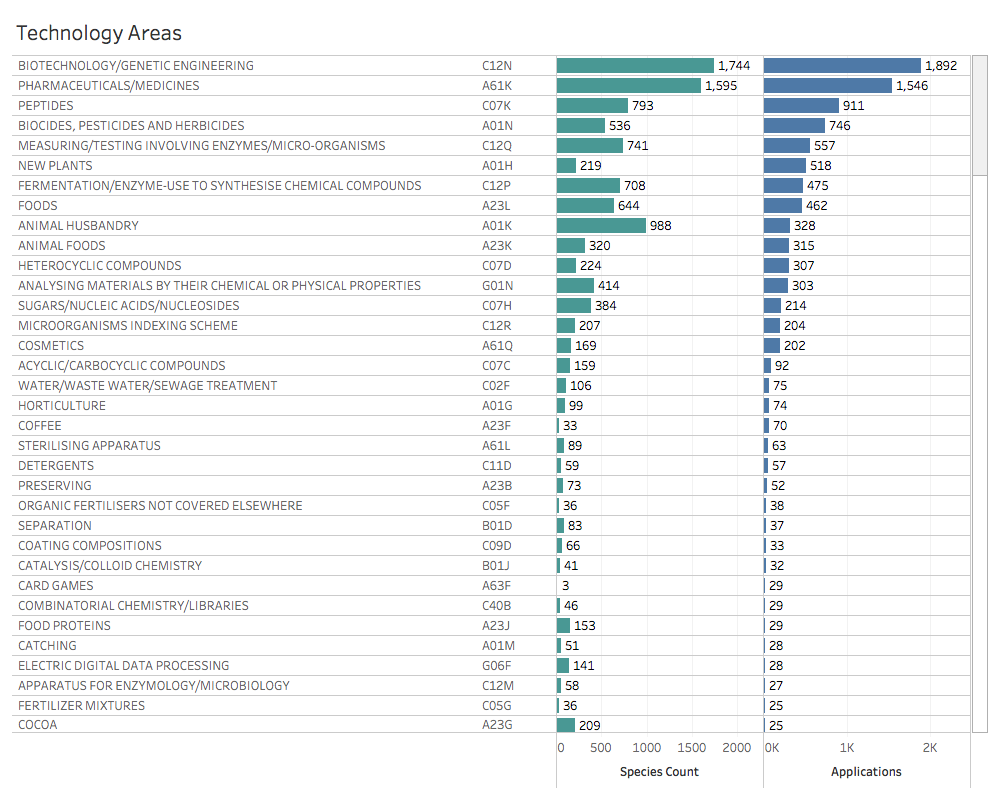
\includegraphics[width=1\linewidth]{images-patents/technology_areas_species} 

}

\caption{Summary of Marine Species linked to ASEAN countries in Patent Data}\label{fig:patentspeciestechnology}
\end{figure}

Figure \ref{fig:patentspeciestechnology} reveals that species and
applications across the dataset are concentrated in the fields of
biotechnology and pharmaceuticals. However, as we will see in more
detail below fields such as aquaculture are also prevalent but dispersed
across the fields of Animal Husbandry (A01K), Animal Foods (A23K) and
Water/Waste Water/Sewage Treatment (C02F).

\hypertarget{asean-researchers-as-inventors}{%
\subsection{ASEAN Researchers as
Inventors}\label{asean-researchers-as-inventors}}

In the previous section we examined the research activities of the
approximately 17,625 researchers involved in research on marine species
linked to the ASEAN region. We now focus in on the analysis of those
researchers within the scientific literature who are also inventors.

In order to identify researchers who are also inventors we combined the
names of the 17,625 researchers from the scientific literature together
with the inventor name field containing 9,382 cleaned names. Name
matches and close name matches were then examined against the criteria
of the appearance of co-authors who are also inventors, author
affiliation and applicant name matches and matches on species names
between the scientific and patent literature linked to an author name.
Where one or more of these criteria were met the author was classified
as an author inventor.

In total we identified 290 authors who are also inventors in patent
applications involving marine genetic resources. Taken together author
inventors accounted for 369 applications that referenced 446 marine
species.

Figure \ref{fig:authorinventorspecies} displays the rankings for species
appearing in patent documents based on counts of applications. The
smaller panels display details for certain kingdoms that would otherwise
be hidden.

\begin{figure}

{\centering 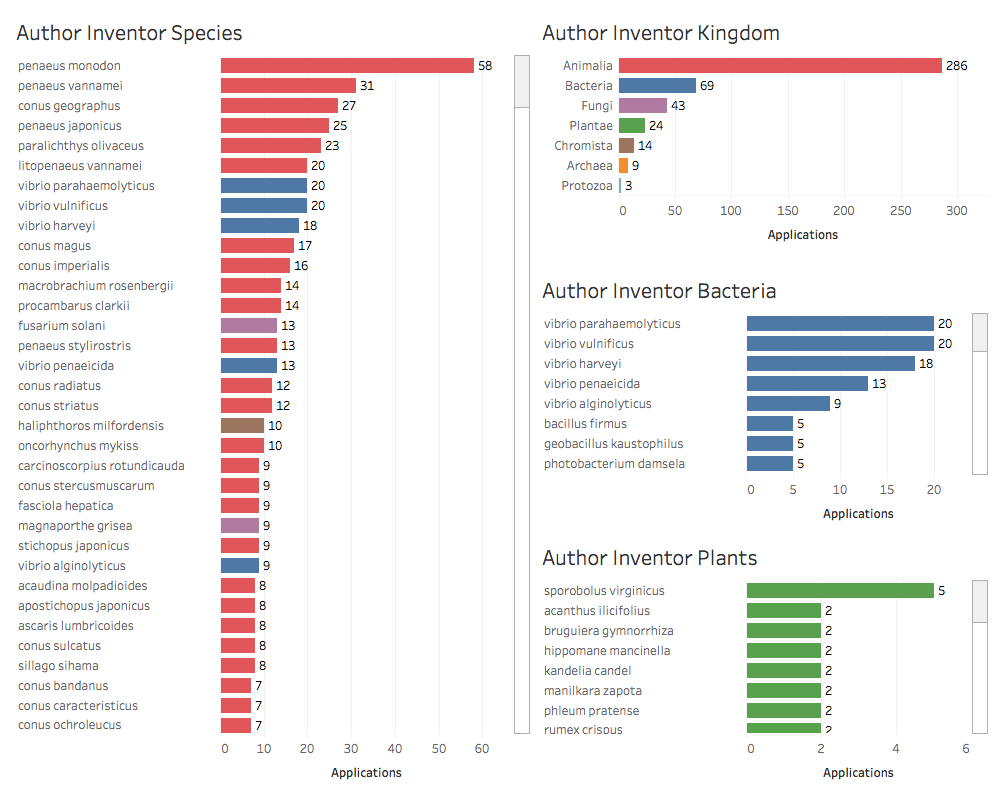
\includegraphics[width=1\linewidth]{images-patents/author_inventor_species_dashboard} 

}

\caption{Summary of Marine Species linked to ASEAN countries in Patent Data}\label{fig:authorinventorspecies}
\end{figure}

In considering Figure \ref{fig:authorinventorspecies} we can readily see
that animal species are dominant with shrimp genera (Penaeus) in the
aquaculture sector dominating the rankings with \emph{Paralichthys
olivaceus} or Japanese halibut also appearing high in these rankings.
Bacteria in the Vibrio genus, again reflecting the aquaculture sector,
dominate the rankings for bacteria. \emph{Bacillus thermus}, a high
temperature and alkaline tolerant bacterium, among others such as
\emph{Geobacillus kaustophilus} (a deep sea bacterium reportedly
isolated from the Mariana Trench)\footnote{\url{https://microbewiki.kenyon.edu/index.php/Geobacillus_kaustophilus}}
and \emph{Photobacterium damsela} (associated with Pastereullosis in
fish) appear in a list of 35 bacteria in the patent documents.

In the case of plants, they typically appear in the description section
of patent documents within the dataset rather than as the focus of the
invention. \emph{Sporobolus virginicus} is a shoreline couch grass,
\emph{Bruguiera gymnorhiza} is the black mangrove, \emph{Hippomane
mancinella} is a coastal tree that is often found in association with
mangroves (WO2013137822A1), \emph{Kandelia candel} is a mangrove native
to South East Asia and \emph{Manilkara zapota} is a widely grown coastal
fruit tree. \emph{Phleum pratense} is a widely distributed coastal
grass, and \emph{Rumex crispus}, or yellow dock, is a widespread plant
with a coastal sub species.

Figure \ref{fig:authorinventordash} displays a summary for researchers
as inventors based on counts of the number of patent applications
associated with a researcher.

\begin{figure}

{\centering 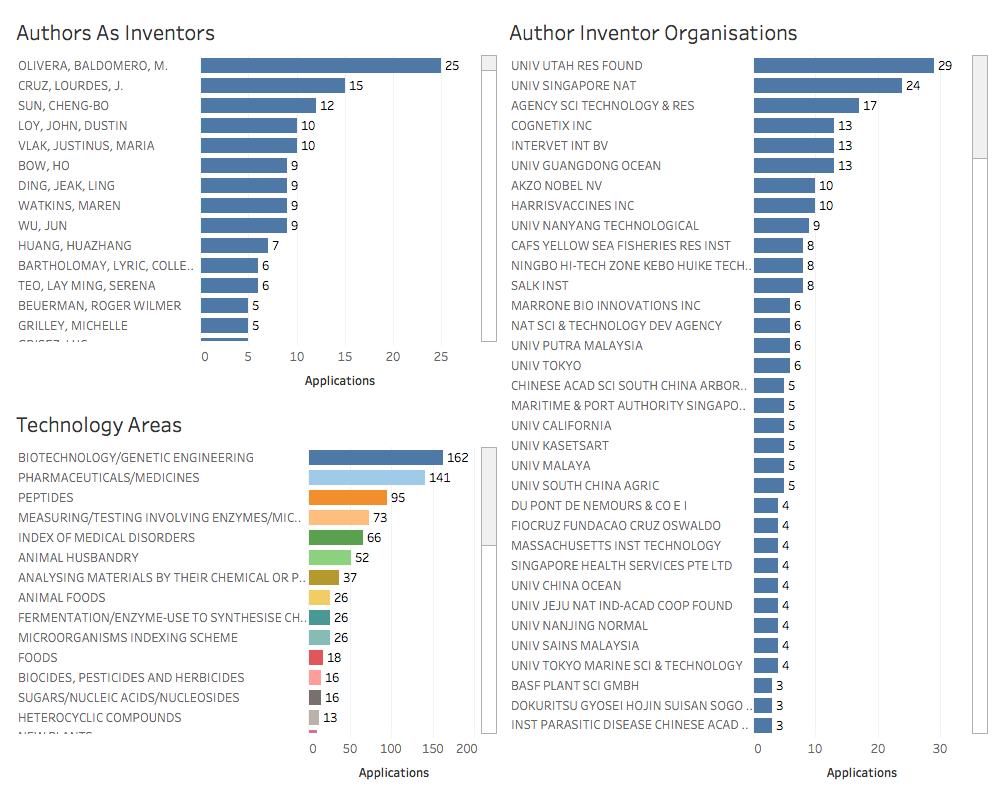
\includegraphics[width=1\linewidth]{images-patents/author_inventor_dashboard} 

}

\caption{A summary of author-inventors by number of applications, organisations and technology areas}\label{fig:authorinventordash}
\end{figure}

We can clearly see in Figure \ref{fig:authorinventordash} that while
overall applications are low, there are clear leaders with organisations
representing a mixture of universities, government research
organisations and private companies across a number of countries
including the United States, China and Japan.

In the analysis of the scientific literature we approached the data in
terms of networks of authors and organisations. We will adopt the same
approach for the analysis of the patent data. Note that collaboration
networks in patent data, notably between organisations, are typically
sparser than in the case of the scientific literature.

Figure \ref{fig:authorinventornet} displays the network clusters for
author inventors where node size is based on the number of applications
associated with a researcher. Figure \ref{fig:authorapplicantnet}
displays the network of organisations (applicants) associated with the
applications.

\begin{figure}

{\centering 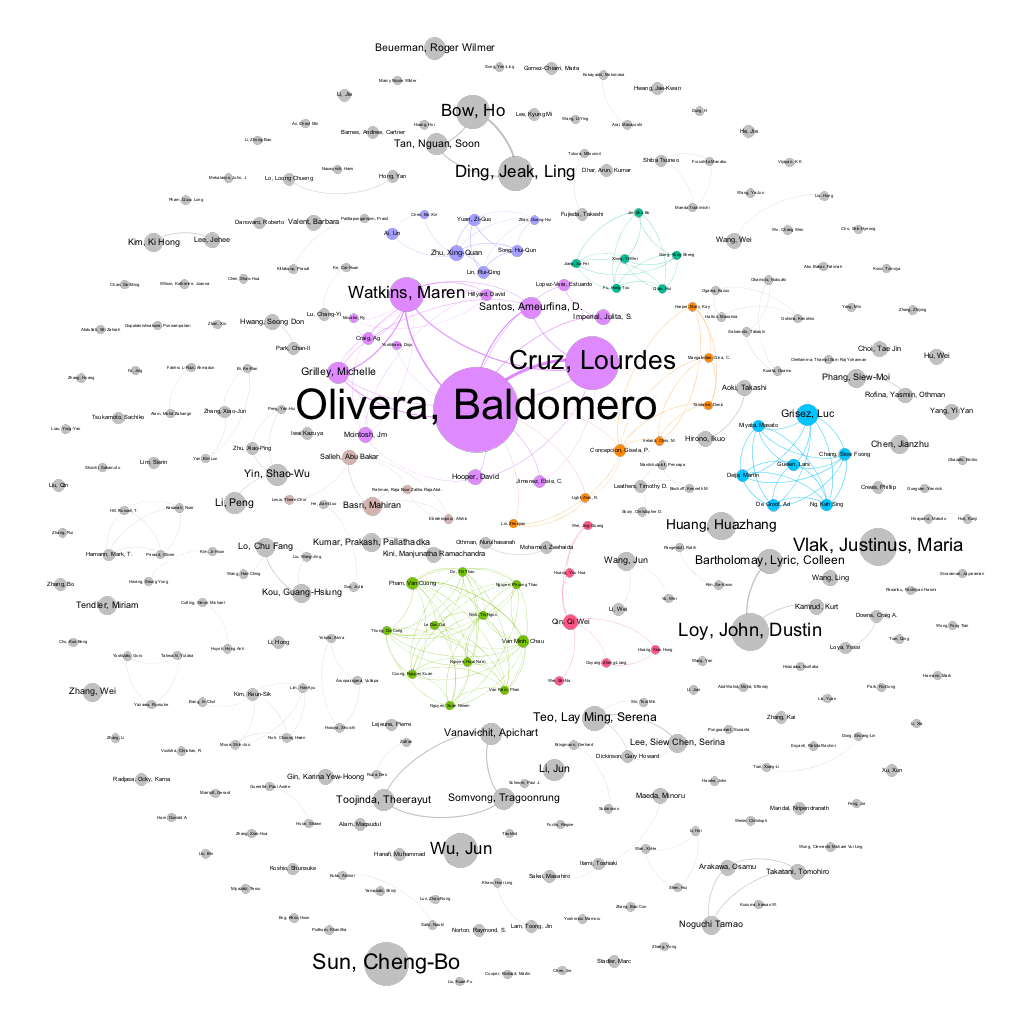
\includegraphics[width=1\linewidth]{images-patents/author_inventor_network} 

}

\caption{Author-Inventor Networks for Marine Genetic Resources in the ASEAN Region}\label{fig:authorinventornet}
\end{figure}

\begin{figure}

{\centering 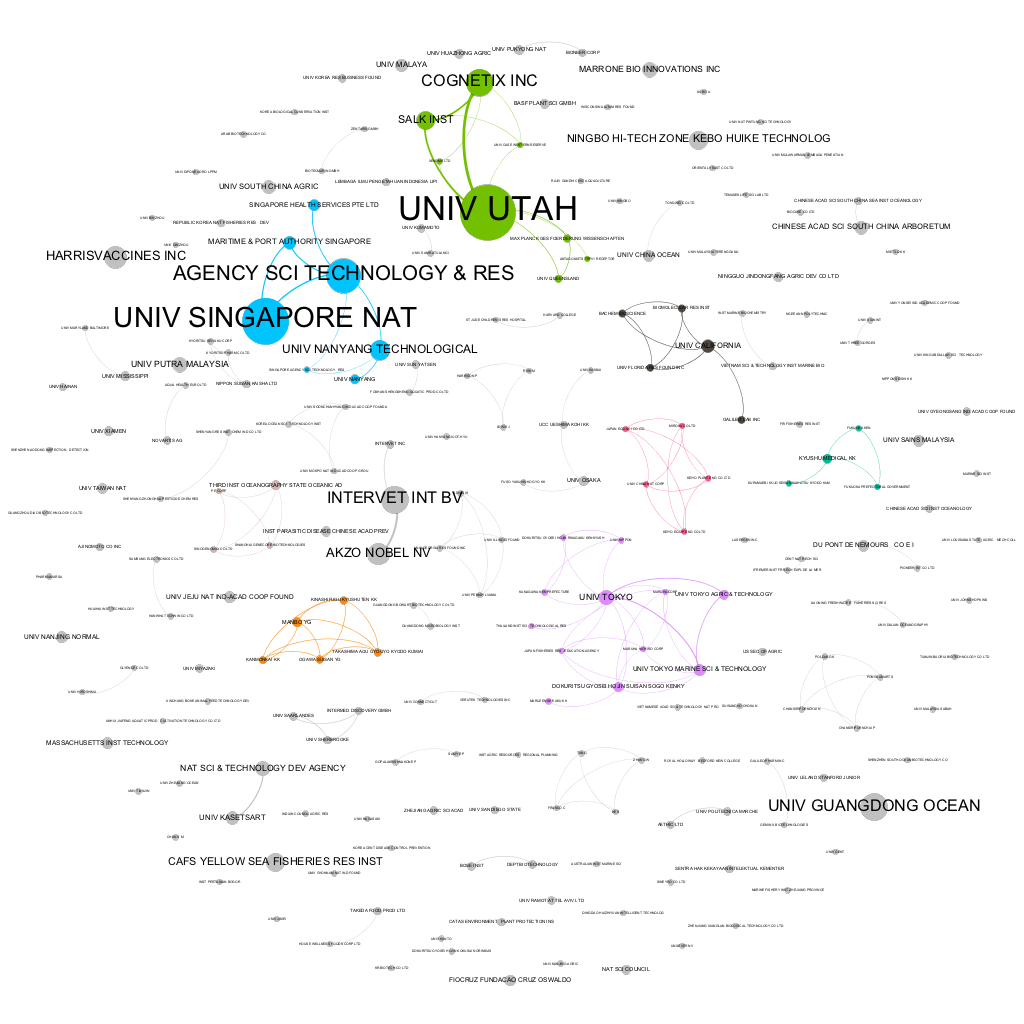
\includegraphics[width=1\linewidth]{images-patents/author_inventor_applicants_network} 

}

\caption{Author-Inventor Applicant Networks for Marine Genetic Resources in the ASEAN Region}\label{fig:authorapplicantnet}
\end{figure}

Figure \ref{fig:authorinventornet} reveals clear clusters of researchers
who also appear as inventors on patent applications involving marine
species. As we will see below, in practice the data for researchers
reveals three basic sets of circumstances where researchers submit
patent applications.

\begin{enumerate}
\def\labelenumi{\alph{enumi})}
\tightlist
\item
  Cases where a researcher has a pre-existing patent portfolio (that may
  be in a different subject area such as plant biotechnology) who then
  joins a research collaboration in the new area;
\item
  Cases where researchers jointly submit patent applications arising
  from their joint research;
\item
  Cases where members of a research group go on to form a sub-cluster
  and file patent applications arising from their research;
\end{enumerate}

In the case of data on applicants we can see that as expected,
applicants are typically sole applicants. However, we can see cases of
collaboration in patent filings around the National University of
Singapore, the University of Utah and the University of Tokyo. In other
cases such as Guangdong Ocean University in China, a significant number
of filings are observed as a sole applicant.

For ease of exploration of the patent data we will approach the analysis
using the clusters of author-inventors starting with the larger clusters
and then exploring the patent data based on the number of citations
received as a measure of impact and areas of research. In approaching
the data note that in some cases patent activity involves a researcher
outside the region who has collaborated with a researcher within the
ASEAN region.

\begin{enumerate}
\def\labelenumi{\arabic{enumi}.}
\item
  The most prominent and top cited cluster in the inventor network is
  represented by
  \href{https://en.wikipedia.org/wiki/Baldomero_Olivera}{Baldomera
  Olivera} who is a graduate of the University of the Philippines and
  Distinguished Professor of Biology at the University of Utah. He
  pioneered research on cone snail toxins (conotoxins).\footnote{\url{https://www.ncbi.nlm.nih.gov/pubmed?term=Olivera\%20BM}}
  His work on cone snails appeared on the front cover of Science
  magazine in 1990.\footnote{\href{http://science.sciencemag.org/content/249/4966}{Science
    magazine}} Research on \emph{Conus magus} by his team led to the
  development of the severe pain analgesic \emph{Ziconotide} (SNX-111;
  Prialt) that was approved for use by the US Food and Drug
  Administration in 2004 under the trade name Prialt and subsequently by
  the European Commission in 2005.\footnote{\href{https://en.wikipedia.org/wiki/Ziconotide}{Wikipedia
    entry for Ziconotide}} Professor Olivera's research proved to be a
  major spur to research on cone snails. Members of this research
  cluster, notably Lourdes Cruz (below) have gone on to further research
  in this area.
\item
  The second major cluster is represented by
  \href{https://www.researchgate.net/scientific-contributions/2040070693_Cheng-Bo_Sun}{Cheng-Bo
  Sun} at Guangdong Ocean University in China who has conducted research
  on the \emph{Penaeus mondon} immune system. The research has been
  conducted in collaboration with JA Benzie who lists collaborations
  with the University of Cork in Ireland and WorldFish in Penang,
  Malaysia. Cheng Bo Sun submitted two sets of filings in 2015. The
  first set, filed on the 9th of June 2015, consists of 8 applications
  and includes methods for cultivating parent fish in waste water from
  prawn cultivation (CN104839079A), a mass scale outdoor cultivation
  method and facility (CN104839070A), and a low soil prawn pond
  (CN104938381B). A specific focus of these filings is the cultivation
  of \emph{Sillago sihama} (northern whiting fish). The second set,
  filed on the 12th of December 2015, focuses on a method for
  controlling white spot syndrome by polyculture of sea bass and
  \emph{Marsupenaeus japonicus} (CN105494189A), a method for controlling
  bacterial diseases in blue fish and Japanese prawn breeding
  (CN105409848A), a method for cultivating mixed \emph{Epinephelus
  oanceolutus} (Giant grouper) and \emph{Marsupenaeus japonicas}(Kuruma
  prawn) to control white spot syndrome (CN105309360A) and a method for
  controlling prawn liver pancreas gland necrosis disease by mix
  breeding of desmodium and Japanese capsule prawn (CN105532522A).
\item
  The third major cluster (consisting of 10 applications) is Dustin John
  Loy associated with Harris Vaccines and with researchers at the
  University of Iowa. He has published research on therapeutic antiviral
  treatments against myonecrosis virus in \emph{Litopenaeus vannamei}
  based on the spread of the virus from Brazil to Indonesia
  \citep{Loy_2012, Loy_2013}. A set of filings in 2011 and 2012 in
  Brazil, China, the European Patent Office, the United States and with
  the PCT filings focus on methods for rapidly producing vaccines for
  protecting an animal from a pathogenic micro-organism (VN45743A,
  US2013122025A1, US2013064839A1, US2012107355A1, WO2013066665A1,
  WO2012058072A1, US2012108649A1, US20130045223A1, WO2012058073A2,
  WO2013103434A1).
\item
  \href{https://www.wur.nl/en/Persons/prof.dr.-JM-Just-Vlak.htm}{Justinus
  M Vlak (known as Just Vlak)} is at the University of Wageningen and
  has collaborated with NX Tuyen, who is affiliated with the University
  of Wageningen and the Institute for Aquaculture Research in Ho Chi
  Minh City, Vietnam \citep[see][]{Tuyen_2014}. Justinus Vlak had
  previously filed for patents in 1999 and 2000 including for Proteins
  derived from White Spot Syndrome Virus (WO2001009340A1), antigenic
  proteins of shrimp white spot virus (WO2002022664A2), and a White Spot
  Syndrome Virus Vaccine (WO2003000900A1) with Akzo Nobel NV and
  Intervet Iinternational BV.
\item
  Husband and wife research team Professors Hu Bow and Ding Jeak Ling at
  the National University of Singapore (NUS) received the 2012
  Outstanding NUS Innovator Award for what was described as the one of
  the NUS's most successful commercialised technologies.\footnote{\href{http://enterprise.nus.edu.sg/success-stories/detail/12}{Factor
    C: Saving Humans and Horseshoe Crabs}} The focus of the technology
  is a cloned Horseshoe Crab \emph{Carcinoscropius rotundicauda}
  recombinant cDNA Factor C (rFC) that can be used to remove endotoxins
  from a sample and subsequently for use in endotoxin assays
  (WO1999015676A1, US6645724B1, US5716834A). Filings have also been made
  for recombinant polypeptides for endotoxin biosensors and removal
  (US2004175388A1) and treatment of bacterial infections
  (US2008085865A1). The University reports that the recombinant Factor C
  was licensed to Lonza while work on Sushi peptide technology was later
  licensed to BioDTech.
\item
  \href{http://sjinml.nus.edu.sg/profile-serena-teo/}{Dr.~Serena Teo} is
  a researcher at the St.~John's Island National Marine Laboratory of
  the National University of Singapore. Her research has focused on
  barnacles (\emph{Balanus amphitrite}) associated with surface fouling
  or biofouling \citep{Phang_2009, Guo_2011, Petrone_2013}. Patent
  filings focus on an organic antifouling compound that is an
  alternative to existing technologies involving copper. One application
  claims that the invention provides ``cheap, easy to prepare additives
  that do not contain metals and therefore have reduced toxicity in
  marine environment''(SG166436A1, EP2294144B1, WO2009139729A1). A
  second filing focuses on functionalised anti-fouling compounds as
  environmentally benign anti-fouling compounds that can be applied in
  seawater conditions including cooling towers and desalination plants
  (SG183158B, US2012301423A1). A third filing focuses on biocidal and/or
  biostatic treatments for biofilms and biofouling (US2006110456A1).
  Marine biofouling is a major cost associated with marine transport and
  infrastructure \citep{Callow_2011}. Dr.~Teo's work is an example of an
  effort to promote green technology to address the environmental
  impacts of metal and other toxic biofouling treatments in aquaculture
  and wider maritime applications \citep{Callow_2011, Floerl_2016}.
\item
  \href{https://nl.linkedin.com/in/luc-grisez-981a455}{Luc Grisez} has
  conducted research on Scale Drop Virus in the Asian seabass
  \emph{Lates calcarifer} that began to affect aquaculture in South East
  Asia from 1992 onwards. The research involved near complete genome
  sequencing to identify the source virus (a Megalocytivirus genus of
  the Iridoviridae family) and the development of a vaccine
  \citep{de_Groof_2015}. Patent activity, which pre-dates this published
  research, includes an immune stimulant for use in a vaccine against
  the causative viruses for Big Belly Syndrome in fish (WO2008074783A1,
  CN1904034B) and a vaccine against Rickettsia-like organisms
  (WO2007138036A1). The recent publication on Scale Drop Disease was
  immediately preceded by patent filings on the isolated virus and
  derivatives (WO2014191445A1, VN46347A).
\item
  Michelle Grilley at Utah State University has worked in collaboration
  with colleagues at the University of the Philippines on conus peptides
  (see above) and demonstrated that the contryphan family of peptides is
  widely distributed in venoms of the fish-hunting cone snails.
  \citep[originally published 1998]{Jacobsen_2009}. Patent filings
  initially focused on the contryphan peptides (US6153738A,
  WO1999033865A1) with later filings focusing on kappaA conopeptides for
  use in combating multiple sclerosis and similar disorders
  (WO2000020018A1, US2003181368A1, US2006014673A1).
\item
  Professor Tragoonrung Somvong at Kasetsart University is a plant
  genomics specialist who was a member of the International Rice Genome
  Sequencing Project for Thailand and presently Director of
  \href{http://www.biotec.or.th/en/index.php/about-us/management-team}{BIOTEC
  in Thailand}. His research has included collaboration in identifying
  microsatellite markers in \emph{Penaeus mondon}
  \citep{Wuthisuthimethavee_2003}. Professor Somvong's patent activity
  reflects his focus on plant biotechnology in the form of filings on
  transgenic plants with increased grain aroma to enhance flavour
  (JP2011004752A, IN200600050I1, US2006168679A1, US2009170202A1,
  EP1683869A2)
\item
  Shao-wu Yin has worked with colleagues at Hainan University and
  Nanjing Normal University in China on the isolation of microsatellite
  marker loci in the marble goby fish \emph{Oxyeleotris marmoratus}.
  \emph{Oxyeleotris marmoratus} is found in freshwater and brackish
  waters in the Mekong River and all ASEAN countries plus
  China.\footnote{Allen, D.J. 2011. Oxyeleotris marmorata. The IUCN Red
    List of Threatened Species 2011: e.T181009A7657958.
    \url{http://dx.doi.org/10.2305/IUCN.UK.2011-1.RLTS.T181009A7657958.en}}
  The species is commercially important both in terms of fisheries,
  aquaculture and the aquarium trade. Patent activity by this team from
  China focuses on microsatellite markers to identify \emph{Oxyeleotris
  marmoratus} and \emph{Odontobutis potamophila} fry in aquaculture
  (CN102653795A, CN102134586A), and a fish hybridization breeding method
  for river sand bostrichthys and oxyeleotris (CN103651219A).
\item
  \href{https://www.researchgate.net/profile/Mahiran_Basri}{Professor
  Mahiran Basri} from the Department of Chemistry at the Universiti
  Putra Malaysia (UPM) has mainly focused on enzymes. Her research with
  colleagues at UPM and Tokai University in Japan has focused on the
  nutraceutical potential of the commercially important edible jellyfish
  species \emph{Acromitus hardenbergi}, \emph{Rhopilema hispidum} and
  \emph{Rhopilema esculentum} \citep{Khong_2016}. Other research has
  focused on a novel \emph{Geobacillus zalihae} thermophylic lipolytic
  bacterium that was isolated from the effluent of a palm oil mill in
  Malaysia \citep{Rahman_2007}. The research highlights that Geobacillus
  species are found in hydrothermal vents, oilfields, soils and compost
  from hay. Their research focused on the identification of the new
  strain Geobacillus zalihae sp. nov. TIT (= DSM 18318(T); NBRC
  101842(T)) \citep{Khong_2016}. Patent activity arising from this
  research includes a Lipase from a biologically pure Geobacillus strain
  for use in food processing to flavour dairy products, as a digestive
  in medical use, or to improve fats and oils (US2006024789A1,
  JP2006042820A) and a separate application for lipase gene from a
  biologically pure culture of \emph{Bacillus sphaericus} strain 205
  isolated from soil (US20050260737A1). A European patent grant is also
  part of the portfolio for a novel thermostable lipase from Geobacillus
  sp. strain ARM and \emph{A. thermoaerophilus} strain AFNA for use in
  the food industry, surfactants, processing oil, detergents,
  pesticides, and the leather industry (EP2450458B1).
\item
  \href{https://www.researchgate.net/scientific-contributions/39872049_Guang-Hsiung_Kou}{Guang-Hsiung
  Kou} while at the Institute of Zoology at the National Taiwan
  University worked in collaboration with researchers at the National
  University of Singapore and Tokyo University of Marine Science and
  Technology on the comparative genetics of \emph{Penaeus mondon}
  infected with White Spot Syndrome Virus. The research focused on
  identifying differences in gene expression in infected and
  non-infected shrimps using DNA sequencing to create Expressed Sequence
  Tag libraries \citep{Leu_2007}. Later research was also performed on
  White Spot Syndrome Virus (WSSV) in shrimp broodstock in collaboration
  with colleagues from other universities in Taiwan and Jie-Cheng Chuang
  at the Uni President Vietnam Co company \citep{Chang_2012}.
  Guang-Hsiung Kou's patent activity in this area dates to the late
  1990s and includes DNA primers and probes to screen for the virus WSBV
  (baculovirus associated with white spot syndrome) in shrimps
  (US5824535A, EP785255A2, US6190862B1 originally filed in 1996) and a
  later 2005 filing on promoter sequences for WSSV early genes and their
  use in recombinant DNA techniques (US7429480B2).
\item
  \href{https://en.wikipedia.org/wiki/Prakash_Kumar_Pallathadka}{Prakash
  Kumar Pallathadka} is a Professor of Biological Sciences at the
  National University of Singapore with research focusing on plant
  sciences. His research has focused on proteomics in connection with
  the mangrove tree \emph{Avicennia officinalis} to understand salt
  tolerance in mangroves. This has led to the identification of
  Expressed Sequence Tags (ESTs) linked to salt stress tolerance and
  additional work on the role of root hydrophobic barriers in salt
  exclusion
  \citep{Krishnamurthy_2014, Jyothi_Prakash_2014, Krishnamurthy_2014a}.
  Patent activity is not directly linked to this research but includes
  filings from 2007 on a putative cytokinin receptor for modulating the
  expression of traits in plants (EP2124522B1). In a separate area of
  research a family of filings is observed on a novel snake toxin
  (originally filed in 2004 and published as US2009285825A1, SG132985A1
  and WO2006068625A1).
\item
  \href{https://researchoutput.ncku.edu.tw/en/persons/chu-fang-lo}{Lo
  Chu Fang} is affiliated with the Institute of Zoology, National Taiwan
  University and the Institute of Bioinformatics and Biosignal
  Transduction at National Cheng Kung University in Taiwan. She is
  presently a Professor in the Department of Biotechnology and
  Bioindustry Sciences at the National Cheng Kung University. A series
  of research articles have focused on viral infection in \emph{Penaeus
  mondon} and related commercially important species with a notable
  focus on proteomics
  \citep{Suraprasit_2014, Rattanarojpong_2007, Gonnet_2008}. Patent
  activity includes a 1996 filing for the identification and detection
  of WSBV virus (US5824535A, US6190862B1), a 2005 filing for Promoter
  sequences for WSSV early genes (US7429480B2), and a 2006 filings for a
  highly expressed WSSV peptide (US20070269453A1).
\item
  \href{https://umexpert.um.edu.my/phang}{Siew-Moi Phang} is the
  Director of the Institute of Ocean and Earth Sciences at the
  University of Malaya and her research focuses on algal biotechnology.
  Her research includes work on the Kappaphycus Doty and Eucheuma J.
  Agardh genera of algae as sources of commercially important
  carrageenan in Malaysia \citep{Tan_2012}. Patent activity has involved
  a 2010 filing (MY2010PI5261A) introducing a vector into algae that
  express modified V28 peptides that when ingested elicit an immune
  response to WSSV virus among shrimps in the Penaeida family
  (WO2012064181A1, US9475844B2) and a related filing for a vaccine
  against White Spot Syndrome that can be added to shrimp feed
  (US20140170181A1, WO2012064180A1).
\item
  \href{https://research.monash.edu/en/persons/raymond-norton}{Raymond S
  Norton} is Professor of Medicinal Chemistry at Monash University in
  Australia and has conducted research in collaboration with
  \href{https://www.researchgate.net/profile/Nonlawat_Boonyalai}{Nonlawat
  Boonyalai} at Kasetsart University in Thailand along with colleagues
  from China and elsewhere in Australia focusing on the cone snail
  \emph{Conus imperialis} \citep{Ye_2012}. Earlier research by Raymond
  Norton focusing on the sea anemone \emph{Stichodactyla helianthus} led
  to a filing in 1996 on ShK toxin compositions from the sea anemone
  (US6077680A, WO1998023639A2). The granted patent US6077680A has
  attracted 87 citations.
\item
  \href{https://scholar.google.co.uk/citations?user=oRy3ajUAAAAJ\&hl=en}{Ocky
  Karna Radjasa} at Diponegoro University in Indonesia has been active
  in research on the chemical properties of marine invertebrates,
  notably corals and their bacterial symbionts, and extending to recent
  work on the role of bacteria in diseases in seaweeds
  \citep{Ayuningrum_2017, Trianto_2017, Syafitri_2017}. Patent activity
  arising from this research includes a 2013 filing in Indonesia
  involving a \emph{Virgibacillus salarius} strain for producing
  d-carotene as an alternative bio-pigment health product
  (ID201403020A). An earlier filing in 1996 focused on a wood preserving
  composition derived from the soft coral Sinularia sp. that would
  inhibit biofilm forming and wood boring organisms (WO1997034747A1).
\item
  Ratih Pangestut at the Indonesian Institute of Science and Se-Kwon Kim
  at Pukyong National University in South Korea have conducted research
  on the highly valued and widely traded sea horse \emph{Hippocampus
  trimaculatus} \citep{Pangestuti_2015}. The scale of the trade in the
  sea horse in dried form for traditional medicines and in live form for
  the aquarium trade, along with the impact of shrimp and trawl
  fisheries on habitats and capture as bycatch is such that the IUCN Red
  List categorises the species as vulnerable \footnote{Wiswedel, S.
    2015. Hippocampus trimaculatus. The IUCN Red List of Threatened
    Species 2015: e.T10087A17252219.
    \url{http://dx.doi.org/10.2305/IUCN.UK.2015-2.RLTS.T10087A17252219.en}.
    Downloaded on 24 March 2018.}. Research by Pangestus and Kim has
  focused on the isolation of bioactive peptides targeting Alzheimers
  disease \citep{Pangestuti_2015}. This is reflected in a 2012 patent
  filing focuses on a composition containing a bioactive peptide for
  preventing or treating neurodegenerative disorders (KR2014042148A,
  US20140094414A1).
\item
  \href{http://orcid.org/0000-0002-8749-9582}{Yannick Gueguen} is a
  researcher at IFREMER in France who has conducted extensive research
  on marine organisms in the ASEAN and Pacific region. Research in
  collaboration with
  \href{http://www.bc.sc.chula.ac.th/11Anchalee.html}{Anchalee
  Tassanakajon} at Chulalongkorn University has focused on a recombinant
  expression and anti-lipopolysaccharide factor (ALF) from the black
  tiger shrimp Penaeus monodon \citep{Somboonwiwat_2005}. Earlier
  research by Yannick Gueguen on the genome sequence of \emph{Pyrococcus
  abyssi} led to a 1999 filing on genome sequences involved in
  replication with potential industrial use (FR19995034A, WO2000FR1065A,
  EP1196583A2).
\item
  Chau Van Minh and Phan Van Kiem from Vietnam have conducted extensive
  research on the bioactive properties of a range of marine organisms
  including sea urchins, marine sponges, corals and starfish
  \citep{Thao_2015, Thao_2015a, Kiem_2017, Ngoc_2017, Vien_2016}. The
  available patent data suggests that patent filings have not been a
  substantive focus of attention, although this may be affected by the
  availability of information from the national collection in English.
  However, Chau Van Minh is listed as an inventor on a 2015 filing in
  Vietnam for an antimicrobial compound from the marine actinobacteria
  Nocardiopsis sp.G057 (VN10017267B). Phan Van Kiem is listed in a
  separate filing in Vietnam from 2011 for a pyrrole oligoglycoside
  compound extracted from the starfish \emph{Asterina batheri} collected
  from Vietnam's seas that has strong anti-inflammatory activity.
\end{enumerate}

\hypertarget{conclusion-2}{%
\subsection{Conclusion}\label{conclusion-2}}

In this section we have focused on providing an overview of patent
activity involving marine genetic resources in the ASEAN region. As we
have seen patent activity can be described as emergent. We have
concentrated our analysis on the emerging clusters of researchers from
within the region, or with links to the region, who have been involved
in filing patent applications. Two significant success stories, from the
Philippines in the case of research leading to the drug Ziconitide from
cone snails, and from Singapore in the case of recombinant Factor C from
the Horseshoe Crab were identified. Looking beyond these examples of
successful commercialisation of research we have observed patent
activity in relation to aquaculture, nutraceuticals, industrial
biotechnology, pharmaceuticals and vaccines, and marine biofouling. It
remains unclear whether these other emerging areas of patent filings
have led to successful commercial products and processes. However, the
researchers who have pursued patent protection also represent a pool of
people who have developed experience with the patent system as they seek
to commercialise their work. That pool is presently small but
encompasses researchers from Indonesia, Malaysia, the Philippines,
Singapore, Thailand, Vietnam and other countries, including the United
States and China, who could serve as a resource for consultation on
appropriate strategies for research groups interested in the practical
and commercial dissemination of the results of their work in the ASEAN
region.

\hypertarget{species}{%
\chapter{Annex 1: Species Profiles}\label{species}}

In this section we provide additional reference material for top species
covered in this report. Links to patent collections in the Lens database
are provided to facilitate exploration of wider patent activity for the
species.

\hypertarget{clarias-macrocephalus}{%
\section{\texorpdfstring{\emph{Clarias
macrocephalus}}{Clarias macrocephalus}}\label{clarias-macrocephalus}}

\begin{itemize}
\tightlist
\item
  \textbf{Species name:} \emph{Clarias macrocephalus}
\item
  \textbf{Kingdom:} Animalia\\
\item
  \textbf{Phylum:} Chordata
  \href{https://www.gbif.org/species/5202728}{GBIF}
\end{itemize}

\textbf{Brief Description of the Species:}\\
\emph{Clarias macrocephalus} lives in lowland wetlands and rivers -
occurs in shallow, open water including sluggish flowing canals and
flooded fields of the Mekong, and is capable of lying buried in mud for
lengthy period if ponds and lakes evaporate during dry seasons.
\emph{Clarias macrocephalus} can move out of the water using its
extended fins.\footnote{\url{http://eol.org/pages/211498/overview}} It
spawns in small streams between May and October.\footnote{\url{http://www.fao.org/docrep/field/003/ac231e/AC231E03.htm}}

There are 5 catfish species found in Thailand with two of them being
eaten by people: \emph{C.macrocephalus} and \emph{C. batrachus}.
\emph{C.macrocephalus} is reportedly considered to be the tastiest of
the 2 by Thai people but is the more difficult of the two to
cultivate.\footnote{\url{http://www.fao.org/docrep/field/003/ac231e/AC231E03.htm}}
A hybrid created using \emph{C.macrocephalus} females and males of the
African \emph{C. gariepinus} is farmed in Thailand on a large-scale and
comes first in terms of farmed freshwater fish with a production of
86,475 tonnes or 30 percent of total production. It has recently been
suggested production of the hybrid catfish is decreasing which may be
due to the quality of the male African catfish which was introduced into
Thailand a long time ago.\footnote{\href{http://www.fao.org/fishery/countrysector/naso_thailand/en}{FAO
  National Aquaculture Sector Overview Thailand}}

\emph{C. macrocephalus} is listed as near threatened by the IUCN -
populations have been impacted by the loss of suitable wetland habitat
through drainage and clearance for urbanisation and agriculture, as well
as exploitation for aquaculture. In addition escaped hybrids from
cultivation, are causing some concern.\footnote{{[}IUCN Red List{]}}(\url{http://www.iucnredlist.org/details/166020/0}){]}{]}

\textbf{Known Distribution of the Species}\\
\emph{Clarias macrocephalus} is native to the Indochina peninsular:
Vietnam, Cambodia and Laos as well as Thailand, and
Malaysia.\textsuperscript{{[}\url{http://www.fao.org/docrep/field/003/ac231e/AC231E03.htm}{]}{]}}{[}\url{http://www.iucnredlist.org/details/full/166020/0}{]}{]}.
\emph{Clarias macrocephalus} has also been recorded in Myanmar, Japan,
China, Indonesia (Sumatra), Guam and the Philippines, but these are
considered misidentifications or introductions .\footnote{\url{http://www.iucnredlist.org/details/full/166020/0}}
It is not commonly cultivated - although a hybrid of it is - but
interest in farming it is on the increase.\footnote{\url{http://eol.org/pages/211498/overview}}

\begin{figure}
\centering
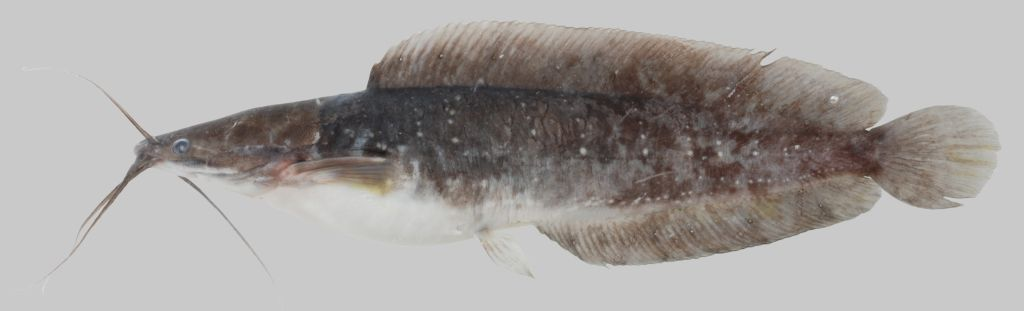
\includegraphics{images_species/152_Clarias_macrocephalus_CTU-P00116.jpg}
\caption{Photo of \emph{C.macrocephalus} by FiMSeA, on
\url{http://ffish.asia}}
\end{figure}

\textbf{First description}\\
\emph{Clarias macrocephalus}, commonly known as the bighead catfish, was
first described by \href{https://www.gbif.org/species/5202728}{Günther
in 1864}.

\#\#\#\#Scientific Research on the Species in the ASEAN Region

\textbf{Research categories}\\
Much of the research on \emph{Clarias macrocephalus} in the region is
categorised as Fisheries (20), Marine and Freshwater Biology (15), and
Biochemistry \& Molecular Biology (4).

\textbf{Research summary}\\
\emph{Clarias macrocephalus} is an economically important fish in
Thailand and is increasingly being cultivated in aquaculture
settings\citep{Na_Nakorn_2004}. However \emph{C. macrocephalus} doesn't
cultivate well and also has a near threatened status across its wild
population range because of habitat loss; as such, much of the research
effort is attempting to identify ways to increase production in
aquaculture and minimise harm to the wild population.

A genetic population study examined the success of crosses between males
of various strains of the fast growing African catfish \emph{C.
gariepinus} and females of strains of \emph{C. macrocephalus} - which
has tastier flesh - and found some hybrid strains had greater absolute
growth rate than others \citep{Koolboon_2014}. The use of hybrids has
led to some conservation concerns in Thailand regarding the wild
population of \emph{C. macrocephalus} becoming back crossed with
artificially created hybrids that have escaped from cultured systems. A
study in Thailand took DNA samples from 25 natural populations of
\emph{C. macrocephalus} from across the country - they found 12 of the
populations contained alleles in them from the African \emph{C.
gariepinus} \citep{Na_Nakorn_2004}. The hybrid is able to breed with
both species which could lead to species extinction and also grows
faster than \emph{C. macrocephalus} and so might out-compete the native
stock for resources \citep{Na_Nakorn_2004}.

Hara, M. et al., 1998, examined genetic distance in 4 wild populations
in Thailand, they found two population groups, which were
Chiangrai-Prachinburi and Pattani-Yala group and genetic distance was
larger within the first group than those within the second group.

Much of the research literature is focused on maximising yield in
aquaculture settings through studying immunity to pathogens, as well as
factors affecting growth and reproduction. Bacterial infection by
\emph{Aeromonas hydrophila} increased expression of the gene `HSC70-2'
in the tissues of \emph{C. macrocephalus} which may relate to the role
of HSC70-2 in the immune response of the species \citep{Poompoung_2012}.
\citet{Poompoung_2012} found the C3 protein produced in the liver of
\emph{C. macrocephalus} had an essential role in immunity -- furthermore
an increase in C3 was induced by beta glucan in the diet of the fish.

The effect of stocking densities in aquacultures was investigated and
found to be density dependent - \emph{C. macrocephalus} fry reared at
285 m(-3) in tanks and at 114 m(-3) in ponds had significantly faster
growth rates than fish reared at higher densities \citep{Bombeo_2002}.
Myostatin levels were found to have a negative feedback effect, rising
levels reducing growth rate in larvae of \emph{C. macrocephalus} when
they were fasted for a period of time \citep{Kanjanaworakul_2014}.

Methods of increasing reproduction, whilst minimising numbers of
broodstock were investigated in the literature - as numbers of \emph{C.
macrocephalus} are limited. One study examined 5 forms of Gonadotropin
releasing hormones to see the efficacy at stimulating ovulation in
\emph{C. macrocephalus}. Chicken GnRH was most effective as identical to
catfish Gn RH \citep{Ngamvongchon_1992}. Another study looked at the
success of using irradiated sperm of another fish species for
gynogenesis - creating offspring with only the mothers DNA
\citep{Na_Nakorn_2004}. Another study examined the properties required
to create artificial seminal plasma to be able to dilute \emph{C.
macrocephalus} milt whilst still giving high fertilisation success of
eggs -so less males are sacrificed during artificial insemination
\citep{Tan_Fermin_1999}. \emph{Clarias macrocephalus}, harvested from
irrigated rice fields in Malaysia, showed that spawning changes with
water level \citep{Ali_1993}.

What to feed \emph{Clarias macrocephalus} in culture was investigated by
Bolivar and Fermin 1996, who found that catfish larvae can be given a
dry diet, but growth rate is higher if live feed - artemia - is given
prior to the dry formula diet \citep{Fermin_1996}.

\textbf{Aquatic or marine?}\\
In a sector review of aquaculture in Thailand by the FAO \emph{Clarias
macrocephalus} and its hybrid with \emph{C. gariepinus} are listed as
freshwater species, not listed within the commercial brackish water
production section of the report. There has been some discussion of the
possibility of introducing some catfish species into brackish water
aquaculture to make use of available coastal locations, but we didn't
find any reference to this having occurred for this species.\footnote{Source:
  \url{https://www.researchgate.net/profile/Douglas_Clay/publication/313167412_Preliminary_observations_on_salinity_tolerance_of_Clarias_lazera_from_Israel/links/58d73761aca2727e5ee94ab6/Preliminary-observations-on-salinity-tolerance-of-Clarias-lazera-from-Israel.pdf}}

\textbf{Is there a description of any research locations that you can
identify?}

A conservation biology study in Thailand by \citet{Na_Nakorn_2004} took
DNA samples from 25 natural populations of \emph{C. macrocephalus} from
across the country including- 12 populations from provinces located in
the Chaophraya river basin in the centre of the country, 5 from the
Mekong river basin, 1 from the east and 7 from the south of Thailand -
they found 12 of the populations contained alleles in them from the
African \emph{C. gariepinus} \citep{Na_Nakorn_2004}. Another genetic
study in Thailand OF \emph{C. macrocephalus}, by Hara, M. et al in 1998,
assayed 14 proteins across 4 wild populations from the north
(Chiangrai), central (Prachinburi) and south (Pattani and Yala) of
Thailand.

In 1987, \emph{C. macrocephalus} were sampled monthly from the rice
fields, sump ponds and irrigation canals of North Kerian area up to
about the latitude 5°45', Northwestern Peninsular Malaysia the fish are
considered as one population \citep{Ali_1993}.

\hypertarget{patent-activity}{%
\subsection{Patent activity}\label{patent-activity}}

There are only 2 patent documents for \emph{C. macrocephalus}. The most
commonly cited patent document being for
\href{https://www.lens.org/lens/patent/WO_2008_084074_A2}{a specialized
feed for sensitive organisms, especially larvae or juvenile forms of
farmed aquatic organisms and the method of producing the feed.}.

The other \emph{C. macrocephalus} patent document is for
\href{https://www.lens.org/lens/patent/WO_2009_063044_A1}{the use of
vitamin K3 for treatment of parasitic disease in an individual, such as
an animal or human being. Vitamin K3 has been found to be effective in
the treatment of fish suffering from parasite infestation}.

A public patent collection is available for this species from
\href{https://www.lens.org/lens/collection/24937}{the Lens}.

\hypertarget{lates-calcarifer}{%
\section{\texorpdfstring{\emph{Lates
calcarifer}}{Lates calcarifer}}\label{lates-calcarifer}}

\textbf{Species name:} \emph{Lates calcarifer} \textbf{Kingdom:}
Animalia \textbf{Phylum:} Chordata
\href{https://www.gbif.org/species/2223871}{GBIF}

\textbf{Brief Description of the Species:}

The Barramundi or Asian seabass (\emph{Lates calcarifer}) is a widely
distributed species of salt and freshwater sportfish, with large, silver
scales, which can change shade, depending on their environments.
\emph{L. calcarifer} bodies can reach up to 1.8 m (6 ft) long, and the
maximum weight is about 60 kg (130 lb). The average length is about
0.6-1.2 m (2--4 ft). It is very popular in Thai cuisine.\footnote{\url{http://eol.org/pages/204766/overview}}

\emph{Lates calcarifer} are demersal, inhabiting coastal waters,
estuaries, lagoons, and rivers; they are found in clear to turbid water,
usually within a temperature range of 26−30 °C. This species does not
undertake extensive migrations within or between river systems, which
has presumably influenced establishment of genetically distinct stocks
in Northern Australia.

\begin{figure}
\centering
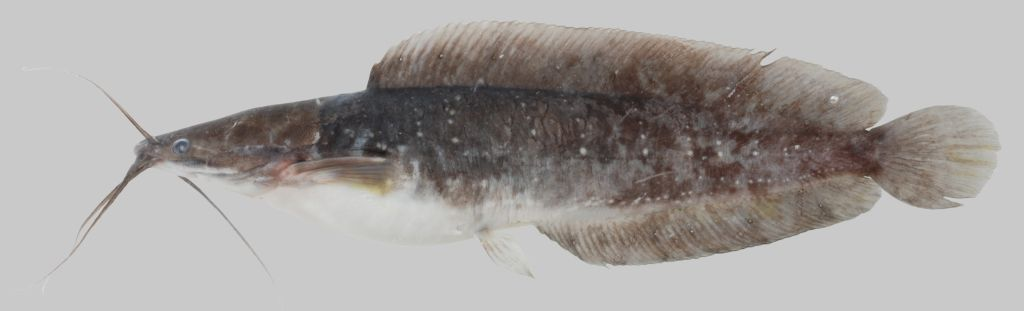
\includegraphics{images_species/152_Clarias_macrocephalus_CTU-P00116.jpg}
\caption{By Mitch Ames, Licensed under Creative Commons Attribution}
\end{figure}

\textbf{Known Distribution of the Species}\\
\emph{Lates calcarifer} are a widely distributed species - from the
Persian Gulf, through Southeast Asia to Papua New Guinea and Northern
Australia. \footnote{\url{http://eol.org/pages/204766/overview}}

\textbf{First description}\\
\emph{Lates calcarifer} was first descibed by German scientist Bloch, in
1790, and orginally named
\href{https://www.gbif.org/species/2393172}{\emph{Holocentrus
calcarifer}} .

\hypertarget{scientific-research-on-the-species}{%
\subsection{Scientific Research on the
Species}\label{scientific-research-on-the-species}}

\textbf{Research categories}\\
Much of the research on \emph{Lates calcarifer} is categorised as
Fisheries (53), Marine and Freshwater Biology (45), Veterinary Sciences
(13), Biotechnology \& Applied Microbiology (9), Genetics \& Heredity
(8).

\textbf{Research summary}\\
Much of the research effort regarding \emph{L. calcarifer} is concerned
with optimising conditions for successful aquaculture of this valuable
fish species. Some studies have investigated the natural history of the
fish, particularly spawning and juveniles, as was the case in a study
using controlled incubation of wildstock from the inland waters of
Vietnam \citep{Shadrin_2015}.

Others have focused on optimising feed for this species -- noting the
success of live food in a study in the South China Sea
\citep{Shansudin_1997}. Others noted physiological aspects of nutrition
-- essential fatty acid metabolism in \emph{L. calcarifer}
\citep{Mohd_Yusof_2010}. Some studies have trialled the use of local
seaweed species - K. alvarezii, E. denticulatum and S. polycystum -- to
replace commercial feed binder in the feed of \emph{L.calcarifer}
juveniles \citep{Shapawi_2015}.

The genetics of \emph{Lates calcarifer} have been the subject of some
investigation by scientists with one study looking at the chromosomes of
male and female fish \citep{Phimphan_2015}. Prevalent diseases which
effect successful aquaculture were also given attention in the
literature with one study noting the pathological effects of SDS in
\emph{L.calcarifer} indicating it to be a viral infection
\citep{Gibson_Kueh_2011}.

Fish aquaculture has an effect on the environment; this was the subject
of a study examining pelagic carbon flow and water chemistry in mangrove
estuaries with fish cage aquaculture of \emph{L.calcarifer}
\citep{Alongi_2003}.

\textbf{Aquatic or marine?} \emph{Lates calcarifer} live close to the
sea floor, inhabiting coastal waters, estuaries, lagoons, and rivers;
they are found in clear to turbid water - within a temperature range of
26−30 °C. \footnote{\url{http://eol.org/pages/204766/overview}}

This species is able to adapt to a range of salinities and thus are
found in freshwater, estuarine, lagoons, brackish, rivers and coastal
areas \citep{Davis_1986}. It has been shown that some of the fish move
between salt and freshwater environments whilst others remain only in
the marine environment \citep{Davis_1986}.

Adults in freshwater usually migrate to spawn in water with higher
salinity as eggs need saltwater to develop. Spawning most often occurs
in brackish water like the river mouth and is seasonal
\citep{Moore_1982}.

\textbf{Research locations}

Marine fisheries in the Gulf of Thailand were the subject of a study
looking at changes in 35 marine species including \emph{Lates
calcarifer} over a 26 year period \citep{Tuantong_2015}.

Mangrove inlets and creeks in Selangor, Malaysia are the habitat for 119
species of fish (the majority of which are juveniles)- the common fish
species included \emph{Lates calcarifer} \citep{Sasekumar_1992}. The
tidally dominated mangrove estuaries of peninsualr Malaysia were the
location of a study examining the environmental effects of fish cage
aquaculture of \emph{L.calcarifer} \citep{Alongi_2003}.

\hypertarget{patent-activity-1}{%
\subsection{Patent activity}\label{patent-activity-1}}

The majority of patent activity centres around aquaculture,
specifically, \href{WO\%202008/084074\%20A2}{feed},
\href{WO\%202010/027788\%20A1}{products} and
\href{WO\%202009/063044\%20A1}{methods}.

\href{US\%202012/0114570\%20A1}{Patent activity includes the novel use
of fish skin including lates calcarifer as an industrial source of
collagen}, (US 2012/0114570 A1).

\href{WO\%202014/094918\%20A1}{Medical and cosmetic skin treatments have
also been derived from the hatching fluid of fish including lates
calcarifer}.

\href{https://www.lens.org/lens/collection/25319}{A patent collection is
available for this species from the Lens}

\hypertarget{litopenaeus-vannamei}{%
\section{\texorpdfstring{\emph{Litopenaeus
vannamei}}{Litopenaeus vannamei}}\label{litopenaeus-vannamei}}

\begin{itemize}
\tightlist
\item
  \textbf{Species name:} \emph{Litopenaeus vannamei}
\item
  \textbf{Kingdom:} Animalia
\item
  \textbf{Phylum:} Arthropoda
  \href{https://www.gbif.org/species/2223871}{GBIF}
\end{itemize}

\textbf{Brief Description of the Species:}\\
The dominant shrimp culture species in the world, they are benthic -
occurring in waters of depth between 0-72m in marine habitats as adults,
and estuarine environments as juveniles in subtropical to tropical
climates.\^{}{[}Source:
\url{http://www.sealifebase.org/summary/Litopenaeus-vannamei.html}. Asia
has seen a phenomenal increase in the production of \emph{L. vannamei},
no production was reported to FAO in 1999, but by 2004 it was nearly 1
116 000 tonnes having overtaken the production of \emph{P. monodon} in
China, Taiwan Province of China and Thailand. However, due to fears of
importing exotic diseases it is only experimentally farmed in Cambodia,
India, Malaysia, Myanmar and the Philippines. Thailand and Indonesia
both freely permit its commercial culture but have official
restrictions, so that only SPF/SPR broodstock may be imported.\footnote{Source:
  \href{http://www.fao.org/fishery/culturedspecies/Penaeus_vannamei/en}{FAO
  at http://www.fao.org/fishery/culturedspecies/Penaeus\_vannamei/en}}

\begin{figure}
\centering
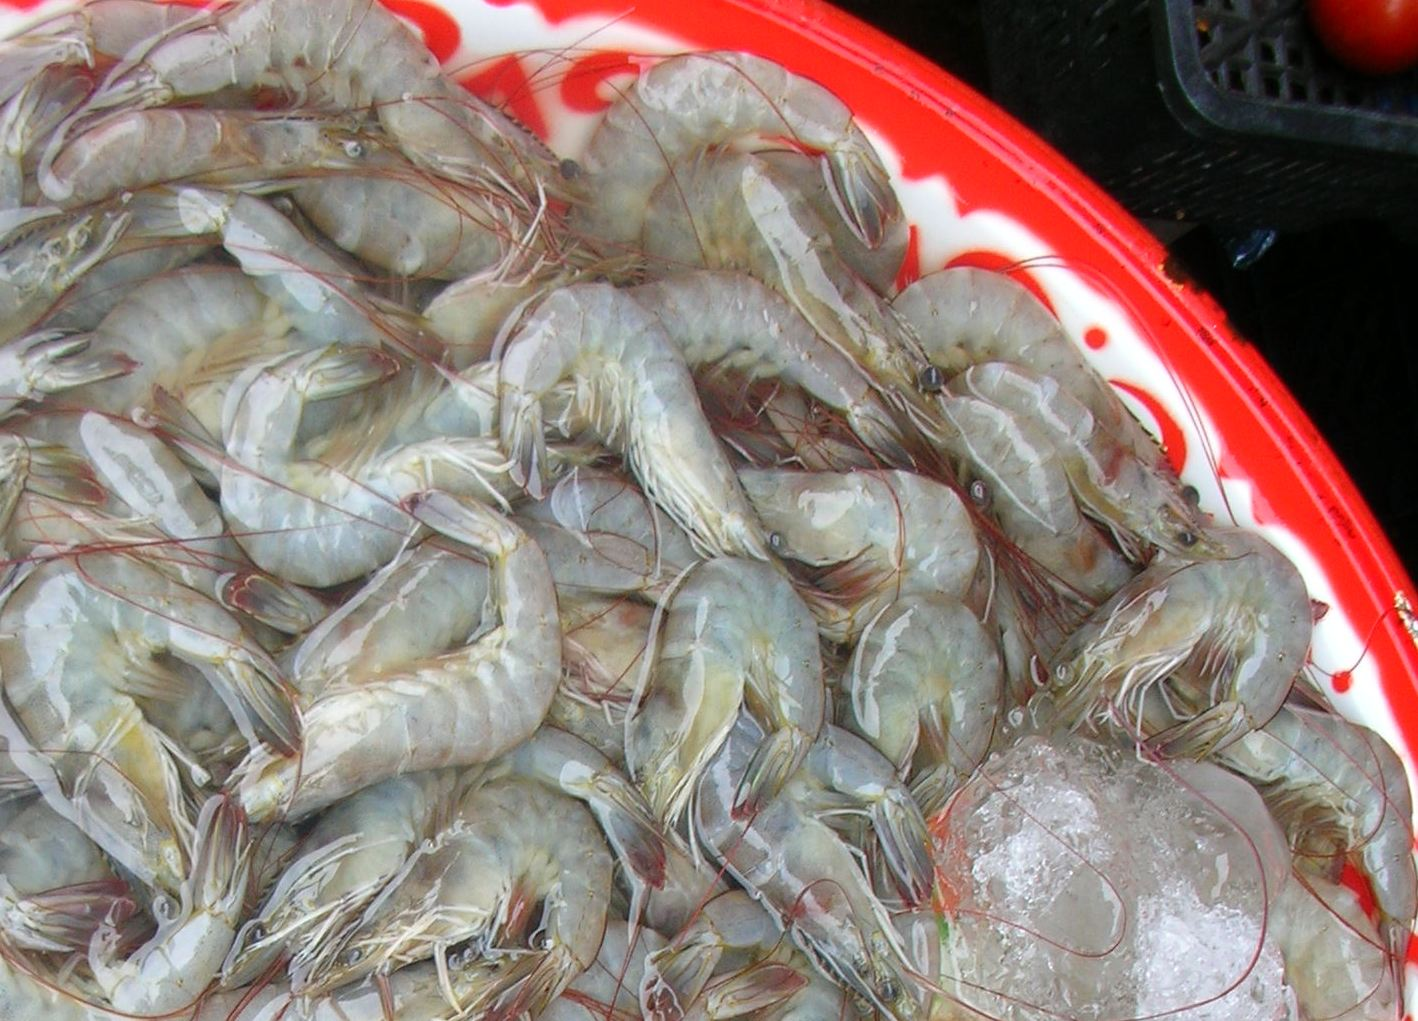
\includegraphics{images_species/Litopenaeus_vannamei55.jpg}
\caption{By Xufanc (Own work)}
\end{figure}

\textbf{Known Distribution of the Species}\\
\emph{Litopenaeus vannamei} is native to the Eastern Pacific coast from
Sonora, Mexico in the North, through Central and South America as far
South as Tumbes in Peru.\^{}{[}Source:
\href{http://www.fao.org/fishery/culturedspecies/Penaeus_vannamei/en}{FAO
at http://www.fao.org/fishery/culturedspecies/Penaeus\_vannamei/en} .

The main producer countries of Penaeus vannamei are: China, Thailand,
Indonesia, Brazil, Ecuador, Mexico, Venezuela, Honduras, Guatemala,
Nicaragua, Belize, Viet Nam, Malaysia, Tawian P.C., Pacific Islands,
Peru, Colombia, Costa Rica, Panama, El Salvador, the United States of
America, India, Philippines, Cambodia, Suriname, Saint Kitts, Jamaica,
Cuba, Dominican Republic, Bahamas.\footnote{Source: {[}FAO at
  \url{http://www.fao.org/fishery/culturedspecies/Penaeus_vannamei/en}{]}
  (\url{http://www.fao.org/fishery/culturedspecies/Penaeus_vannamei/en})}

\textbf{First description}\\
\emph{Litopenaeus vannamei} was first described in 1931 as \emph{Penaeus
vannamei} by Boone.\footnote{Source:
  \href{https://www.gbif.org/species/2223871}{GBIF at
  https://www.gbif.org/species/2223871}}

\hypertarget{scientific-research-on-the-species-in-the-asean-region}{%
\subsection{Scientific Research on the Species in the ASEAN
Region}\label{scientific-research-on-the-species-in-the-asean-region}}

\textbf{Research categories}\\
Much of the research on \emph{Litopenaeus vannamei} is categorised as
Fisheries (54), Marine and Freshwater Biology (32), Veterinary Sciences
(26), Biotechnology \& Applied Microbiology (10), Immunology (10),
Biochemistry and Molecular Biology (6).

\textbf{Research summary}\\
Much of the research on \emph{Litopenaeus vannamei} as the worlds
dominant cultured shrimp species was with regard to maximising yield,
through selecting robust broodstock as well as via disease treatment and
prevention.

Researchers found that cold storage of spermatophores from broodstock
was effective by combining an antibiotic within the mineral oil
surrounding the sperm \citep{Tuantong_2015}. Another study focussed on
reproduction of \emph{Litopenaeus vannamei} looked at the success of
crosses with limited numbers of males and females, and noted that male
broodstock could be selected with desirable traits
\citep{Aungsuchawan_2008}.

Diseases of \emph{Litopenaeus vannamei} and other commercially farmed
shrimps blight production and so much of the research literature is
focussed on how to overcome some of these diseases: via longer rearing
and less dense stocking to protect against infectious myonecrosis
(10.1016/j.jip.2010.03.001), or introduction of immune stimulating
agents PAP-phMGFP (10.1016/j.fsi.2011.06.010)and CHH
(10.1016/j.fsi.2011.01.014). Another study found the use of dsRNA
injected into prawns to be effective as both a preventative, and
treatment for Penaeus stylirostris densovirus (PstDNV)
infection(10.1016/j.virusres.2010.09.009). Similarly galangal extract
and trans-p-coumaryl diacetate stimulated the immune system response,
thereby promoting resistance to V. harveyi infection in
\emph{Litopenaeus vannamei}(10.1007/s10499-014-9822-2). Detecting Taura
Syndrome Virus in Shrimps via diagnostic test kits was the subject of
another study (10.3354/dao069249)

Antibiotic resistance is a growing problem worldwide in the aquaculture
industry and for human health. As such much of the literature was
focussed on looking at alternatives to antibiotic use, such as
probiotics. One study found the use of bacteria, yeasts, and algae in
water additives or artemia enriched enhanced survival and growth rate of
\emph{Litopenaeus vannamei} (10.1016/j.anifeedsci.2011.07.003). The
probiotic Bacillus subtilis BS11 supplement was found to benefit
\emph{Litopenaeus vannamei} growth and survival after infection with
Vibrio harveyi, conferring disease resistance (10.1111/anu.12040).

The food safety of cultured seafood is paid some attention amongst the
research literature, -minimal sequential ozone treatment and ice storage
for \emph{Litopenaeus vannamei} has been shown to have an antioxidant
like action and could promise further safety for shrimp consumption
(10.1016/j.lwt.2014.02.007).

Astaxanthin extract from \emph{Litopenaeus vannamei} has been
demonstrated in one study to act as anti-inflammatory alternative
against carrageenan-induced paw oedema and pain behaviour in mice
(10.3390/molecules21030382).

Genetics were the subject of several studies in the literature including
the correlation between genetics and body weight in \emph{Litopenaeus
vannamei} (10.1111/j.1365-2052.2005.01274.x). Genetic variation and
population structure of wild \emph{Litopenaeus vannamei} from 4
geographic locations from Mexico to Panama were investigated using 5
microsatellite DNA and it was found that subpopulations exist
(10.1007/s10126-004-3138-6).

\textbf{Aquatic or marine?} \emph{Litopenaeus vannamei} live in marine
habitats as adults, and estuarine environments (brackish water) as
juveniles in subtropical to tropical
climates(\url{http://www.sealifebase.org/summary/Litopenaeus-vannamei.html}

\textbf{Is there a description of any research locations that you can
identify?}\\
Brazil and Indonesia are mentioned in a study on infectious myonecrosis
of Brazilian farmed \emph{Litopenaeus vannamei}
(10.1016/j.jip.2010.03.001).

China, Thailand, Peru to Mexico on the Pacific coast, and Taiwan are
referenced in a paper about the most widely cultured alien crustacean in
the world \emph{Litopenaeus vannamei} (10.1007/978-94-007-0591-3\_17).
Genetic variation among 4 populations of \emph{L.vannamei} from
locations along the coast between Mexico and Panama were the subject of
one investigation which noted subpopulations were present
(10.1007/s10126-004-3138-6).

\emph{Enterocytozoon hepatopenaei} has been found in \emph{L.vannamei}
farms across India - within the states of: Tamil nadu, Andhra Pradesh
and Odisha. \emph{E.hepatopenaei} has also been detected in shrimp
cultured in China, Vietnam and Thailand and is suspected to have
occurred in Malaysia and Indonesia and to be linked with severely
retarded growth (10.3354/dao03036).

\hypertarget{patent-activity-2}{%
\subsection{Patent activity}\label{patent-activity-2}}

There are 309 patent documents for \emph{Litopenaeus vannamei}, the most
commonly cited
\href{https://www.lens.org/lens/patent/US_6615767_B1}{patent being for a
commercial aquaculture system using algae and artemia as food stuffs for
juveniles}. Many other patent documents relate to differing forms of
aquaculture system for growing \emph{Litopenaeus vannamei}. Other
\emph{L. vannamei} patent documents relate to
\href{https://www.lens.org/lens/patent/CN_102648738_A}{feed
compositions, such as one without fish meal}.

Some patent documents for \emph{L. vannamei} relate to inducing immune
responses, for example
\href{https://www.lens.org/lens/patent/US_2005_0080032_A1}{using dsRNA
to modulate gene expression and responses to pathogens}.

\href{https://www.lens.org/lens/collection/24984}{Lens collection}

\hypertarget{macrobachium-rosenbergii}{%
\section{\texorpdfstring{\emph{Macrobachium
rosenbergii}}{Macrobachium rosenbergii}}\label{macrobachium-rosenbergii}}

\begin{itemize}
\tightlist
\item
  \textbf{Species name:} \emph{Macrobachium rosenbergii}\\
\item
  \textbf{Kingdom:} Animalia\\
\item
  \textbf{Phylum:} Arthropoda
  \href{https://www.gbif.org/species/2224546}{GBIF}
\end{itemize}

\textbf{Brief Description of the Species:}\\
\emph{Macrobachium rosenbergii} known as the Giant River Prawn and the
Giant Freshwater Prawn - it is widely fished and also is the main
freshwater shrimp cultivated within the commercial aquaculture industry,
\href{http://www.iucnredlist.org/details/197873/0}{IUCN}. The body
length of this large prawn species is 320 mm for males; and 250 mm for
females, as it is a sexually dimporphic species.
\href{http://www.fao.org/fishery/culturedspecies/Macrobrachium_rosenbergii/en}{FAO.org}.

Global production of the Giant River Prawn has grown since its inception
in the 1970's and by 2002 was 200 000 tonnes/yr
\href{http://www.fao.org/fishery/culturedspecies/Macrobrachium_rosenbergii/en}{FAO.org}.

\textbf{Known Distribution of the Species}\\
\emph{M. rosenbergii} is native to Bangladesh; Brunei Darussalam;
Cambodia; China; India; Indonesia (Java); Malaysia (Peninsular Malaysia,
Sabah, Sarawak); Myanmar (Myanmar (mainland)); Pakistan; Philippines;
Singapore; Sri Lanka; Thailand
\href{http://www.iucnredlist.org/details/197873/0}{IUCN}. The geographic
distribution is now much wider than this as it has been introduced to
all continents for aquaculture and is now found in Brazil, Venezuela,
Australia, United States, Iceland, Japan, Germany, Iran,
Taiwan,\href{https://www.gbif.org/species/2224546}{GBIF}.

\textbf{First description}\\
\emph{M. rosenbergii} was first described by Johannes De Man in 1879 as
\emph{Palaemon rosenbergii} in the publication: De Man, 1879, Notes
Leyden Mus., 1:167, however in 1966 Johnson renamed it to its current
nomenclature of \emph{Macrobachium rosenbergii}
\href{http://www.fao.org/fi/oldsite/eims_search/advanced_s_result.asp?JOB_NO=AC477}{(Holthuis,L.B.
1980)}.

\begin{figure}
\centering
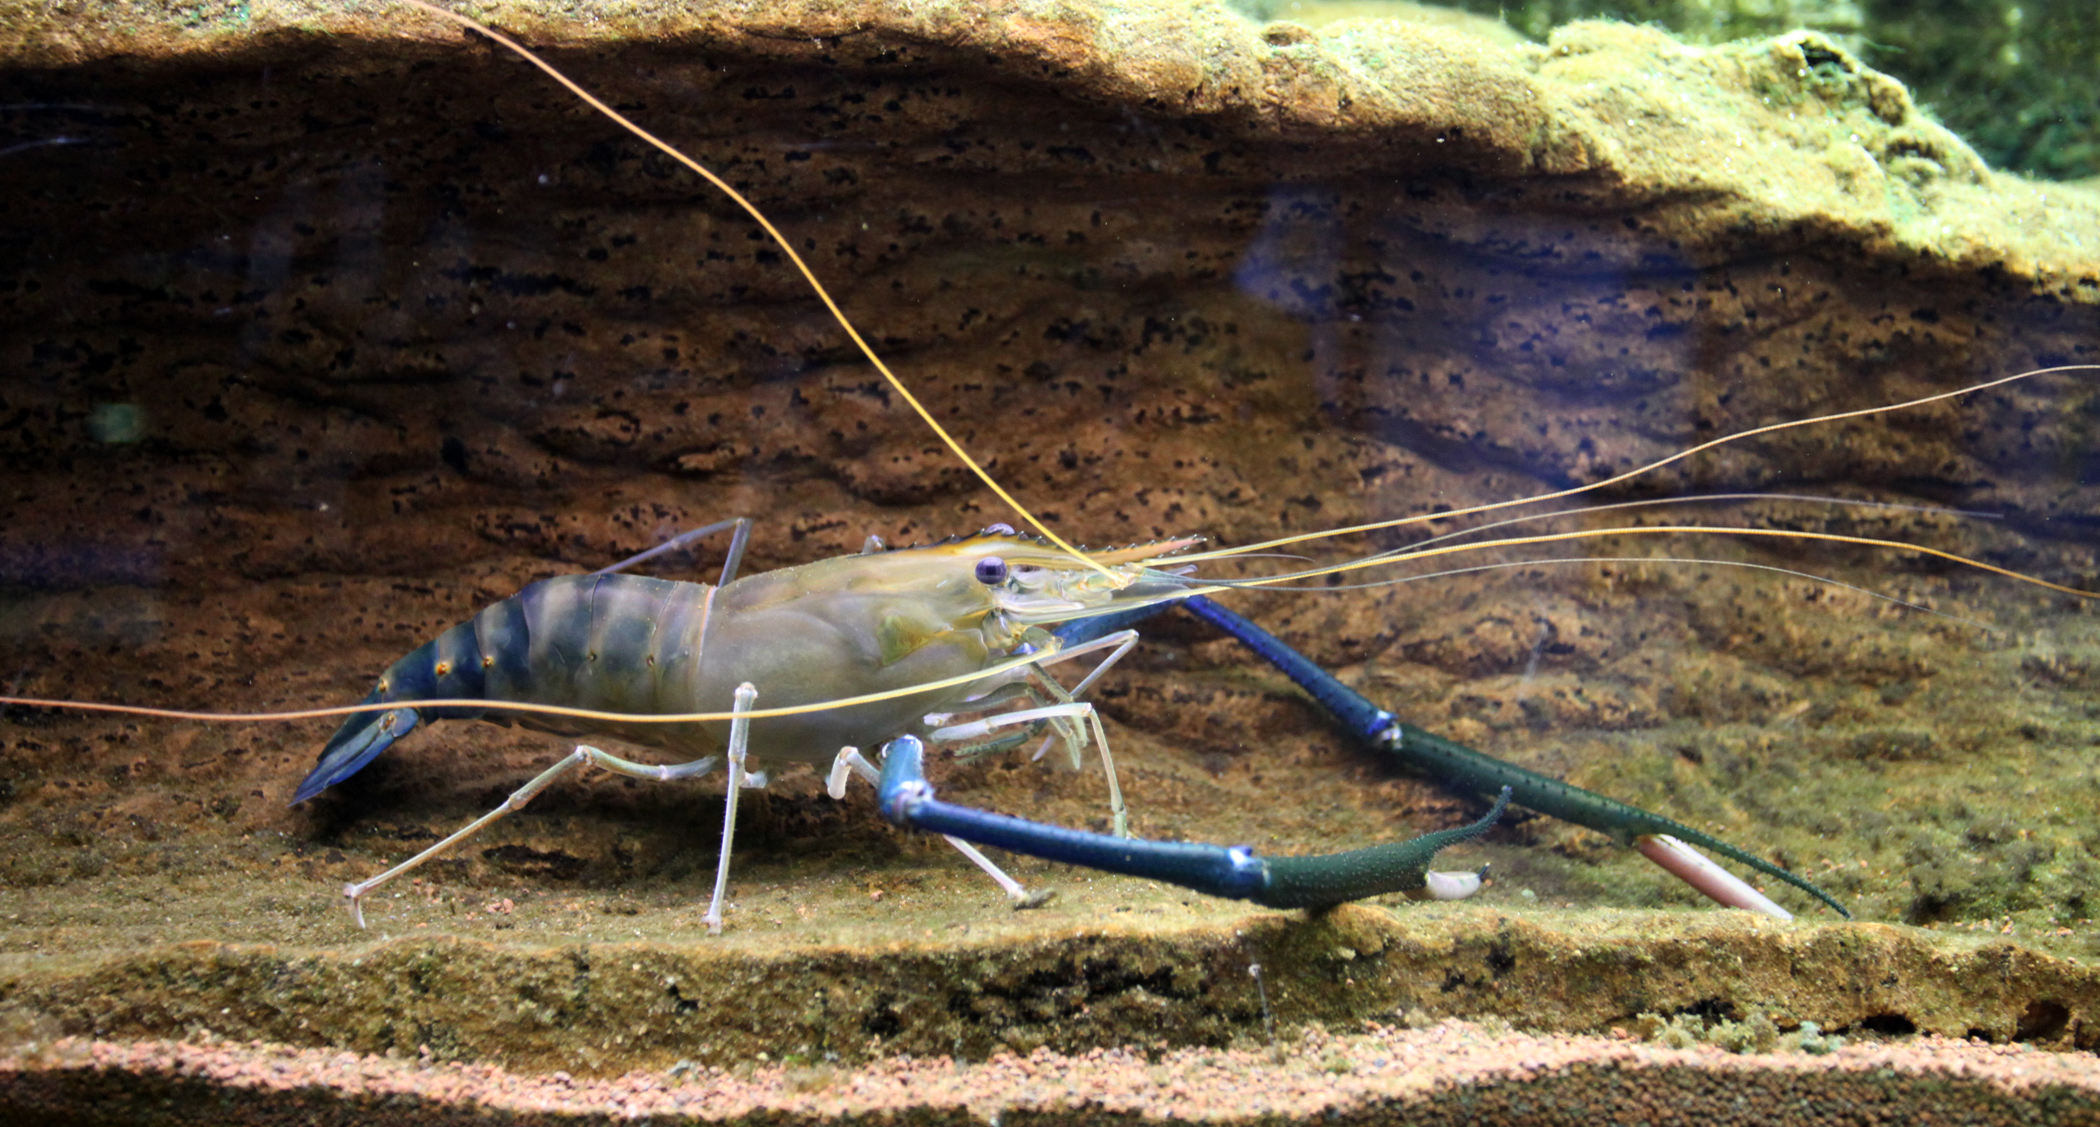
\includegraphics{images_species/Macrobrachium_rosenbergii.jpg}
\caption{© Citron / CC BY-SA 3.0}
\end{figure}

\hypertarget{scientific-research-on-the-species-in-the-asean-region-1}{%
\subsection{Scientific Research on the Species in the ASEAN
Region}\label{scientific-research-on-the-species-in-the-asean-region-1}}

\textbf{Research categories}\\
Much of the research on \emph{M. Rosenbergii} in the region is
categorised as fisheries (77), followed by Marine and Freshwater Biology
(46), Biochemistry \& Molecular Biology (21), Veterinary Sciences (20),
Zoology (13), Immunology (12) amongst others.

\textbf{Research summary}\\
The majority of the research effort on \emph{Macrobachium rosenbergii}
is directed towards maximising aquaculture yield to increase economic
gain of shrimp farmers. So the research is broadly concerned with
disease prevention/treatment, nutrition, stocking densities,
reproductive success, and genetic make up of broodstock. Understanding
the diseases of \emph{M.rosenbergii} - such as \emph{L. garvieae} a
bacteria that infects shrimps (Dangwetngam, M. and Suanyuk, N. 2014),
and White Tail Disease virus (10.1016/j.jip.2010.09.007) which causes
large scale mortality in aquaculture populations- can enable treatments
and preventative strategies to be adopted. Improving yield of shrimp
farmers has led many to look to the genetic quality of broodstock -
analysing the parentage of existing broodstock
(10.1016/j.aquaculture.2011.10.045), as well as comparing this with wild
samples (10.1016/j.bse.2014.12.023).This genetic analysis can then help
develop a more successful breeding strategy
(10.1016/j.aquaculture.2009.12.011). The nutritional composition of feed
given to farmed \emph{M.rosenbergii} is another common theme of research
in the literature, as well fed shrimps grow bigger and reproduction is
increased (10.7717/peerj.2735). However for shrimp farmers in the Mekong
Delta region of Vietnam, identifying non commercial feed options - due
to affordability issues- is key (10.1111/j.1444-2906.2005.00961.x).
Understanding how eye stalks inhibit reproduction in female
\emph{M.rosenbergii} (10.2306/scienceasia1513-1874.2014.40.157), as well
as understanding how sex differentiation occurs (10.3390/ijms17050690)
and when to intervene to create all male stock
(10.1016/j.aquaculture.2012.03.015) are some of the reproductive
focussed areas of research covered in the literature.

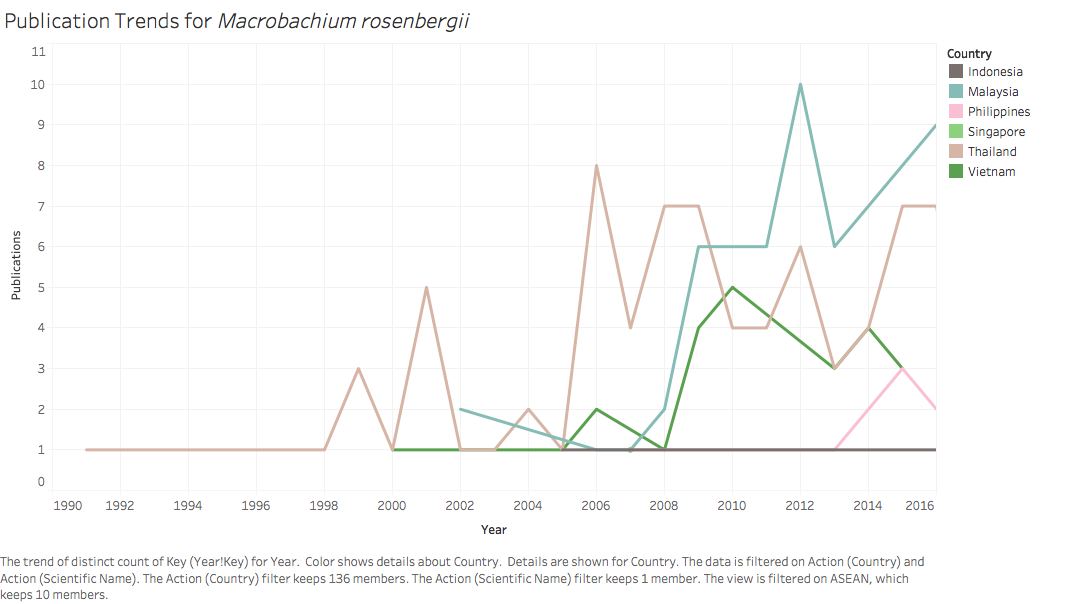
\includegraphics{images_species/Publication trend for Macrobachium rosenbergii.png}

\textbf{Aquatic or marine?} Although \emph{M. rosenbergii} is
predominantly a tropical freshwater species, the larval stage of the
species is found within adjacent brackish water, as females migrate to
estuaries to lay their eggs
\href{http://www.fao.org/fishery/culturedspecies/Macrobrachium_rosenbergii/en}{FAO.org}.Most
of the \emph{M. rosenbergii} farms are in freshwater inland locations,
however some are in estuarine and coastal locations where salinity in
the ponds can fluctuate and effect breeding success of females
(10.1016/j.aquaculture.2008.04.035).

\textbf{Is there a description of any research locations that you can
identify?}\\
Much of the research involves laboratory bred cultures of
\emph{M.rosenbergii}, although some studies do include wild samples as
is the case in a genetic study by Schneider et al 2013
910.1111/j.1365-2109.2012.03147.x). Schneiders' study used cultured
prawn samples from: Andhra Pradesh, India; Kaneohe, Hawaii, USA;
Tamashiro Market, Honolulu, Hawaii, USA; University of Negev, Beer
Sheva, Israel;Frankfort, Kentucky, USA; Leland, Mississippi, USA;
Weatherford, Texas, USA as well as wild prawn samples from Hmaw River,
Hlaing River and the Pan Hlaing River - tributaries of the Yangon River,
Yangon, Myanmar; and Mahanadi River, Orissa, India. There are some
references to more specific locations for wild samples within the
literature - such as research into a breeding strategy for genetic
improvement using wild strains Vietnam (Dong Nai and Mekong)
(10.1016/j.aquaculture.2009.12.011)(10.1111/jwas.12148).\emph{L.
garvieae} was isolated from \emph{M.rosenbergii} samples taken from
cultures and wild prawns from the Phatthalung and Songkhla, provinces of
southern Thailand (Dangwetngam, M. and Suanyuk, N., 2014). Some research
doesn't specify anything more than the country such as in a study
detailing culture technology in Thailand
(10.1111/j.1365-2109.2011.03037.x). Genetic diversity analysis was
undertaken on cultured samples from farms in Zhejiang, Guangdong and
Guangxi provinces, China, as well as wild samples from Dong Nai River
and Mekong River, Vietnam (10.1016/j.bse.2014.12.023).

\hypertarget{patent-activity-3}{%
\subsection{Patent activity}\label{patent-activity-3}}

The top cited patent involving \emph{M.Rosenbergii} is regarding
\href{https://www.lens.org/lens/patent/WO_2008_084074_A2}{feed
composition for shrimps in aquaculture settings}. The invention
specifies a range of percentage compositions of
lipid:carbohydrate:protein, differing nutritional sources, particle size
and types - as an alternative to live feed for shrimp larvae.

The largest family number of a patent associated with
\emph{M.Rosenbergii} is for another type of feed, this time for
{[}preparation and use of methionylmethionine as a feed additive for
fish And crustaceans{]}
(\url{https://www.lens.org/lens/patent/US_2010_0098801_A1}).

\href{https://www.lens.org/lens/collection/24802}{Lens collection}

\hypertarget{nypa-fruticans}{%
\section{\texorpdfstring{\emph{Nypa
fruticans}}{Nypa fruticans}}\label{nypa-fruticans}}

\begin{itemize}
\tightlist
\item
  \textbf{Species name:} \emph{Nypa fruticans}
\item
  \textbf{Kingdom:} Plantae
\item
  \textbf{Phylum:} Tracheophyta
  \href{https://www.gbif.org/species/2738422}{GBIF}
\end{itemize}

\textbf{Brief Description of the Species:}\\
\emph{Nypa fruticans} is a palm found in the upstream estuarine zone in
all intertidal regions. It forms extensive belts along brackish to tidal
freshwater creeks and rivers. It is very fast growing, especially in
fresh water, and is a competitive species
(\url{http://eol.org/pages/1137487/details}). It is the only palm
adapted to the mangrove biome and grows in terrestrial, marine and
freshwater habitats.

The trunk of \emph{Nypa fruticans} grows underground with the leaves,
female flower inflorences and male flowers visible above the ground
(\url{http://www.efloras.org/florataxon.aspx?flora_id=2\&taxon_id=220009317}).

\emph{Nypa fruticans} is used for a wide range of commercial goods and
services including- thatching and for making alcoholic drinks through a
fermentation process(\url{http://www.iucnredlist.org/details/178800/0}).
It is an important emerging source of biofuel, capable of producing
ethanol ranging from 6,480 to 20,000 L/ha, a higher yield than
sugarcane(\url{http://agris.fao.org/agris-search/search.do?recordID=MY2015000742}).
It is considered to be of 'Least concern as it is widespread and locally
common (\url{http://www.iucnredlist.org/details/178800/0}).

\begin{figure}
\centering
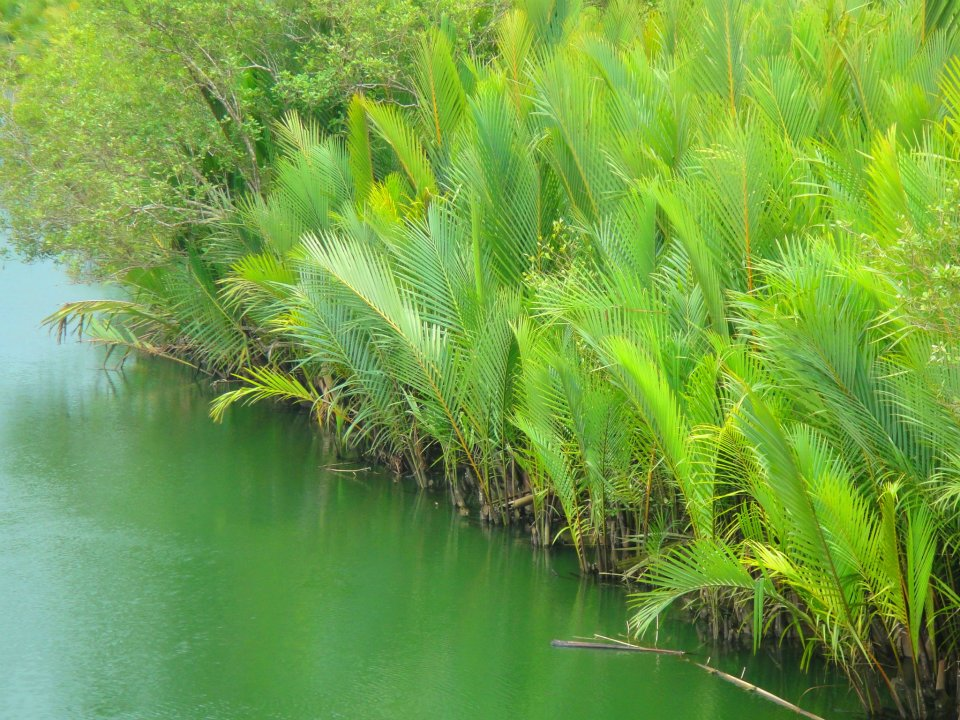
\includegraphics{images_species/Nipa_palms.jpg}
\caption{By Qaalvin Own work}
\end{figure}

\textbf{Known Distribution of the Species}\\
\emph{Nypa fruticans} ranges from Sri Lanka and the Ganges Delta through
to the west Pacific. In South and South-East Asia it is found in
Bangladesh, Brunei Darussalam, Cambodia, China, India, Indonesia, Japan,
Malaysia, Myanmar, Singapore, Sri Lanka, Thailand, and Viet Nam . In
much of its native range it has been planted and exists in large or
small-scale plantations (\url{http://eol.org/pages/1137487/overview}).

\emph{Nypa fruticans} has been introduced to Cameroon and Nigeria in
West Africa and to Panama in Central America and Trinidad and Tobago in
the Caribbean. (\url{http://eol.org/pages/1137487/overview}).

\textbf{First description}\\
\href{https://www.gbif.org/species/2738422}{\emph{Nypa fruticans} was
first described by a German botanist called Christoph Carl Friedrich von
Wurmb in 1781}.

\hypertarget{scientific-research-on-the-species-1}{%
\subsection{Scientific Research on the
Species}\label{scientific-research-on-the-species-1}}

\textbf{Research categories}\\
Much of the research on \emph{Nypa fruticans} is categorised as
Environmental Sciences (8), Biology (6), Marine and Freshwater Biology
(6), and Plant Sciences (6).

\textbf{Research summary}\\
Much of the research on \emph{Nypa fruticans} is studying its role
within mangrove biomes, an important ecological and economic habitat
type. In the Segara Anakan lagoon, Java, mangrove tree density and
diversity was examined at the eastern part of the lake - \emph{Nypa
fruticans} was present and characterised a mature undisturbed forest
(10.1007/s10113-008-0074-4). Within Malaysia - on Carey Island - a
similar demographic study was conducted looking at the percentage of
\emph{Nypa fruticans} seedling, juvenile, adult and mature present the
population showed a majority of adults with 67.9\% (Aslezaeim, N. and
Rozainah, MZ. 2010). Also in Malaysia a study of forest structure,
diversity index and above-ground biomass was conducted on
\emph{N.fruticans} at Tok Bali mangrove forest, Kelantan (Kamaruzaman, J
et al 2007).

Low genetic diversity for \emph{N.fruticans} was found amongst six
natural populations from China, Vietnam, and Thailand across a total of
183 individuals (10.1016/j.aquabot.2009.09.003). Creating
\emph{N.fruticans} seedlings was the focus of some research due to the
economic benefits of the plant - mass clonal propagation of disease free
planting materials was successfully trialled in one study (Abad, R G et
al 2015). In another propagation study in Vietnam, a participatory
action research methodology was used to successfully establish an
\emph{N.fruticans} (and other mangrove species) nursery on unused acid
sulphate soil -normally considered unsuitable for mangrove growth
(Nguyen, T P 2016).

Species living on \emph{N.fruticans} or within the mangrove biome it
creates were the focus some of the literature with several studies
examining the fungi present on samples from different populations. One
study tested the fungi growing on \emph{N.fruticans} for heavy metal
tolerance and found that one that was able to successfully grow deposit
heavy metal pollution - meaning it could potentially be used as a type
of absorbent material (10.1007/s12601-015-0040-2). Species diversity of
marine fungi on \emph{Nypa fruticans} in Samut Songkhram Province,
Thailand were investigated, with 81 fungal taxa recorded
(10.1515/BOT.2005.049). Taxonomy of fungus found on \emph{Nypa
fruticans} in the intertidal regions in Trang and Trat provinces,
Thailand was examined in another study (10.7872/crym/v36.iss3.2015.319).
Biodiversity and ecology of higher filamentous fungi on \emph{Nypa
fruticans} along the Tutong River, Brunei were examined during 1999,
with Forty-six taxa recorded (Hyde, K.D.and Sarma, V.V. 2006).

Both mudskippers and fireflies were found to inhabit populations of
\emph{Nypa fruticans} within the literature. Mudskippers,
\emph{Periophthalmodon septemradiatus} were recorded for the first time
in Peninsular Malaysia, from the small tributaries of the rivers
Selangor and Muar (Khaironizam, MZ and Norma-Rashid, Y. 2003). Whereas
\emph{Pteroptyx} fireflies are commonly reported to congregate in large
numbers in mangroves, but researchers found they preferred vegetation
consisting mainly of \emph{S. caseolaris} and \emph{N.fruticans}
(10.1007/s11273-009-9172-4). A study of the root-associating bacteria of
\emph{N.fruticans} found in brackish-water mud in Sarawak, Malaysia,
discovered that \emph{Burkholderia vietnamiensis} to be its main
nitrogen-fixing bacterium (10.1271/bbb.100397). Another important type
of organism examined in the literature was that of the pollinators
inhabiting \emph{N.fruticans} mangroves in an Oxford University study,
within the submerged Melaleuca forests of Vietnam (Nguyen, Q. 2008).

The economic exploitation of \emph{N.fruticans} was examined by some
researchers, one Malaysian paper looked at the ripe and unripe fruit
content to see if can be used as a food source (10.1051/fruits/2013089).
Whilst another scientist examined the potential of \emph{N.fruticans} in
the Philippines for alcohol production (Rasco, E.T., 2010).

\textbf{Aquatic or marine?}\\
\emph{N.fruticans} grows in mangrove forests in upwater estuarine
locations, so it is aquatic, and terrestrial - as it is exposed at low
tide, and marine as the salt water from the ocean meets the freshwater
of the rivers (\url{http://eol.org/pages/1137487/details}).

\textbf{Is there a description of any research locations that you can
identify?}\\
A demographic study of \emph{Nypa fruticans} was undertaken on Carey
Island Malaysia (Aslezaeim, N.and Rozainah, M.Z., 2010). Forest
structure was also examined at Tok Bali mangrove forest, Kelantan,
Malaysia Kamaruzaman (Kamaruzaman, J. et al.~2007).A study looking at
tree density and diversity of mangroves in different areas of Segara
Anakan lagoon, Java, noted the presence of \emph{N.fruticans} as an
indicator of a mature forest(10.1007/s10113-008-0074-4).

In the Vam Ray area Kien Giang Province, Vietnam, a participatory
research methodology was used to establish a mangrove nursery on soil
considered previously to be unsuitable - 5 types of mangrove species
were successfully grown grown including \emph{Nypa fruticans} seedlings
(Nguyen, T.P., 2016); providing a potential source of income for local
people.

Genetic diversity of populations from six natural populations of
\emph{Nypa fruticans} from China, Vietnam, and Thailand was assessed,
and showed an extremely low level of genetic diversity
(10.1016/j.aquabot.2009.09.003).

Selangor and Muar rivers of Malaysia were discovered to contain
mudskipper populations, whilst a 2010 study of alcohol production
potential took place in Vinzons, Camarines Norte, Philippines(Rasco,
E.T., 2010). Pollinators of \emph{Nypa fruticans} were examined in the
submerged meleuca forests of South Vietnam (Nguyen, Q. 2008) and the
bacteria inhabiting the rhizomes of \emph{Nypa fruticans} in Sarawak
Malaysia were identified (10.1271/bbb.100397).

\hypertarget{patent-activity-4}{%
\subsection{Patent activity}\label{patent-activity-4}}

There are 10 patent documents for \emph{Nypa fruticans} , the most
commonly cited patent document is for a {[}tnf-alpha and nitric oxide
production inhibitor using an extract from the plant body of the palm{]}
(\url{https://www.lens.org/lens/patent/JP_2007008817_A}).

\href{https://www.lens.org/lens/collection/24939}{Lens collection}

\hypertarget{oreochromis-niloticus}{%
\section{\texorpdfstring{\emph{Oreochromis
niloticus}}{Oreochromis niloticus}}\label{oreochromis-niloticus}}

\begin{itemize}
\tightlist
\item
  \textbf{Species name:} \emph{Oreochromis niloticus}
\item
  \textbf{Kingdom:} Animalia\\
\item
  \textbf{Phylum:} Chordata
  \href{https://www.gbif.org/species/4285694}{GBIF}
\end{itemize}

\textbf{Brief Description of the Species:}\\
\href{http://eol.org/pages/356343/overview}{\emph{Oreochromis
niloticus}} is a species of Tilapia, a cichlid fish
\href{http://eol.org/pages/356343/data?toc_id=4\#1448}{native to the
nile basin in Africa and coastal rivers of Israel}, however it's an
economically important species of fish which has been introduced widely
outside of its natural range.

\emph{O. niloticus} adults grow to 60cm and live up to 9 years weighing
up to 4.3kg. It lives in freshwater and can tolerate brackish water, wit
a temperature range of 8-42°C.It's an omnivore feeding on plankton as
well as mosquito larvae.Groups of cichlids establish social hierarchies
in which dominant males have priority for access to mate and food.

Commercial aquaculture of \emph{O. niloticus} dates back to ancient
Egypt, as they are fast growing and produce good fillets. The wild type
of \emph{O. niloticus} is less popular today as the meat is dark so a
lighter meat variety is used in aquaculture.

\textbf{Known Distribution of the Species}\\
\emph{O. niloticus} has been taken from its native African and Israeli
habitats to tropical and subtropical waters all over the world for
aquaculture. Nile tilapia from Japan were introduced to Thailand in
1965, and from Thailand they were sent to the Philippines. Nile tilapia
from Cote d'Ivoire were introduced to Brazil in 1971, and from Brazil
they were sent to the United States in 1974. In 1978, Nile tilapia was
introduced to China, which leads the world in tilapia production and
consistently produced more than half of the global production in every
year from 1992 to 2003
\href{http://www.fao.org/fishery/culturedspecies/Oreochromis_niloticus/en}{(FAO)}.

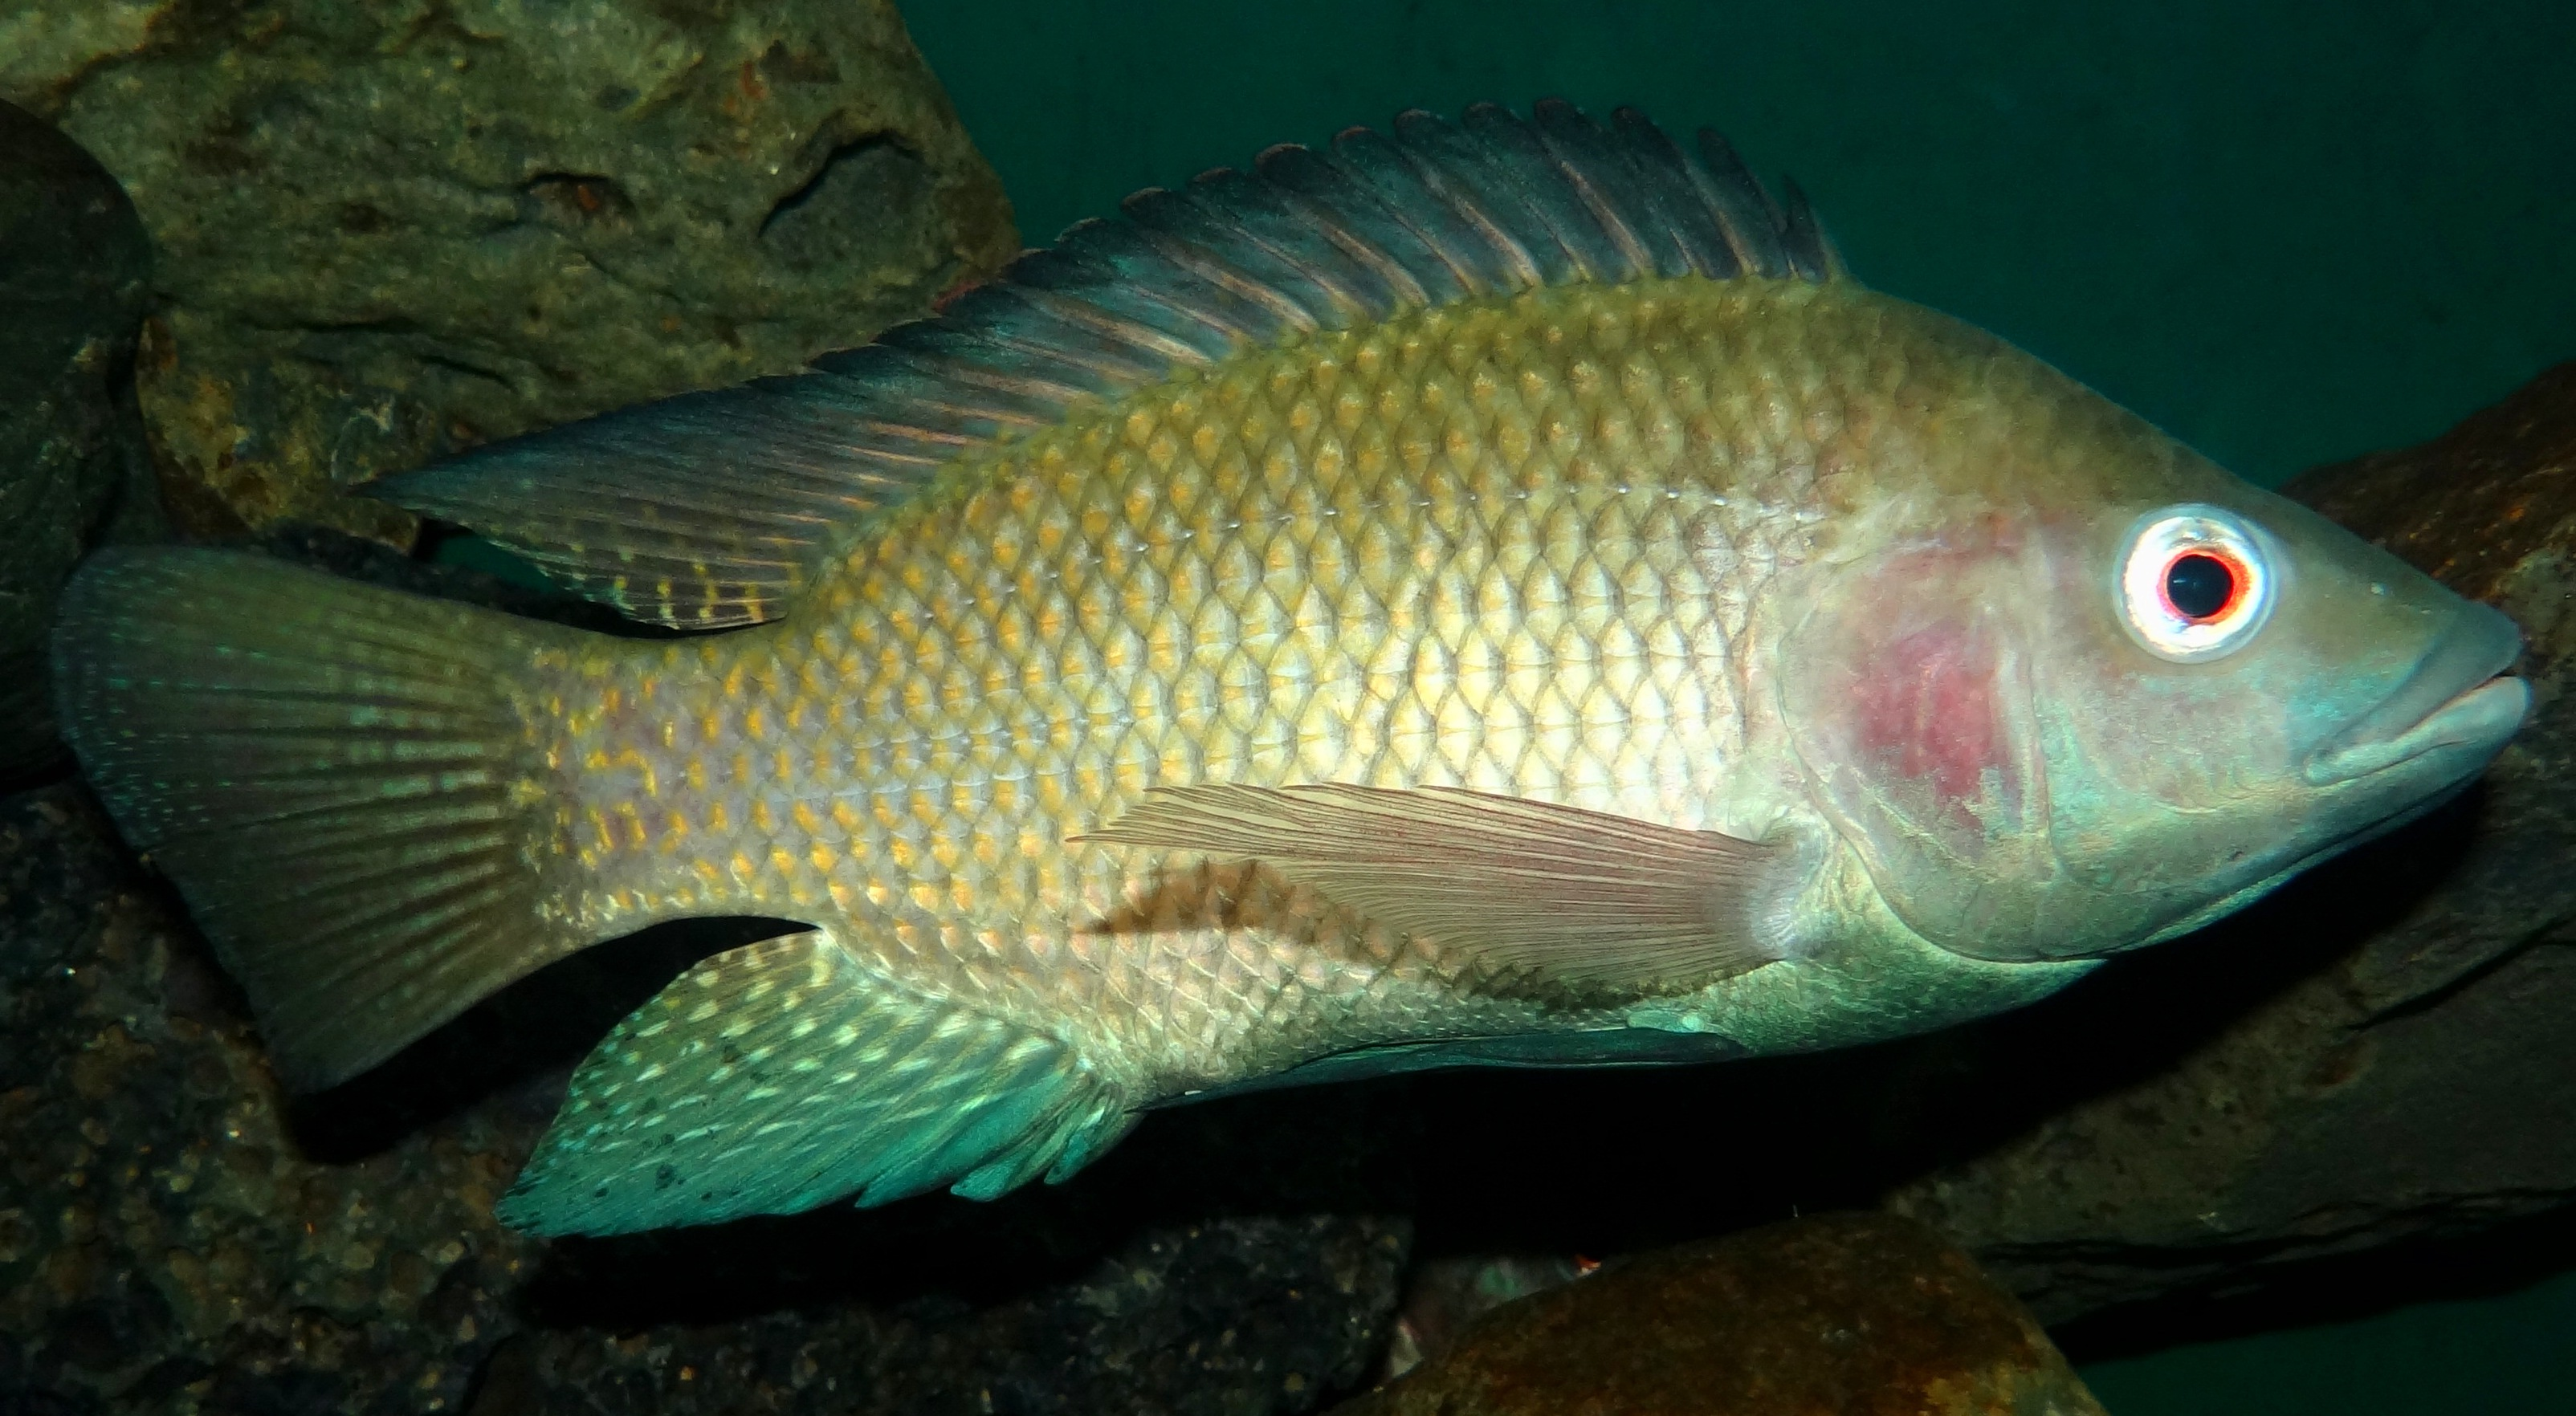
\includegraphics{images_species/Oreochromis-niloticus-Nairobi.jpg}

\textbf{First description}\\
\emph{Oreochromis niloticus} was first described by {[}Linnaeus in 1758
who named it Perca nilotica, this was changed to the current name by
Greenwood, P. H. 1960{]} in his publication which revised the Lake
Victoria Haplochromis species
(\url{https://www.gbif.org/species/4285694}).

\hypertarget{scientific-research-on-the-species-in-the-asean-region-2}{%
\subsection{Scientific Research on the Species in the ASEAN
Region}\label{scientific-research-on-the-species-in-the-asean-region-2}}

\textbf{Research categories}\\
Much of the research on \emph{Oreochromis niloticus} is categorised as
Fisheries (78), Marine and Freshwater Biology (61), Veterinary Sciences
(14), Agriculture, Dairy and Animal Science (11).\\
\textbf{Research summary}\\
The research literature on \emph{Oreochromis niloticus} is largely
concerned with improving productivity of the aquaculture industry that
grows tilapia commercially. Methods of aquaculture are investigated:
such as factors effecting rice polyculture, brackish water aquaculture
and cage aquaculture. Rice polyculture involving the farming of
\emph{Oreochromis niloticus} amongst other fish species in paddy fields
(10.1016/S0044-8486(02)00005-4) has several elements for investigation
including rice seeding rate (10.1016/S0044-8486(98)00396-2), nitrogen
cycling (10.1007/s10705-007-9106-6) and the ecological/economic benefits
of this form of polyculture.

Brackish water aquaculture requires salinity tolerance, which is not a
feature of \emph{Oreochromis niloticus} - it is the least salt tolerant
tilapia, but has a quick growth rate. \emph{O.niloticus} is increasingly
being cultured in coastal ponds (especially in the Philippines,
Indonesia and Vietnam) - sometimes with shrimps - so it would be
beneficial if a more salt tolerant hybrid could be produced
(10.1016/j.aquaculture.2005.02.008).

Stocking density of \emph{O.niloticus} in cages was investigated by the
Asian Institute of Technology in Thailand
(10.1016/S0044-8486(96)01377-4). The combined net yield of both caged
and open-pond tilapia was found to be highest in the treatment with 50
fish m(-3).

The feed used in the aquaculture of \emph{O.niloticus} is the focus of
much research effort, including the replacement of fish oil with
vegetable oil (10.1007/s11745-007-3057-1) - which gave worse yields,
however using cheap farm waste -mushroom stalks -to replace rice bran in
feeds gave a greater yield for less money (Bahari, I. te al 2014).
Scientists supplementing \emph{O.niloticus} feed with antimicrobial
herbal extracts found no mortality in S. agalactiae infected Nile
tilapia for fish receiving dried matter of A. paniculata aqueous extract
supplemented feeds at ratios (w/w) of 4:36 and 5:35
((10.1016/j.jbiosc.2009.01.024). Probiotic supplemented feeds were found
to increase survival in \emph{O.niloticus} infected with \emph{Aeromonas
hydrophila} (Areechon, N. et al 2016).

Infections of fish with pathogens in intensively farmed aquaculture
environments can lead to mass mortality and economic loss, hence much of
the literature is concerned with understanding pathogens, and methods of
combating losses. Intensive \emph{O.niloticus} egg incubation creates
conditions favourable for microbe growth leading to mass mortalities of
fish larvae (Jantrakajorn, S. and Wongtavatchai, J. 2015). Scientists
studied the immune response of \emph{O.niloticus} to better understand
how to develop vaccines (Bunyatratchata, W. et al 2015). Occurrence of
infections in cultured populations of \emph{O.niloticus} are studied to
better understand the disease as was the case with a population infected
with Neoechinorhynchus in the Philippines (Paller, V and de la Cruz C
2012 ).

Heavy metal contamination of watercourses containing farmed
\emph{O.niloticus} is a concern in the literature due to heavy industry
waste being released, an and the potential resultant build up in the
flesh of farmed fish eaten by local people (10.1016/j.proenv.2015.10.057
selangor)(10.1111/j.1365-3156.2007.01939.x). Reduction of copper-induced
tissue changes in \emph{O.niloticus} by calcium exposure is beneficial
in reducing effects in marine species(10.1080/15376510903173674).

Many \emph{O.niloticus} farmers produce all-male populations because of
the superior growth rate of males compared to females. The literature
discussed different methods for achieving this such as hormonal sex
reversal(Guerrero, R.D. 2008), as well as genetic manipulation to create
YY male broodstock achieving a 95.6\% male sex ratio in the
population(10.1139/cjfas-54-2-396).

Understanding the genetic make up of different breeds of
\emph{O.niloticus} (10.1508/cytologia.78.9), and selective breeding
using different strains to genetically improve broodstock - is the focus
of some researchers (10.1016/S0044-8486(97)00230-5).Red Tilapia a strain
of \emph{O.niloticus} bred for its white flesh is a popular strain for
culture.

\textbf{Aquatic or marine?}

Native to the Nile basin rivers and lakes in Africa and coastal rivers
of Israel{]} \emph{O.niloticus} is primarily a freshwater
fish(\url{http://eol.org/pages/356343/data?toc_id=4\#1448}). However
brackish water aquaculture is on the rise in Philippines, Indonesia and
Vietnam which culture \emph{O.niloticus} - which requires salinity
tolerance - not a strength of \emph{Oreochromis niloticus}, as it is the
least salt tolerant cichlid fish, but has a quick growth rate; research
is being conducted to breed a more salt tolerant hybrid of
\emph{Oreochromis niloticus} (10.1016/j.aquaculture.2005.02.008).

\textbf{Is there a description of any research locations that you can
identify?}\\
\emph{O.niloticus} is farmed in its native African countries, and Israel
but has also been exported for aquaculture in fresh and brackish water
locations across the world including: Egypt, Thailand, Philippines,
Indonesia, Malaysia, Vietnam, and Bangladesh.

Some more specific locations are mentioned in the literature such as a
study sampling the fish pathogen \emph{Aeromonas hydrophila} occurrence
in the \emph{O.niloticus} population in West Bay of Laguna de Bay,
Barangay Bayanan, Muntinlupa City, Malaysia in three months during 2005
(Cabrera E. et al.~2006), similarly another study sampled a population
in Sampaloc Lake, Philippines for the occurrence of a fish pathogen
called `Neoechinorhynchus'(Paller, V. and De la Cruz, C. 2012).
Polyculture of \emph{O.niloticus} with `bleeker' was the focus of a
study in the Mekong delta Vietnam. Heavy metal incidence was
investigated in two separate studies in Indonesia one sampling the Galas
River \& Beranang mining pool, Selangor(10.1016/j.proenv.2015.10.057);
and another sampling Lake Cirata, West Java(10.1196/annals.1454.037).
Nitrogen cycling in rice fish culture in Bangladesh, was the subject of
a study (10.1007/s10705-007-9106-6).Spawning season was studied in two
lakes in the Cote d'Ivoire (10.1023/A:100758801082). The spatio-temporal
dynamics of fish larvae in Sirindhron Reservoir, Lower Mekong Basin,
north-east Thailand (10.21077/ijf.2016.63.3.54491-02).

\hypertarget{patent-activity-5}{%
\subsection{Patent activity}\label{patent-activity-5}}

\href{https://www.lens.org/lens/patent/US_6192833_B1}{A partitioned
aquaculture system for \emph{O.niloticus} and other marine organisms,
with an algal channel to control flow rate in the system} is the
invention associated with \emph{O.niloticus} that has been cited most
often.

\href{https://www.lens.org/lens/patent/US_2015_0223495_A1}{The
preparation and use of methionylmethionine as feed additive for fish and
crustaceans} is the patent document associated with \emph{O.niloticus}
with the largest patent family.

\href{https://www.lens.org/lens/collection/24913}{Lens collection}

\hypertarget{penaeus-mondon}{%
\section{\texorpdfstring{\emph{Penaeus
mondon}}{Penaeus mondon}}\label{penaeus-mondon}}

\begin{itemize}
\tightlist
\item
  \textbf{Species name:} \emph{Penaeus monodon}\\
\item
  \textbf{Kingdom:} Animalia\\
\item
  \textbf{Phylum:} Arthropoda
\end{itemize}

\textbf{Brief Description of the Species:}\\
\emph{Penaeus monodon}, the Giant Tiger Prawn, is one example of a group
of giant prawn species with economical importance to the commercial
fisheries industry
\href{https://decapoda.nhm.org/pdfs/25756/25756.pdf}{(L.B.Holthius
(1949))}. The total catch reported for this species for 1999 was 144 042
t with the largest catches from India (93 830t) and Indonesia (31 510 t)
\href{http://www.fao.org/fishery/species/3405/en}{FAO.org}. \emph{P.
monodon} lives in marine (adults) and estuarine (juveniles)
environments, between 0-110 metres in depth and grow to a maximum of
336mm in length, weighing 60-130g
\href{http://www.fao.org/fishery/species/3405/en}{FAO.org}. There are
two specimens of \emph{P. monodon} recorded on
\href{http://portal.vertnet.org/o/umzc/vertebrates?id=urn-catalog-umzc-vertebrates-i-55155}{vertnet},
both are held at the University Museum of Zoology Cambridge and were
collected in India - one specifies the Madras region.

\textbf{Known Distribution of the Species}\\
``Indo-West Pacific: E. and S.E. Africa and Pakistan to Japan, the Malay
Archipelago and northern Australia''
\href{http://www.fao.org/fishery/species/3405/en}{(L.B.Holthius
(1980))}.

\textbf{First description}\\
Penaeus monodon was first described by Johan Christian Fabricus in 1798,
but clarification of which species this name referred to came later in
1949, when Lipke Holthuis showed it to be the type species of the genus
\emph{Penaeus}
\href{https://decapoda.nhm.org/pdfs/25756/25756.pdf}{(L.B.Holthius
(1949))}.

\begin{figure}
\centering
\includegraphics{images_species/CSIRO_ScienceImage_2992_The_Giant_Tiger_Prawn.jpg}
\caption{CSIRO}
\end{figure}

\hypertarget{scientific-research-on-the-species-in-the-asean-region-3}{%
\subsection{Scientific Research on the Species in the ASEAN
Region}\label{scientific-research-on-the-species-in-the-asean-region-3}}

\textbf{Research categories}\\
Much of the research on \emph{P.monodon} is categorised as fisheries
(288), followed by Marine and Freshwater Biology (179), Veterinary
Sciences (123), Immunology (81), Zoology (60), Biochemistry \& Molecular
Biology (58), Biotechnology and Applied Microbiology (45), Virology (32)
and so on.

\textbf{Research summary}\\
The majority of the research effort on \emph{P.monodon} is directed
towards maximising fisheries yield and increasing economic gain. As such
a lot of the \emph{P.monodon} literature is concerned with understanding
the immune response of the shrimp populations to the main viral and
bacterial pathogens which cause large scale mortality in the population,
such as White Spot Syndrome Virus (WSSV), Yellow Head Virus (YHV) and
\emph{Vibrio harveyi}(10.1016/j.fsi.2011.10.013)
(10.1016/j.dci.2012.09.001). Whilst others are focussed on improving
shrimp reproduction for example injecting female broodstock with a
hormone that stimulates the ovaries (10.1016/j.aquaculture.2015.04.027
shrimp repro). Some work is concerned with identifying sub-populations
of P. monodon where there is significant genetic differentiation between
samples collected from different geographic areas ((Jarayabhand, P et al
2000).

\textbf{Aquatic or marine?}\\
\emph{P. monodon} is fished from wild populations in offshore marine
waters, however there is reference to inshore and pond fishing in some
countries: Singapore, Malaya, Philippines, Thailand and Vietnam
\href{http://www.fao.org/fishery/species/3405/en}{(L.B.Holthius (1980))}
(10.1111/jwas.12423). In addition juveniles live in river mouth and
estuarine mangrove environments predominantly - which act as a nursery
with adults living in deeper offshore environments. Wild marine
populations are commonly used to establish disease free broodstock for
commercial pond fisheries inland (10.1016/j.aquaculture.2010.08.015).
Thus some of the research is solely focussed on captive inland
populations from commercial farms (10.1007/s11259-010-9434-x) whilst
others are comparative studies between wild and captive specimens.

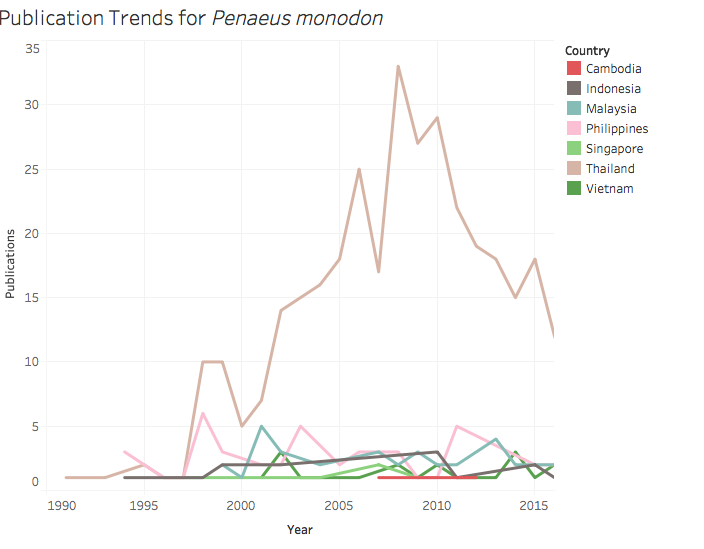
\includegraphics{images_species/country tends p_mondonpng.png}

\textbf{Is there a description of any research locations that you can
identify?}\\
Much of the research involves laboratory bred broodstock of \emph{P.
monodon}, but from different geographical populations, where often only
the country is cited: Australia, China, Taiwan, Malaysia, Vietnam,
Thailand, Papua New Guinea, New Caledonia, India, Singapore,
Philippines, Tanzania, Japan, Sulawesi, Sumatra, and Brazil. There are
some references to more specific locations within the literature such as
research in the Mekong Delta Region of Southern Vietnam looking at
different pond farming methods - including mangrove ponds
(10.1080/13657305.2013.747224).Similarly another study investigated
\emph{P.monodon} overfishing by artisanal fishermen in the Saadan
Estuary in Tanzania, again an area with mangroves
(10.1016/j.ocecoaman.2013.05.003). The Brunei waters of the South China
Sea are the location mentioned in a study seeking disease free
broodstock for inland shrimp farms (10.1016/j.aquaculture.2010.08.015).
A study investigating genetic variation amongst \emph{P.monodon} from 5
geographic locations within Thai waters lists: Chumphon and Trad within
the Gulf of Thailand, as well as Phangnga, Satun, and Trang within the
Andaman Sea (Jarayabhand, P et al 2000).Another genetic diversity study
on P. monodon cites samples taken from the coastal waters of Qinglan
(Hainan Province of China) and Malaysia (Li Shaojing et al 2008). Joseph
Bonaparte Gulf in northern Australia was cited in a study on a new 7th
genotype of YHV to infect shrimp ponds in Australia
(10.3354/dao02894).South western and south eastern Indian coastal
populations of farmed shrimps are used in a disease study of P.monodon
(10.3354/dao01835).

\hypertarget{patent-activity-6}{%
\subsection{Patent activity}\label{patent-activity-6}}

The top cited patent document involving \emph{P. monodon} is for a
\href{https://www.lens.org/lens/patent/US_4055145_A}{dual purpose
installation} - whereby a system converts ocean thermal energy into
electrical energy, at the same time the system benefits a lagoon
population of \emph{P.monodon} which are reared for the food industry.
The system involves pumping cold deep sea water - which is nutrient rich
to cool the working fluid and condense it, the surface water warms the
working fluid and evaporates it. The closed cycle converts heat energy
to electricity and the shrimps benefit from the nutrient rich deep
seawater.

The cited example of a suitable location in the patent document is the
Lime Island chain 1000 miles south of Hawaii, with the Philippine Tiger
Prawn \emph{P.monodon} being used. It doesn't specify utilising samples
of \emph{P.monodon} when inventing the system which is included in this
document.

The second most cited patent document involving P.monodon is for a
\href{https://www.lens.org/lens/patent/US_6571735_B1}{non metallic
bioreactor}, suitable for unicellular or multicellular culture - with
\emph{P.monodon} being one of the listed species that could be farmed
within it. There is no location specified for this patent as it is a
bioreactor design.

\href{https://www.lens.org/lens/patent/WO_2008_084074_A2}{Specialised
Feed composition for aquatic organisms} including larvae of \emph{P.
monodon}. Similarly to above there is no location specified for this
patent document.

\href{https://www.lens.org/lens/patent/US_2005_0080032_A1}{This patent
is for methods of delivering dsRNA into invertebrate marine organisms
such as shrimps, to illicit an immune response}. This includes methods
of delivery of the dsRNA i.e.~whether it is injected, ingested in a feed
medium, or placed within an algae that is ingested.In addition methods
of identifying genes in invertebrates that are involved in immune
responses are also included.

\href{https://www.lens.org/lens/collection/24679}{Lens Collection}

\hypertarget{pomacea-canaliculata}{%
\section{\texorpdfstring{\emph{Pomacea
canaliculata}}{Pomacea canaliculata}}\label{pomacea-canaliculata}}

\begin{itemize}
\tightlist
\item
  \textbf{Species name:} \emph{Pomacea canaliculata}
\item
  \textbf{Kingdom:} Animalia
\item
  \textbf{Phylum:} Mollusca
  \href{https://www.gbif.org/species/2292582}{GBIF}
\end{itemize}

\textbf{Brief Description of the Species:}\\
\emph{Pomacea canaliculata} is a freshwater snail with a voracious
appetite for water plants including lotus, water chestnut, taro and
rice. Introduced widely from its native South America by the aquarium
trade and as a source of human food, it is now a major crop pest in
south east Asia (primarily in rice) and Hawaii (taro) and poses a
serious threat to many wetlands around the world through potential
habitat modification and competition with native species. A highly
generalist and voracious macrophytophagous herbivore. Most plants are
eaten (\url{http://www.iucngisd.org/gisd/species.php?sc=135}).

The activity rate of \emph{Pomacea canaliculata} varies highly with the
water temperature. At 18°C they hardly move around, whilst the opposite
is true at higher temperatures e.g.~25°C (The
(\url{http://www.iucngisd.org/gisd/species.php?sc=135}).

Females lay clusters of bright pink eggs attached to solid surfaces and
reproductive output can be enormous with clutch sizes of up to 1000, but
averages are probably 200-300. Clutches are laid every few weeks
(\url{http://www.iucngisd.org/gisd/species.php?sc=135}).

\begin{figure}
\centering
\includegraphics{images_species/Pomacea_canaliculata_01.jpg}
\caption{By H. Zell (Own work)}
\end{figure}

\textbf{Known Distribution of the Species}\\
\emph{P. canaliculata} is native from Argentina to the Amazon basin, as
well as being introduced to most of southern, eastern, and southeast
Asia and the southern part of the United States
(\url{http://eol.org/pages/467346/overview}). \emph{P. canaliculata} is
widely distributed in lakes, ponds and swamps throughout its native
range of the Amazon Inferior Basin and the Plata Basin
(\url{http://www.iucngisd.org/gisd/species.php?sc=135}).

Biogeographic Regions: nearctic (Introduced ); oriental (Introduced );
neotropical (Native); oceanic islands (Introduced
)(\url{http://eol.org/pages/467346/overview}).

\textbf{First description}\\
The French Biologist Jean Baptiste Lamarck first described \emph{P.
canaliculata} in the natural history of invertebrates in 1822
(\url{https://www.gbif.org/species/2292582}).

\hypertarget{scientific-research-on-the-species-in-the-asean-region-4}{%
\subsection{Scientific Research on the Species in the ASEAN
Region}\label{scientific-research-on-the-species-in-the-asean-region-4}}

\textbf{Research categories}\\
Much of the research on \emph{Pomacea canaliculata} is categorised as
Agronomy (7), Biotechnology and Applied Microbiology (4), Entomology
(4), Environmental Sciences (4), Toxicology (4), Agriculture,
Multidisciplinary (3).

\textbf{Research summary}

Much of the research on \emph{Pomacea canaliculata} is concerned with
ways to effectively control the invasive pest in agricultural settings,
including the use of fish predators in rice fields
(10.1016/j.cropro.2006.01.012), as well as molluscicides (De la Cruz,
M.S. and Joshi, R.C.2001). Quinoa saponins a natural molluscicide were
found to be an effective environmentally friendly alternative to
synthetic molluscicides at eradicating \emph{Pomacea canaliculata},
especially in direct seeded cultures of rice
(10.1016/j.cropro.2007.08.010). In a study in Thailand natural pathogens
of \emph{Pomacea canaliculata} were isolated from the soil - strains of
\emph{Pseudomonas aeruginosa} and \emph{P. fluoescens}
(10.1023/B:WIBI.0000007312.97058.48).

The human health risk posed by \emph{Pomacea canaliculata} with regard
to its transmission of parasites was the focus of several studies which
monitored snail populations in aquatic bodies near populated areas. One
study examined the effect of the building of a dam in central Laos PDR
on numbers of all snails including \emph{Pomacea canaliculata} - the
intermediate host of \emph{A.cantonensis}- it was the snail species
found in the greatest numbers during 2010 and 2011; numbers increased
greatly from 1.3\% in 2010 to 53.3\% in 2011 (Brey, P.T. 2015).

In 2006/7 tsunami and non-tsunami affected areas of Takua Pa District,
Phang-Nga Province were examined for snails that transmit human
parasitic diseases - 16 species were identified including \emph{Pomacea
canaliculata}. Knowledge of these medically important snails and their
parasitic diseases, and prevention were given to Takua Pa people
(Butraporn, P. 2010).

Another public health focus of the literature regarding \emph{Pomacea
canaliculata} concerned their potential use as biomonitors in waterways
which could be subject to heavy metal pollution. This was shown to
effect the tissues of the snails in an observable manner at levels below
the safety limit, at a lake in Thailand (10.1016/j.ecoenv.2012.09.018).
Similarly another study focussed on the effect of copper sulphate
exposure on the tissue of \emph{Pomacea canaliculata}, they also found
the snail to be an effective potential bioindicator of copper
contamination in aquatic environments (10.1016/j.ecoenv.2015.08.010).

A better understanding of the general biology of \emph{Pomacea
canaliculata} led some researchers to look at its life cycle (Arfan, A.
et al 2015), whilst others examined genetic diversity (Bai, Xu et al
2011) and some specifically looked at tolerance of different climatic
populations to dessication and cold (10.1093/mollus/eyq049).

Differing cultivation methods were examined to note any effect on the
mortality rate of rice due to \emph{Pomacea canaliculata} infested
ponds. One study noted that planting out 21 days after sowing gave a
greater chance of survival for the rice seedlings
(10.1016/j.cropro.2014.06.022).

\textbf{Aquatic or marine?} Although \emph{Pomacea canaliculata} is
largely a freshwater snail, reference is made to them occupying, marsh,
swamp and marine habitats (\url{http://eol.org/pages/467346/overview}).

\textbf{Is there a description of any research locations that you can
identify?}

Snails in Beung Boraphet reservoir, Nakhon Sawan Province, central
Thailand were examined in a study of metal pollution
(10.1016/j.ecoenv.2012.09.018). Areas of Takua Pa District, Phang-Nga
Province were investigated for fresh- and brackish-water snails that
transmit human parasitic diseases during 2006 and 2007 (Butraporn, P.
2010). Another study in Thailand looked at natural microbe pathogens in
the soil (10.1023/B:WIBI.0000007312.97058.48).

The Philippines is the location of a couple of studies including one on
rice cultivation methods to reduce mortality
(10.1016/j.cropro.2014.06.022), and a molluscicide study in Munoz, Nueva
Ecija (De la Cruz, MS. and Joshi, RC 2001), as well as a genetic
diversity analysis using a population from Los Banos (Bai, X. et al
2011).

The effect of building a dam on the snail population was investigated at
Khammouane Province, central Laos (Brey, P.T. 2015).

China (Yuyao, Taizhou, Fuzhou, Guangzhou, Nanning, Kunming) (Bai, Xu et
al 2011), Japan (Kyushu and Luzon Mindanao) (10.1093/mollus/eyq049) and
Taiwan are also mentioned within the research literature (Baker, GH.
1998).

\hypertarget{patent-activity-7}{%
\subsection{Patent activity}\label{patent-activity-7}}

There are 114 patent documents for \emph{Pomacea canaliculata}, the most
commonly cited patent document is for a modified plant chemical called
`saponin' that can be used to kill these molluscs in areas where they
are considered a pest
\href{https://www.lens.org/lens/patent/US_2007_0196517_A1}{US20070196517A1}.

\href{https://www.lens.org/lens/collection/24984}{Lens collection}

\hypertarget{vibrio-harveyi}{%
\section{\texorpdfstring{\emph{Vibrio
harveyi}}{Vibrio harveyi}}\label{vibrio-harveyi}}

\begin{itemize}
\tightlist
\item
  \textbf{Species name:} \emph{Vibrio harveyi}
\item
  \textbf{Kingdom:} Bacteria\\
\item
  \textbf{Phylum:} Proteobacteria
  \href{https://www.gbif.org/species/5427692}{GBIF}
\end{itemize}

\textbf{Brief Description of the Species:}\\
\href{http://eol.org/pages/973242/details}{\emph{Vibrio harveyi}}, is a
Gram-negative, bioluminescent, common marine bacterium in the same genus
as \emph{Vibrio parahaemolyticus}. \emph{V. harveyi} is rod-shaped and
can be found free-swimming in tropical marine waters, living commensally
in the gut microflora of marine animals, a minority of \emph{V.harveyi}
strains are pathogenic to marine animals, including Gorgonian corals,
oysters, prawns, lobsters, the common snook, barramundi, turbot,
milkfish, and seahorses. It is responsible for luminous vibriosis, a
disease that affects commercially farmed penaeid prawns such as
\emph{P.monodon}. Additionally, based on samples taken by ocean-going
ships, V. harveyi is thought to be the cause of the {[}milky seas
effect{]}
(\url{https://www.nrl.navy.mil/media/news-releases/2005/nrl-scientists-detect-milky-sea-phenomena}),
in which, during the night, a uniform blue glow is emitted from the
seawater. Some glows can cover nearly 6,000 sq mi (16,000 km2)
(\url{http://eol.org/pages/973242/details}).

\emph{V. harveyi} related strains have been isolated from the deep sea
\textgreater{}1000m2, these may be ecologically differentiated strains,
adapted to a different ecological niche or be distributed across the
oceans (Thompson and Austin 2006).

Although normally a benign bacteria in marine cultured environments, the
prevalence of the pathogenic strains of \emph{V. harveyi} - that differ
by a few pathogenic determinant genes - can cause a problem in high
nutrient, high density conditions leading to a rapid spread of virulent
strains (Ben-Haim et al., 2003).

Although closely related to the human pathogen \emph{V.
parahaemolyticus}, \emph{V. harveyi} is not known as a
\href{https://www.ncbi.nlm.nih.gov/genome?term=txid669\%5Borgn\%5D}{human
pathogen}. This is one of the first organisms in which {[}quorum
sensing{]}
(\url{https://www.ncbi.nlm.nih.gov/genome?term=txid669\%5Borgn\%5D}) was
described, whereby communities of bacteria communicate with each other
via secreted signalling molecules synchronising community behaviour by
regulating gene expression - both within and between bacteria species.

\textbf{Known Distribution of the Species}\\
Vibrio harveyi is a common bacteria inhabiting largely tropical marine
waters - as it requires sodium chloride
(10.1111/j.1472-765X.2006.01989.x), and prefers warmer water
temperatures.

\textbf{First description}\\
\emph{Vibrio harveyi} was named by Baumann et al.~in 1981, further to
the work of Johnson \& Shunk, 1936 who originally named the species
\emph{Achromobacter herveyi}.
\href{https://www.gbif.org/species/5427692}{GBIF}

\hypertarget{scientific-research-on-the-species-in-the-asean-region-5}{%
\subsection{Scientific Research on the Species in the ASEAN
Region}\label{scientific-research-on-the-species-in-the-asean-region-5}}

\textbf{Research categories}\\
Much of the research on \emph{Vibrio harveyi} is categorised as
Fisheries (72), Marine and Freshwater Biology (44), Veterinary Sciences
(37), Immunology (30), Microbiology (24), Biotechnology and Applied
Microbiology (23) and Biochemistry and Molecular Biology (19).

\textbf{Research summary}\\
The research effort on \emph{Vibrio harveyi} is largely concerned with
infection of fish, molluscs and crustaceans within the aquaculture
industry. As such a lot of the \emph{V. harveyi} literature is concerned
with understanding the pathogenic strains of the bacteria that infects
commercially farmed marine organisms, particularly shrimps: methods of
rapidly detecting V.harveyi infections (2672.2003.02020.x),
antimicrobial peptides produced by marine organisms that could combat
\emph{V.harveyi} (10.1016/j.aquaculture.2009.01.026) and naturally
occurring compounds that have antimicrobial properties against
\emph{V.harveyi} whilst being safe to cultured marine
organisms(10.1111/are.13043). Shrimps infected with \emph{V. harveyi}
produce an antimicrobial peptide that has been shown to be effective in
combating the bacteria when administered into a culture or injected into
shrimps(10.1016/j.aquaculture.2009.01.026).

Overuse of antibiotics in aquaculture is blamed for an increase in
antibiotic resistant strains of bacteria (10.1016/j.fm.2016.02.008), so
\emph{V.harveyi} researchers are looking at alternative methods of
combating the bacteria, including the use of novel natural compounds
found in cyanobacteria(10.1111/are.13043) and extracts from
\emph{Sargassum oligocystum} (Apines-Amar, MJS. et al., 2011).

\textbf{Aquatic or marine?}\\
\emph{Vibrio harveyi} is found in marine and estuarine waters, however
its presence has also been noted in Giant Freshwater Prawn larvae which
inhabit brackish water as juveniles and freshwater as
adults(10.1016/j.aquaculture.2013.05.015).

\textbf{Is there a description of any research locations that you can
identify?}\\
Much of the research referencing specific locations for \emph{V.harveyi}
is from investigations into the cause of aquaculture shrimp mortalities
as was the case in pond-cultured Penaeus monodon in the provinces of
Bohol, Misamis Occidental, Lanao del Norte and Zamboanga del Sur,
Philippines (Inui, Y. et al., 2003). Similarly dead shrimp larvae from
hatcheries in Jepara, Indonesia(10.1016/0044-8486(94)00374-W), Southern
Thailand (10.3354/dao035195), and Iran (Afsharnasab, M. et al., 2014)
were found to contain \emph{V.harveyi}. Seasonal changes in the
composition of a variety of vibrio species including \emph{V.harveyi}
were investigated in samples taken from Yoshimi Bay, Hibiki-nada Sea,
Japan.

\hypertarget{patent-activity-8}{%
\subsection{Patent activity}\label{patent-activity-8}}

\href{https://www.lens.org/lens/patent/US_6551795_B1}{Nucleic acid and
amino acid sequences relating to pseudomonas aeruginosa for methods for
the detection, prevention and treatment of pathological conditions
resulting from bacterial infection including \emph{V.harveyi}}.

\href{https://www.lens.org/lens/patent/US_2007_0212727_A1}{Microorganisms
for therapy wherein the microorganisms gather in inflamed or cancerous
tissues and cause cells to become leaky, resulting in production of
antibodies, one such type of microorganism is attentuated Vibrio}

\href{https://www.lens.org/lens/collection/24872}{Lens collection}

\hypertarget{vibrio-parahaemolyticus}{%
\section{\texorpdfstring{\emph{Vibrio
parahaemolyticus}}{Vibrio parahaemolyticus}}\label{vibrio-parahaemolyticus}}

\begin{itemize}
\tightlist
\item
  \textbf{Species name:} \emph{Vibrio parahaemolyticus}
\item
  \textbf{Kingdom:} Bacteria\\
\item
  \textbf{Phylum:} Proteobacteria
  \href{https://www.gbif.org/species/5427673}{GBIF}
\end{itemize}

\textbf{Brief Description of the Species:}\\
\emph{Vibrio parahaemolyticus}, is a gram negative bacteria that is
found in estuarine, coastal and marine waters
\href{https://www.ncbi.nlm.nih.gov/pmc/articles/PMC4263241/}{Letchumanan
et al 2014} and is present in higher concentrations between May and
October when temperatures are warmer
\href{https://www.cdc.gov/vibrio/faq.html}{CDC}. \emph{V.
parahaemolyticus} responsible for the disease vibriosis in humans,
contracted through eating raw contaminated shellfish such as oysters, or
exposure of a wound to infected salt or brackish water
\href{https://www.cdc.gov/vibrio/faq.html}{CDC}. \emph{V.
parahaemolyticus} is found in a free swimming state, using a single
flagellum to attach to zooplankton, fish, shellfish or suspended matter
in the water
\href{https://www.ncbi.nlm.nih.gov/pmc/articles/PMC4263241/}{Letchumanan
et al 2014}(10.3389/fmicb.2014.00705). The prevalence of the pathogenic
strains of \emph{V. parahaemolyticus} isolated from seafood, and
clinical samples shows it to have a worldwide distribution across South
East Asia, Europe, and US posing an ongoing health threat to the
population. Within Asia, samples have been found in seafood in markets
in China, Malaysia, India, Bangladesh, Taiwan, Laos, hong Kong and Japan
\href{https://www.ncbi.nlm.nih.gov/pmc/articles/PMC4263241/}{Letchumanan
et al 2014}(10.3389/fmicb.2014.00705).

\textbf{Known Distribution of the Species}\\
``Present in the Gulf of Mexico''
\href{http://www.gbif.org/species/5427673}{GBIF}.

\textbf{First description}\\
\emph{Vibrio parahaemolyticus} was named by Sazaki et al.in 1963,
further to the work of Fujino et al.~in 1951 who originally named the
species \emph{Pasteurella parahaemolytica}
\href{https://www.gbif.org/species/5427673}{(GBIF)}.

\begin{figure}
\centering
\includegraphics{images_species/Vibrio_parahaemolyticus_01 copy.png}
\caption{Janice Carr/CDC}
\end{figure}

\hypertarget{scientific-research-on-the-species-in-the-asean-region-6}{%
\subsection{Scientific Research on the Species in the ASEAN
Region}\label{scientific-research-on-the-species-in-the-asean-region-6}}

\textbf{Research categories}\\
Much of the research on \emph{Vibrio parahaemolyticus} is categorised as
Microbiology (60), Food Science and Technology (30), Biotechnology and
Applied Microbiology (29), Fisheries (29), Veterinary Sciences (21),
Infectious diseases (19), Marine and Freshwater Biology (17), Immunology
(11) and so on.

\textbf{Research summary}\\
The research effort on \emph{Vibrio parahaemolyticus} is largely
concerned with infection of fish, molluscs and crustaceans within the
aquaculture industry, as well as infection of humans that eat infected
seafood. As such a lot of the \emph{V. parahaemolyticus} literature is
concerned with understanding the pathogenic strains of the bacteria that
infects humans and commercially reared seafood including: methods of
rapidly detecting strains causing an infection
(10.1017/S0950268806006017), vaccines offering protection
(10.1016/j.vaccine.2011.04.021) and ways of treating the infection.
Shrimps infected with \emph{Vibrio parahaemolyticus} can develop acute
hepatopancreatic necrosis disease causing severe mortalities in SE Asia
and Mexico, some research has been directed to noting any genetic
difference between bacterial infections from different geographical
areas.

Overuse of antibiotics in aquaculture is blamed for an increase in
antibiotic resistant strains of \emph{Vibrio parahaemolyticus}
(10.1016/j.fm.2016.02.008), so researchers are also looking at
alternative methods of combatting the bacteria: including the use of
bacteria phage - such as one discovered in Laos (Higa, N. et al 1999).
In ensuring people don't become sick from eating seafood, some research
has been focussed on food preservatives that extend the life of seafood
because of their inhibitory effect on \emph{Vibrio parahaemolyticus}such
as botanical extracts from \emph{Terminalia chebula} (Kaewmanee,P et al
2012) and \emph{Zingiber spectabile}(10.1016/j.foodcont.2012.09.012),
and best practice for safe processing of seafood
(10.1016/j.foodcont.2012.02.009). There are many studies noting the
range of strains present in certain geographic areas, in Taiwan and 14
other countries 535 strains were identified of \emph{Vibrio
parahaemolyticus} (10.1016/j.ijfoodmicro.2006.09.024) - either by
testing samples of infected faeces of people from clinical settings,
(10.1099/jmm.0.47439-0) or sampling water and noting the strains of
\emph{Vibrio parahaemolyticus} present. Certain strains are given more
attention, as they are more virulent, pathogenic and novel - so there is
little resistance in the local human population - it is these strains,
such as the pandemic strain, that are of more concern in the literature.

\textbf{Aquatic or marine?}\\
\emph{Vibrio parahaemolyticus} is found in marine and brackish waters,
however its presence has also been noted in a tropical coastal lagoon
from 2 samples collected in the estuary near Yor Island, Songkhla Lake,
Thailand (10.1139/W11-084).

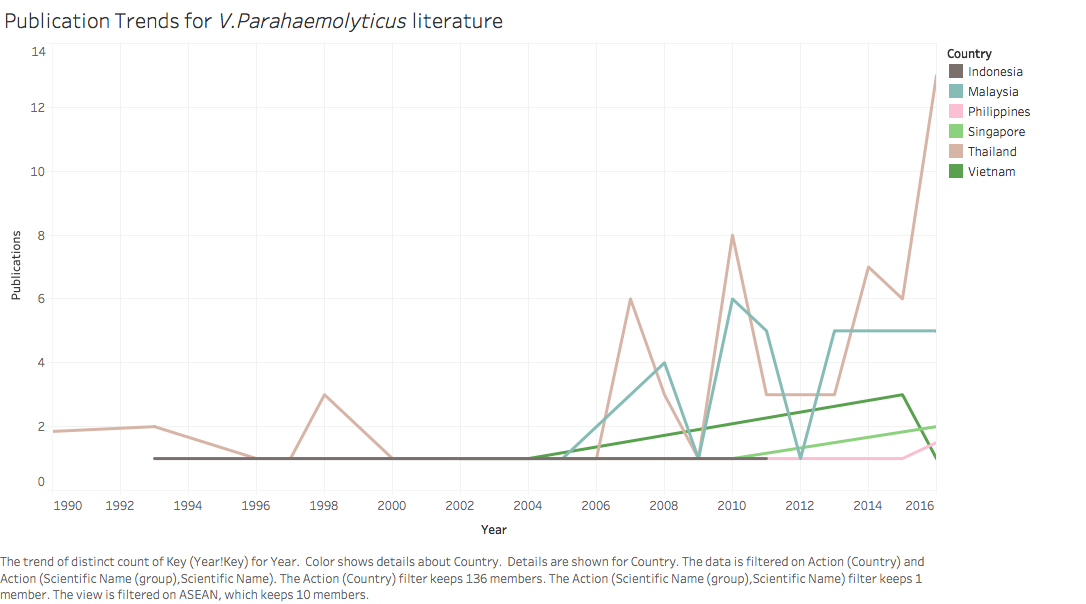
\includegraphics{images_species/publication trends Vibrio para.png}

\textbf{Is there a description of any research locations that you can
identify?}\\
Much of the research involving samples taken from humans infected with
\emph{Vibrio parahaemolyticus} reference a country for \url{example:US},
Italy, Brazil, Philippines, Malaysia, China, India, Thailand, Iran,
South Africa and Australia, (10.1016/j.fm.2016.02.008). Some clinical
studies are more specific in noting a hospital or region: a study
conducted at Hat Yai Hospital in southern Thailand
(10.1099/jmm.0.47439-0) for example, and a similar stool sample study in
the infectious Diseases Hospital in Kolkata, India examining strains
present in infected samples using the PFGE analysis technique to
identify the strains (10.1371/journal.pntd.0002815). Food poisoning
cases in Kangawa Prefecture, Japan were the source of 18 strains of
\emph{V. parahaemolyticus} studied in laboratories in Thailand to note
the specific genes present (10.1007/s002849900188).

Forty two strains of \emph{Vibrio parahaemolyticus} were isolated form
samples of water taken form the estuaries around Bangladesh in the Bay
of Bengal, with some being of the virulent and ptahogenic strains posing
a risk to inhabitants of coastal villeages in the area(42
10.1128/AEM.00266-09). A study on patients with diarrhoea in North
Jakarta, Indonesia, found \emph{Vibrio parahaemolyticus} was responsible
for a substantial number of cases, with incidence being highest in the
dry season (June and July), many of the samples showed antibiotic
resistance to some antibiotics (10.1016/S0732-8893(00)00232-7).

Samples of seafood were analysed from Hong Kong, Indonesia, Thailand and
Vietnam - of the samples taken 45.9\% contained \emph{Vibrio
parahaemolyticus}, with more of teh samples from Hong Kong and Thailand
containing teh bacteria (10.1016/S0168-1605(99)00143-9).

170 strains of \emph{V. parahaemolyticus} were isolated from water
samples collected along the Georgian coast of the Black Sea, water
temperature was shown to be a factor in its presence especially in the
Green cape samples(10.3389/fmicb.2014.00045).

\hypertarget{patent-activity-9}{%
\subsection{Patent activity}\label{patent-activity-9}}

The top cited patent document involving \emph{V. parahaemolyticus} is
for
\href{https://www.lens.org/lens/patent/US_2004_0029129_A1}{identification
of essential genes used to help \emph{V. parahaemolyticus} multiply} - a
sequence of nucleic acids is used to undertsand which are the key
important proteins in the bacteria and then drugs, or antibodies can be
produced to prevent replication of the bacteria.

The patent document with the largest family is for the
\href{https://www.lens.org/lens/patent/WO_2009_043477_A2}{use of a
peptide as a therapeutic agent} when someone has a \emph{V.
parahaemolyticus} infection.

\href{https://www.lens.org/lens/collection/24760}{Lens collection}

\hypertarget{method}{%
\chapter{Annex 2: Methodology}\label{method}}

In this section we describe the basic methodology and data sources used
for the Scientific and Patent Landscape for Marine Genetic Resources in
South East Asia. Methods can be divided into the following categories.

\begin{enumerate}
\def\labelenumi{\arabic{enumi}.}
\tightlist
\item
  Searching the Scientific Literature
\item
  Searching the Patent Literature
\item
  Identifying Species Names
\end{enumerate}

\hypertarget{the-scientific-literature}{%
\section{The Scientific Literature}\label{the-scientific-literature}}

\href{https://clarivate.com/products/web-of-science/web-science-form/web-science-core-collection/}{Web
of Science} from Clarivate Analytics (formerly Thomson Reuters) is a
leading commercial database of scientific literature and is widely
available in Universities. Web of Science covers thousands of journals
across multiple subjects and is made up of a number of databases
available under a range of subscription models. We used the
\href{https://clarivate.com/products/web-of-science/web-science-form/web-science-core-collection/}{Web
of Science (WOS) Core Collection} consisting of data from over 18,000
journals along with conference proceedings. This database is common to
all subscription models for Web of Science (with the others being
optional). Use of the Core Collection therefore assists with the
reproducibility of research. The Core Collection also contains more
detailed fields, for example on author affiliations, than other
databases in the family and is therefore a preferred choice for
bibliometric research.

\hypertarget{searching-web-of-science}{%
\subsection{Searching Web of Science}\label{searching-web-of-science}}

We focused on obtaining scientific literature about the ten ASEAN
countries in two categories:

\begin{enumerate}
\def\labelenumi{\arabic{enumi}.}
\tightlist
\item
  Scientific literature listing an author from the country in the
  Address field of scientific publications.
\item
  Scientific Literature that referenced the country in the Topic Field
  (Titles, Abstracts, Author Keywords and Keywords Plus (titles of cited
  literature))
\end{enumerate}

We searched across all years beginning in 1900 to the period between
late May 2017 and mid-June 2017.

Downloads of Web of Science records were formerly limited to 500 records
per set. Where the number of records exceeded 100,000 we sought to limit
the datasets by Web of Science Subject Categories. Web of Science
Subject Categories describe the \emph{subject areas} of journals in Web
of Science rather than the articles themselves. In selecting the Subject
Categories we focused on those areas with a biological connection and
for traditional knowledge we looked at the social sciences. The Analyze
function in Web of Science permits the ranking of records based on the
subject category and aided in the selection process.

In cases where we refined the data by subject area we typically started
the research by using the Analyze function on subject categories ordered
alphabetically to make the selection. This was limited to the top 100
categories. In a second step we then used the full list to download a
smaller set containing other relevant subject categories. Typically
these were smaller subject areas (such as Entomology or Marine
Engineering) that did not appear in the top 100. To capture data
potentially relevant to traditional knowledge we included social science
subject areas while recognising that the majority of records would not
be relevant.

In cases where datasets were refined by subject category we sought to
cast the net as widely as possible while keeping the results below
100,000.

\hypertarget{overall-trends}{%
\subsection{Overall Trends}\label{overall-trends}}

We obtained an overview of research trends for each category using the
\texttt{Analyze} function in Web of Science to identify the top 500
authors, the top 600 organizations (organizations enhanced), data on
publication years, and the ranked Web of Science Subject Categories.

We then downloaded the results, tidied up the data titles and imported
the files into RStudio. Individual country data was joined using the
dplyr function \texttt{full\_join} for an SQL join. Because the data for
each country varies in length, this joins the tables together on the
subject categories and introduces an NA for Not Available where a
category is missing for an individual field. These files were compiled
in the data folder of the repository as \texttt{asean\_authors},
\texttt{asean\_categiries}, \texttt{asean\_organizations} and
\texttt{asean\_year}.

\hypertarget{patent-data}{%
\section{Patent Data}\label{patent-data}}

Patent Data for the research consisted of three components.

\begin{enumerate}
\def\labelenumi{\arabic{enumi}.}
\tightlist
\item
  PATSTAT
\end{enumerate}

The
\href{https://www.epo.org/searching-for-patents/business/patstat.html\#tab-1}{EPO
World Patent Statistical Database (PATSTAT)} is a statistical database
developed by the European Patent Office in collaboration with OECD and
other partners. It contains the basic content of the core DOCDB database
and has been augmented with additional data tables such as cleaned
assignee names and economic sector tables. As a statistical database
PATSTAT is not suitable for text mining and requires knowledge of SQL.

We used the
\href{http://www.patstat.org/Patstat/PatstatApp/app/index.html\#/disclaimer}{Intelligent
Information Services Corporation (IISC) portal} to access the EPO World
Patent Statistical Database (PATSTAT) Autumn 2016 edition. PATSTAT is a
SQL based database and IISC has the advantage of providing a simplified
interface and directly compiling datasets for use in VantagePoint from
Search Technology Inc.~This considerably simplified the requirements for
using PATSTAT and processing the data but is limited to VantagePoint
users.

Query construction in IISC PATSTAT is straightforward. We constructed
two queries for the ASEAN data. The first query involves searching for
records where an ASEAN country code appears in the person country field
of the person PATSTAT tls206\_person table.

Dataset 1 Query:

``(\citet{PersonCountry} (BN \textbar{} KH \textbar{} ID \textbar{} LA
\textbar{} MY \textbar{} MM \textbar{} PH \textbar{} SG \textbar{} TH
\textbar{} VN))''"

Dataset 1 file: asean\_person\_country\_patstat.vpt

This 6 gigabyte dataset in VantagePoint format contains 109,744
application records where the person\_country in PATSTAT table
tls206\_person country contained a two letter country code that was
either xxxxxx.

Dataset 2 Query:

``(\citet{PubAuthority} (BN \textbar{} KH \textbar{} ID \textbar{} LA
\textbar{} MY \textbar{} MM \textbar{} PH \textbar{} SG \textbar{} TH
\textbar{} VN))''

Dataset 2: asean\_publn\_auth\_patstat.

This 4.8 Gigabyte file contains 173,461 application records filed within
the 10 ASEAN countries.

\begin{enumerate}
\def\labelenumi{\arabic{enumi}.}
\setcounter{enumi}{1}
\tightlist
\item
  ABSPAT
\end{enumerate}

ABSPAT is an in house research dataset that is based on text mining 11
million full text patent documents from the European Patent Office, the
United States Patent and Trademark Office and the Patent Cooperation
Treaty in the period to 2013. The index consists of references to
species names that appear in the title, abstract, description or claims
of patent documents using the Global Names Index (see below). The index
was improved in 2014 by adding an additional index using the World
Register of Marine Species (WoRMS) and additional data from the
\href{http://www.iobis.org/}{Ocean Biogeographic Information System}
database. The index covers patent documents back to 1976 but terminates
in 2013 when the research on which it is based was completed (in 2014).

\begin{enumerate}
\def\labelenumi{\arabic{enumi}.}
\setcounter{enumi}{2}
\tightlist
\item
  Clarivate Analytics Derwent Innovation
\end{enumerate}

Clarivate Analytics provides access to the commercial Derwent Innovation
(formerly Thomson Innovation). Derwent Innovation has the advantage of
possessing copies of the National Collections for ASEAN countries. In
addition Derwent Innovation provides ready access to whole texts exports
for text mining and additional supplementary Abstract fields prepared by
specialists on the use, advantage and novelty of a claimed invention.
This information can be very useful in understanding the focus of an
invention.

We downloaded the relevant records from Derwent Innovation for text
mining using Vantage Point. In a subsequent step described in greater
detail in the section on the patent landscape we used a modified search
to capture additional references to species and an ASEAN country. This
data was text mined to identify marine species in the title, abstract,
description and claims.

\hypertarget{species-data}{%
\section{Species Data}\label{species-data}}

The raw data from Web of Science was imported in to the Academic version
of \href{https://thevantagepoint.com/}{VantagePoint} text mining and
analytics software from Search Technology Inc.~Vantage Point provides
easy access to the words and phrases that appear in the titles,
abstracts, author keywords and keywords plus of Web of Science data.

Building on previous work we used a version of the
\href{http://gni.globalnames.org/}{Global Names Index} that had been
edited from the original 19 million to a list of 6 million binomial
names. This list was used to identify species names in the combined
titles, abstracts, author keywords and keywords plus.

Marine species in the species data were identified using a text version
of the \href{http://www.marinespecies.org/}{World Register of Marine
Species}.

The species names and species like names in the Global Names Index are
raw names and include many spelling variations and synonyms for the same
species. To resolve these issues we used the
\href{https://www.gbif.org/}{Global Biodiversity Information Facility
(GBIF)} API or web service through the ROpenSci \href{}{rgbif} and
\href{}{taxize}.

In an additional step the
\href{http://www.lifewatch.be/data-services/?cache=1521050271}{Lifewatch
Belgium} data service was used for bulk retrieval of information on
Aphia accepted names and available environment information from the
WoRMS online database.

Species occurrence data was downloaded from GBIF for each ASEAN country
and an additional bounding box dataset was downloaded to capture
additional marine records as described in section 1 on Biodiversity in
the ASEAN region.

\hypertarget{mapping}{%
\section{Mapping}\label{mapping}}

The geographic locations of research organisations involved in marine
research were converted from abbreviated form in Web of Science to
longer forms suitable for georeferencing.

We used the R \texttt{placement} package to access the Google Maps API
to geocode organisation names in Web of Science data. The data was
visualized in Tableau.

\hypertarget{data-processing}{%
\section{Data Processing}\label{data-processing}}

Name cleaning for person and organisation names was performed in
VantagePoint from Search Technology Inc.

The majority of data processing was performed in the R programming
language \citep{r_core}. Primary data processing was performed using the
\href{https://github.com/tidyverse/tidyverse}{tidyverse} packages
developed by Hadley Wickham and colleagues. The
\href{https://github.com/ChrisMuir/refinr}{refinr} package by Chris Muir
was used for additional name cleaning. The
\href{https://github.com/hafen/geofacet}{geofacet} package by Ryan Hafen
was used in the creation of faceted plots.

ROpenSci packages were used extensively during the research, notably
\href{https://github.com/ropensci/rgbif}{rgbif},
\href{https://github.com/ropensci/taxize}{taxize} and
\href{https://github.com/ropensci/rcrossref}{rcrossref} developed and
maintained by Scott Chamberlain and colleagues.

Text mining was performed in Vantage Point and in R using the
\href{https://github.com/juliasilge/tidytext}{tidytext} package from
Julia Silge and Daniel Robinson \citep{Fay_2018}

\hypertarget{visualisation}{%
\section{Visualisation}\label{visualisation}}

Visualisation of the data outside the mapping using leaflet was carried
out as follows

\begin{enumerate}
\def\labelenumi{\arabic{enumi}.}
\item
  Exploratory graphs were created in R with ggplot2 and later with
  geofacet. The main graphing was conducted in Tableau
\item
  Networks were visualised in Gephi
\item
  Sankey diagrams were created in R using the
  \href{https://christophergandrud.github.io/networkD3/}{networkD3
  package}
\item
  An online interactive workbook was created in Tableau Public
\end{enumerate}

\bibliography{crossref.bib,packages.bib}

\end{document}
